\documentclass[11pt]{article}

% --- Packages ---
\usepackage[usenames, dvipsnames]{color} % Cool colors
\usepackage{enumerate, amsmath, amsthm, amssymb, mathrsfs, algorithm, algpseudocode, fontawesome, pifont, subfig, fullpage, csquotes, dashrule, tikz, bbm, booktabs, bm, hyperref}
\usepackage[framemethod=TikZ]{mdframed}
\usepackage[numbers]{natbib}
\usepackage[normalem]{ulem}

% --- Misc. ---
\hbadness=10000 % No "underfull hbox" messages.
\setlength{\parindent}{0pt} % Removes all indentation.

% -- Commands --
% COMMANDS:
% - bigmid: Dynamically sized mid bar.
% - spacerule: add a centered dashed line with space above and below
% - \dbox{#1}: Adds a nicely formatted slightly grey box around #1
% - \begin{dproof} ... \end{dproof}: A nicely formatted proof. Use \qedhere to place qed
% - \ddef{#1}{#2}: Makes a definition (and counts defs). #1 goes inside parens at beginning, #2 is actual def.
% - \begin{dtable}{#1} ... \end{dtable}: Makes a minimalist table. #1 is the alignment, for example: {clrr} would be a 4 column, center left right right table.

% Dynamically sized mid bar.
\newcommand{\bigmid}{\mathrel{\Big|}}


% ---- Colors and Notes ----
\definecolor{dblue}{RGB}{98, 140, 190}
\definecolor{dlblue}{RGB}{216, 235, 255}
\definecolor{dgreen}{RGB}{124, 155, 127}
\definecolor{dpink}{RGB}{207, 166, 208}
\definecolor{dyellow}{RGB}{255, 248, 199}
\definecolor{dgray}{RGB}{46, 49, 49}

% TODO
\newcommand{\todo}[1]{\textcolor{red}{TODO: #1}}
\newcommand{\dnote}[1]{\textcolor{dblue}{Dave: #1}}

% URL
\newcommand{\durl}[1]{\textcolor{dblue}{\underline{\url{#1}}}}

% Circled Numbers
\newcommand*\circled[1]{\tikz[baseline=(char.base)]{\node[shape=circle,draw,inner sep=0.7pt] (char) {\footnotesize{#1}};}}
% From: http://tex.stackexchange.com/questions/7032/good-way-to-make-textcircled-numbers

% Under set numbered subset of equation
\newcommand{\numeq}[3]{\underset{\textcolor{#2}{\circled{#1}}}{\textcolor{#2}{#3}}}

% ---- Abbreviations -----
\newcommand{\tc}[2]{\textcolor{#1}{#2}}
\newcommand{\ubr}[1]{\underbrace{#1}}
\newcommand{\uset}[2]{\underset{#1}{#2}}
\newcommand{\eps}{\varepsilon}

% Typical limit:
\newcommand{\nlim}{\underset{n \rightarrow \infty}{\lim}}
\newcommand{\nsum}{\sum_{i = 1}^n}
\newcommand{\nprod}{\prod_{i = 1}^n}

% Add an hrule with some space
\newcommand{\spacerule}{\begin{center}\hdashrule{2cm}{1pt}{1pt}\end{center}}

% Mathcal and Mathbb
\newcommand{\mc}[1]{\mathcal{#1}}
\newcommand{\indic}{\mathbbm{1}}
\newcommand{\bE}{\mathbb{E}}

\newcommand{\ra}{\rightarrow}
\newcommand{\la}{\leftarrow}

% ---- Figures, Boxes, Theorems, Etc. ----

% Basic Image
\newcommand{\img}[1]{
\begin{center}
\includegraphics[\width=0.6\textwidth]{#1}
\end{center}}

% Put a fancy box around things.
\newcommand{\dbox}[1]{
\begin{mdframed}[roundcorner=4pt, backgroundcolor=gray!5]
\vspace{1mm}
{#1}
\end{mdframed}
}

%  --- PROOFS ---

% Inner environment for Proofs
\newmdenv[
  topline=false,
  bottomline=false,
  rightline = false,
  leftmargin=10pt,
  rightmargin=0pt,
  innertopmargin=0pt,
  innerbottommargin=0pt
]{innerproof}

% Proof Command
%\newenvironment{dproof}{\begin{proof} \text{\vspace{2mm}} \begin{innerproof}}{\end{innerproof}\end{proof}\vspace{4mm}}
\newenvironment{dproof}[1][Proof]{\begin{proof}[#1] \text{\vspace{2mm}} \begin{innerproof}}{\end{innerproof}\end{proof}\vspace{4mm}}


% Dave Definition
\newcounter{DaveDefCounter}
\setcounter{DaveDefCounter}{1}

\newcommand{\ddef}[2]
{
\begin{mdframed}[roundcorner=1pt, backgroundcolor=white]
\vspace{1mm}
{\bf Definition \theDaveDefCounter} (#1): {\it #2}
\stepcounter{DaveDefCounter}
\end{mdframed}
}

% Block Quote
\newenvironment{dblockquote}[2]{
\begin{blockquote}
#2
\vspace{-2mm}\hspace{10mm}{#1} \\
\end{blockquote}}

% Algorithm
\newenvironment{dalg}[1]
{\begin{algorithm}\caption{#1}\begin{algorithmic}}
{\end{algorithmic}\end{algorithm}}




% Dave Table
\newenvironment{dtable}[1]
{\begin{figure}[h]
\centering
\begin{tabular}{#1}\toprule}
{\bottomrule
\end{tabular}
\end{figure}}

% For numbering the last of an align*
\newcommand\numberthis{\addtocounter{equation}{1}\tag{\theequation}}

\DeclareMathOperator*{\argmin}{arg\,min}
\DeclareMathOperator*{\argmax}{arg\,max}

\newtheorem{conjecture}{Conjecture}[section]
\newtheorem{remark}{Remark}[section]
\newtheorem{theorem}{Theorem}[section]
\newtheorem{corollary}{Corollary}[theorem]
\newtheorem{lemma}[theorem]{Lemma}
\newtheorem{assumption}{Assumption}


\title{ICLR 2019 Notes \\ \Large{New Orleans, LA, USA}}
\author{David Abel\footnote{\durl{http://david-abel.github.io}} \\ \durl{david_abel@brown.edu}}
\date{May 2019}

\begin{document}
\maketitle
\tableofcontents
\newpage


This document contains notes I took during the events I managed to make it to at (my first) ICLR, in New Orleans, LA, USA. Please feel free to distribute it and shoot me an email at \durl{david_abel@brown.edu} if you find any typos or other items that need correcting.



\section{Conference Highlights}


% ------------
% -- Sunday --
% ------------
\newpage
\section{Monday May 6th: Workshops}
The conference begins! Today we have a few keynotes and the workshops.


\subsection{Keynote: Cynthia Dwork on Recent Developments in Algorithmic Fairness}

The field (of algorithmic fairness) began around 2010, but today we'll talk about brand new developments.

\subsubsection{Algorithmic Fairness}

{\bf Point 1:} Algorithms are unfair, data are unrepresentative, labels can embody bias. \\

{\bf Point 2:} Algorithms can have {\it life altering consequences}.
\begin{itemize}
    \item Mortgage terms.
    \item Detention/release.
    \item Medical assessments and care.
    \item Deciding if a child is removed or not from a home.
\end{itemize}

$\ra$ Lots of papers that say: ``we're shocked by these examples of algorithmic bias!". But now we're in a position to do something about it. \\

{\bf Algorithmic Fairness:}
\begin{enumerate}
    \item Natural desiderata of fairness conflict with each other
    \item One piece of an unfair world. Deployment can be unfair, too
\end{enumerate}

{\bf Goal:} Develop a {\it theory} of algorithmic fairness. Two groups of fairness definitions:
\begin{enumerate}
    \item Group fairness
    \item Individual fairness
\end{enumerate}

\ddef{Group Fairness}{Statistical requirements about the relative treatment of two disjoint groups.}

Example of group fairness: demographics of students accepted to a college should be equal. Or, balance for positive/negative class.\\


\ddef{Individual Fairness}{People who are similar with respect to a given classification task should be treated similarly}

$\ra$ Comes from a strong legal foundation.\\


Problems:
\begin{itemize}
    \item Group notions fail under scrutiny
    \item Individual fairness requires a task specific metric.
    
    $\ra$ Paucity of work on individual fairness because we need such specific metrics.
\end{itemize}


\subsubsection{Approaches to Fairness}

Metric Learning for Algorithmic Fairness:
\begin{itemize}
    \item Adjudicator has an intuitive mapping from high dimensional feature vector ($X$) to the important aspects of the problem ($Z$).
    \item Relative queries are easy (which of $A$ and $B$ is closer to $C$?)
    \item Absolute queries are hard (what is $d(A,B)$?)
    $\ra$ Idea: turn to learning theory.
    \item Three insights in trying to answer above adsolute queries:
    \begin{enumerate}
        \item Distance from a single representative element produce useful approximations to the true metric.
        \item Parallax can be achieved by aggregating approximations obtained from a small number of representatives.
        \item Can generalize to unseen elements.
    \end{enumerate}
    \item See also: Bridging the Group vs Individual Gap~\cite{hebert2018multicalibration,kim2018fairness}:
\end{itemize}


\subsubsection{Hybrid Group/Individual Fairness Approaches}

Consider individual probabilities: 1) what is the probability that $P$ will repay a loan? 2) What is the probability that a tumor will metastasize?, and so on. \\

$\ra$ One concern: these events will just happen once. How should we think about these in terms of giving medical/legal recommendations? How can we justify the answer? \\

Philip Dawid wrote a recent survey of individual fairness definitions~\cite{dawid2017individual}. \\

One idea: calibration. Consider forecasting the weather. When we say $30\%$ chance of rain, we mean that $30\%$ of the days we predict $30\%$ rain will rain, and $70\%$ will not. \\

{\bf The Tumor Example:} Expectations are obtained from binary outcome data.

$\ra$ Study A says 40\% chance of a tumor, and Study B says $70\%$ (but not training data/context, just the studies output). \\

So, given $C = \{S_1, S_2\}$, consider the venn diagram formed by the recommendation of the two studies. We can choose values for elements $P = S_1 \ S_2$, $Q = S_1 \cap S_2$, and $R = S_2 \ S_1$, that retain the given expectations. This can help us clarify the appropriate decision. \\

But: many multi-accurate solutions. If, however, we had ensured calibration, we {\it can} narrow down the expectation to something accurate. \\

{\bf The Loan Example:}
\begin{itemize}
    \item Intersecting demographic/ethnic/age/gender/etc/ groups.
    \item Minimally: policies consistent with expected repayment rates for each group.
\end{itemize}

Q: Who decides which groups should be prioritized? The culturally dominant? The oppressed? How do we set our scoring function? Really hard question~\cite{jost1994role} \\

A: Let's turn to complexity theory! \\
$\ra$ All grouds identifiable by small circuits acting on the given data.

\begin{conjecture}
Captures all historically disadvantaged groups $S$.
\end{conjecture}

Multi-accuracy and multi-calibration: we can do it!
\begin{itemize}
    \item Multi-Accuracy: Complexity of creating the scoring function depends on hardness of (agnostic) learning of $C$, but function is efficient.
    \item Multi-calibration: $f$ is calibrated on each set $S \in C$ simultaneously, accurate in expectation.
\end{itemize}

{\bf Problem:} The Devil is in the collection of $C$. \\

$\ra$ We hope we capture task specific semantically significant differences. \\

Q: What are the sources of information available to child protective services and call screening?

\subsubsection{Fair Ranking}

Q: Why? \\

A1: Ranking is crucial to many endeavors: the heart of triage, underlying impetus for scoring, rank translates to policies or to scores in clinical trials.\\

A2: Thinking about ranking can help us in thinking about a scoring function more generally. \\

{\bf Idea:} Let's think about fair ranking from the cryptographic perspective. \\

Rank Unfairness:
\begin{itemize}
    \item Suppose we have two groups of people: $A$ and $B$.
    \item Suppose $\bE[A] > \bE[B]$.
    \item But! It's silly to then rank everyone in $A$ above everyone in $B$.
\end{itemize}

Take a cryptographic/complexity theoretic approach to address this problem!

$\ra$ If positive and negative examples are computationally indistinguishable, the best one can do is assign to everyone a probability according to the base rate.

\subsubsection{Approaches from Representation Learning}

{\bf Idea:} Learn a ``fair" representation (in group fairness).
\begin{itemize}
    \item Stamps out sensitive information (``censoring")
    \item Retains sufficient information to permit standard training.
\end{itemize}

Goal: learn a censored mapping to a lower dimensional space $Z$~\cite{edwards2015censoring}.
\begin{itemize}
    \item Encoder tries to hide memership bit, permit prediction on $Z$.
    \item Decoder tries to reconstruct $x$ from $z = Enc(x)$
    \item Adversary $(A)$ tries to distinguish $Enc(x \in S)$ from $Enc(x \in S^c)$.
\end{itemize}

$\ra$ Approach by~\citet{madras2018learning} tie this objective to scoring, show that transfer is possible. \\

\begin{figure}[h!]
    \centering
    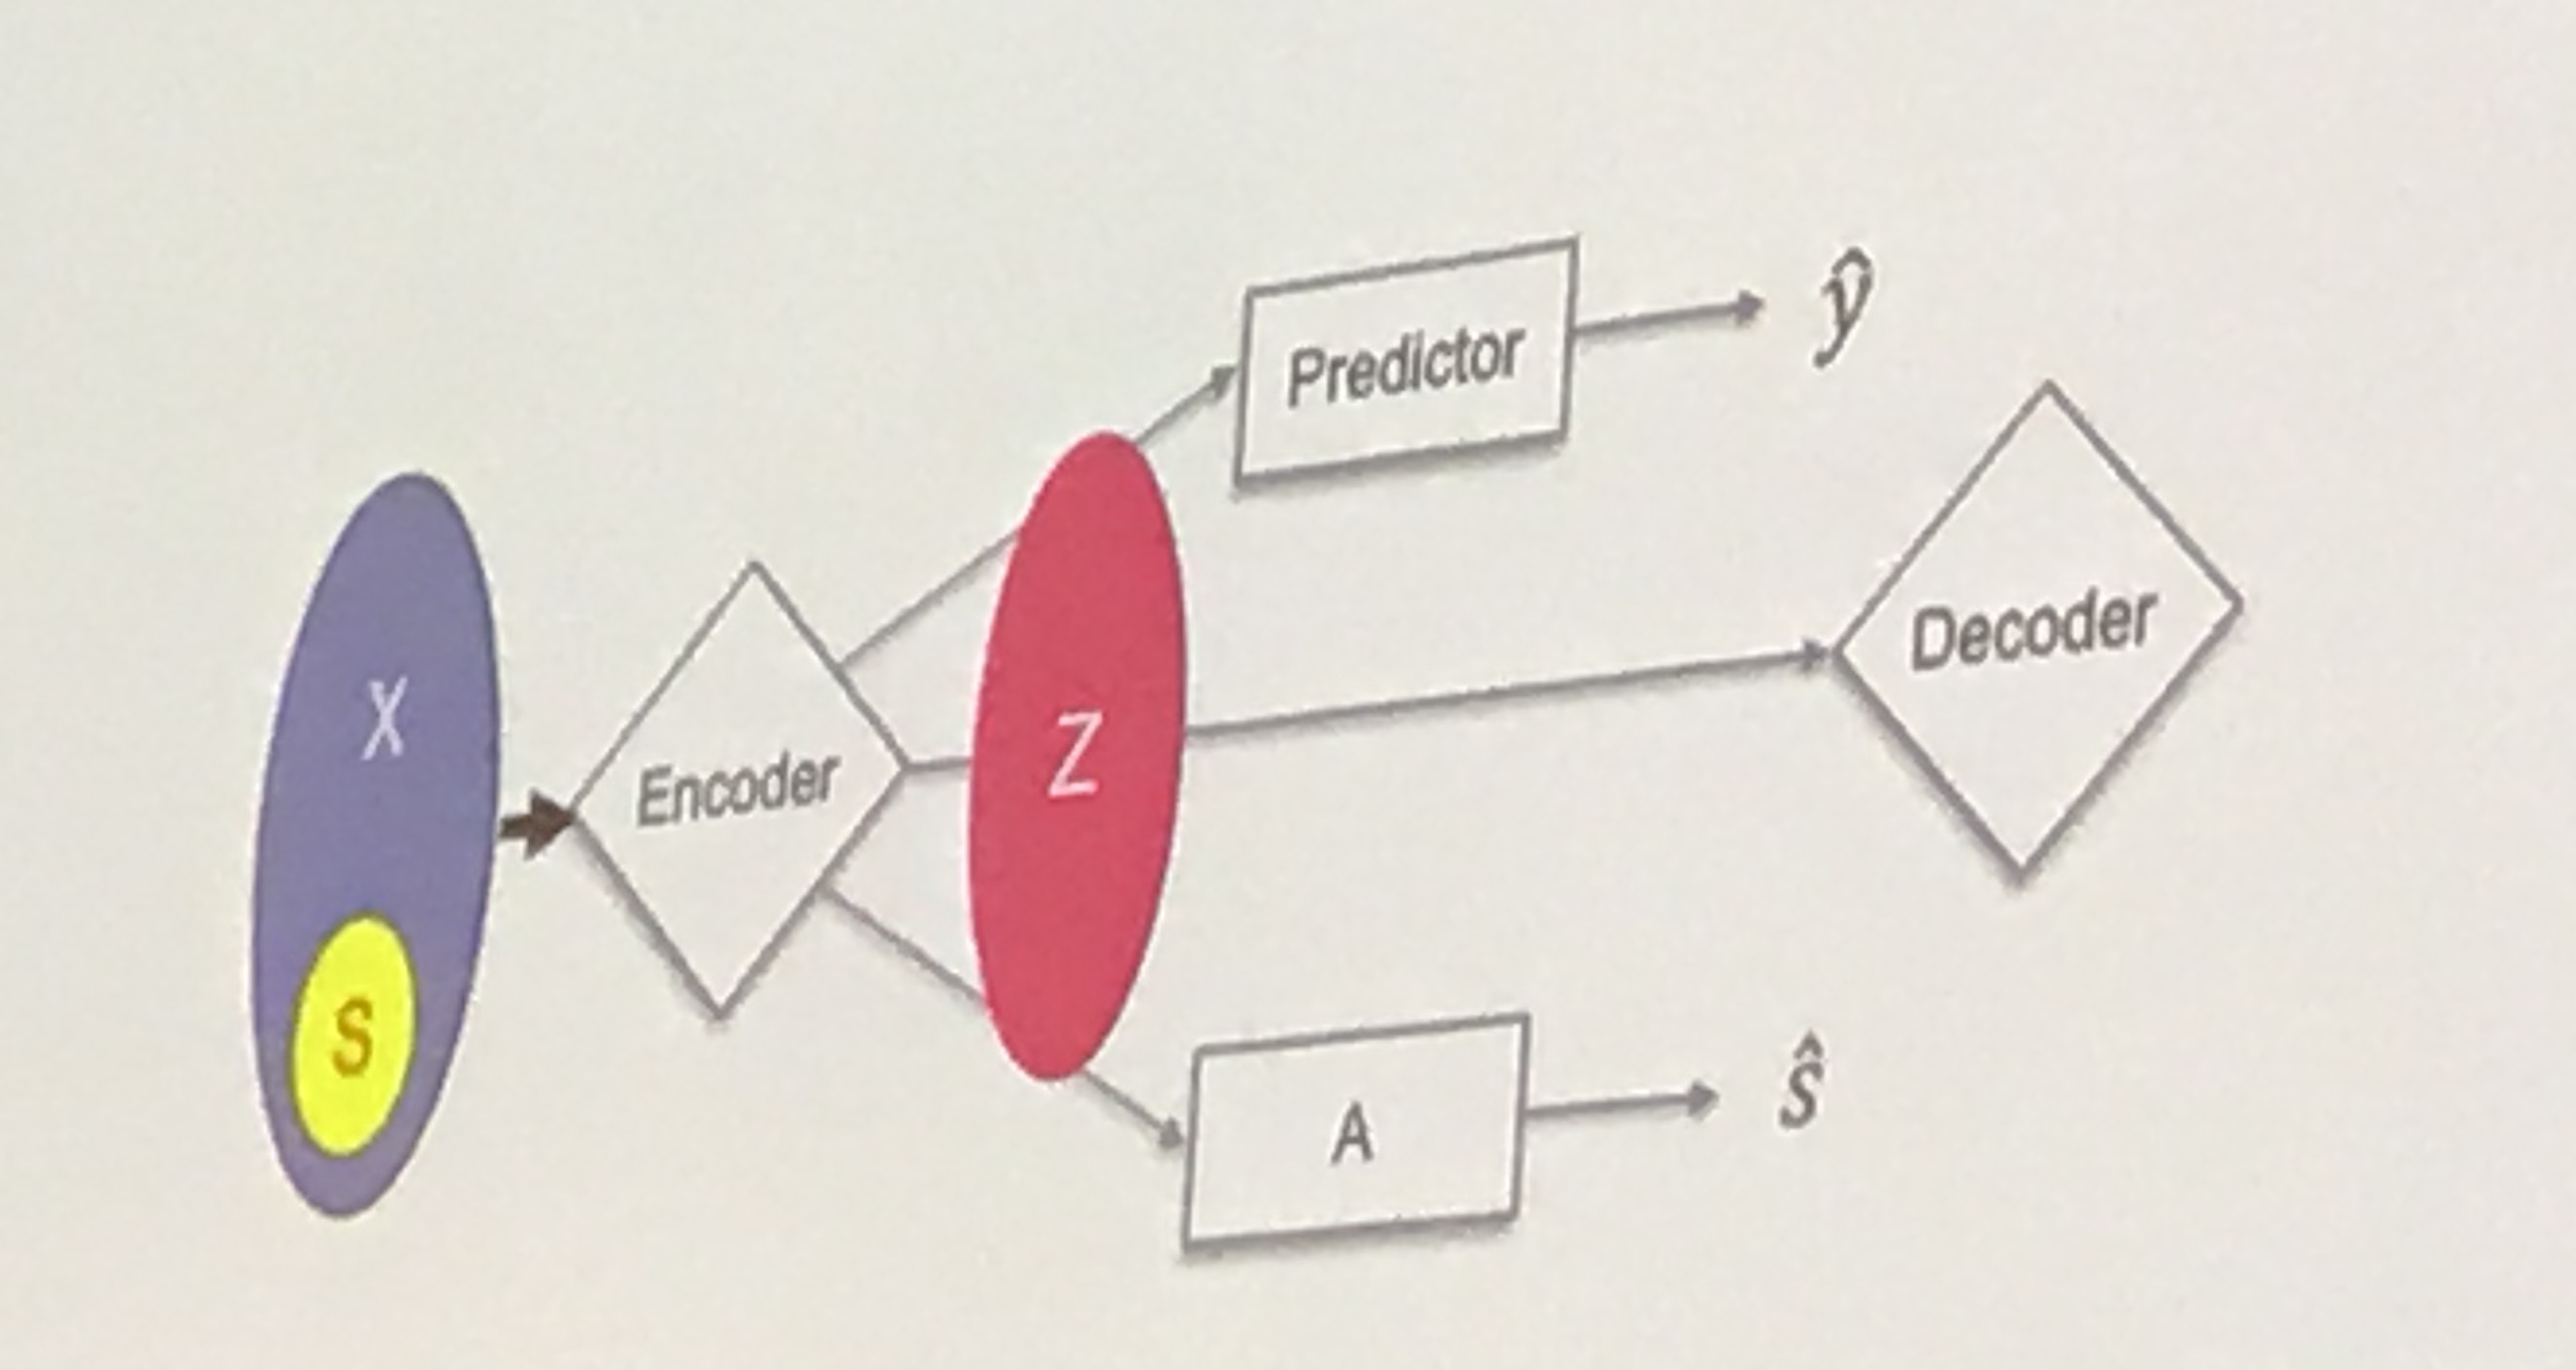
\includegraphics[width=0.4\textwidth]{images/code_rep.png}
    \caption{The cryptographic setup for learning fair representations.}
    \label{fig:my_label}
\end{figure}

{\bf The Harvard-Stanford Problem:} Suppose you're at Stanford, and you build an algorithm for detecting tumors that works really well. Suppose someone else is at Harvard and does the same. \\

$\ra$ Claim: the algorithms wont work across the populations due to differences in the groups and in the lab settings. \\

Goal, then, is to find a way to identify differences/similarities across populations so that these methods {\it can} be transferred across populations.

Approach:
\begin{itemize}
    \item Choose $y \sim Bernoulli(\text{base rate})$
    \item Choose $x \sim N(\mu, \Sigma)$
    \item Retain $x$ if $Bernoulli(\sigma(f_1,s_1)) = f_26i(x_2) = y$.
\end{itemize}


Summary:
\begin{itemize}
    \item A fair algorithm is only one piece of an unfair world
    \item Multiple kinds of fairness: group, individual, Multi-X.
    \item Breakthrough in metric learning for individual fairness
    \item Individual probabilities are hard to understand, but we can  learn from fairness methods to improve their use.
    \item Censered representations and out-of-distribution generalization.
\end{itemize}

\spacerule


Now off to the Structure and Priors in Reinforcement Learning workshop!


\subsection{SPiRL Workshop}

First, Pieter Abbeel on Model-based RL!

\subsubsection{Pieter Abbeel on Model-Based RL from Meta RL}

Few-shot RL/Learning to RL: we have a {\it family} of environments, $M_1, M_2, \ldots, M_n$. Hope is that when we learn from these $n$ environments, we can learn faster on environment $M_{n+1}$. \\

Fast Learning:
\begin{equation}
    \max_\theta \bE_M \bE_{\tau_M} \left[\nsum R_\tau_M^i \mid \text{RLAgent}_\theta \right].
\end{equation}

Objective is roughly the above, where we ground \text{RLAgent}$_\theta$ as an RNN (or some othe generic computational architecture). \\

Other ways to solve this objective like Model-Agnostic Meta Learning (MAML)~\cite{finn2017model}. \\

{\bf Point:} Family of methods that let you train quickly in new environments (new $R$, $T$), given interactions with prior environments. \\

Motivation for Simulation:
\begin{itemize}
    \item Less expensive (can't break robot)
    \item Faster/more scalable
    \item Easier to get lots of labels
\end{itemize}

Q: How can we leverage {\it crude} simulation through domain randomization?  \\

$\ra$ Think about minecraft -- there's some visual structure that is useful for learning about the world, but it's not perfect. How can we train in minecraft (or similar domains) and transfer to the world? \\

A: Randomize aspects of simulations in order to make training of vision system easier. Can then transfer these trained perceptual classifiers to the world, and it works! (same goes for grasping) \\

A: Same goes for grasping -- can train to grasp in simulation, then grasp real objects (with around 80\% success rate). \\

{\bf Result:} Train a hand controller (for manipulating a block in hand) in simulation, can actually deploy it on a real robot. \\

\ddef{Model-Free RL}{Interact with the world and collect data $D$. Then, use this data to inform $\pi$ or $Q$, and use those to act.}

\ddef{Model-Based RL}{Interact with the world and collect data $D$. Then, use this data to inform a world simulator, $\widehat{M}$, perform simulations in order to act.}

Canonical model-based RL;
\begin{enumerate}
    \item For iter $ = 1, 2, \ldots$
    \item \hspace{6mm} Collect data under current policy
    \item \hspace{6mm} Improve learned simulator from all past data
    \item \hspace{6mm} Use simulator to act and collect new data.
\end{enumerate}

{\bf Problem:} learned models are imperfect!  \\

{\bf Fix:} Learn a better simulator. But, this is insufficient. Extremely hard to learn the {\it right} simulation. \\

$\ra$ New overfitting challenge in model-based RL. Policy optimization tends to exploit regularities in simulator, leading to catastrophic failures. \\

{\bf Key Idea:} Don't need to learn an accurate model, just need to learn a set of models representative of the real world (and do few-shot RL):
\begin{enumerate}
    \item For iter $ = 1, 2, \ldots$
    \item \hspace{6mm} Collect data under current adaptive policies, $\pi_1, \ldots, \pi_k$
    \item \hspace{6mm} learn ENSEMBLE of $k$ simulators from past data.
    \item \hspace{6mm} meta-policy optimization over ensemble
    \item \hspace{12mm} new meta-policy $\pi_\theta$
    \item \hspace{12mm} new adaptive policies $\pi_1, \ldots, \pi_k$.
\end{enumerate}

Experiments: 
\begin{enumerate}
    \item {\it MuJoCo:} With about 45 minutes of real interaction with the mujoco environment, state-of-the-art model-free methods can't learn, while the meta-learning approach can.
    \item {\it Robots:} Similarly, can train meta model-based RL in a sample efficient way to learn to perform robotic grasping tasks.
    
    $\ra$ Between 10-100$\times$ more efficient than model-free methods {\it to get to the same asymptotic performance.}
\end{enumerate}

\begin{figure}[h!]
    \centering
    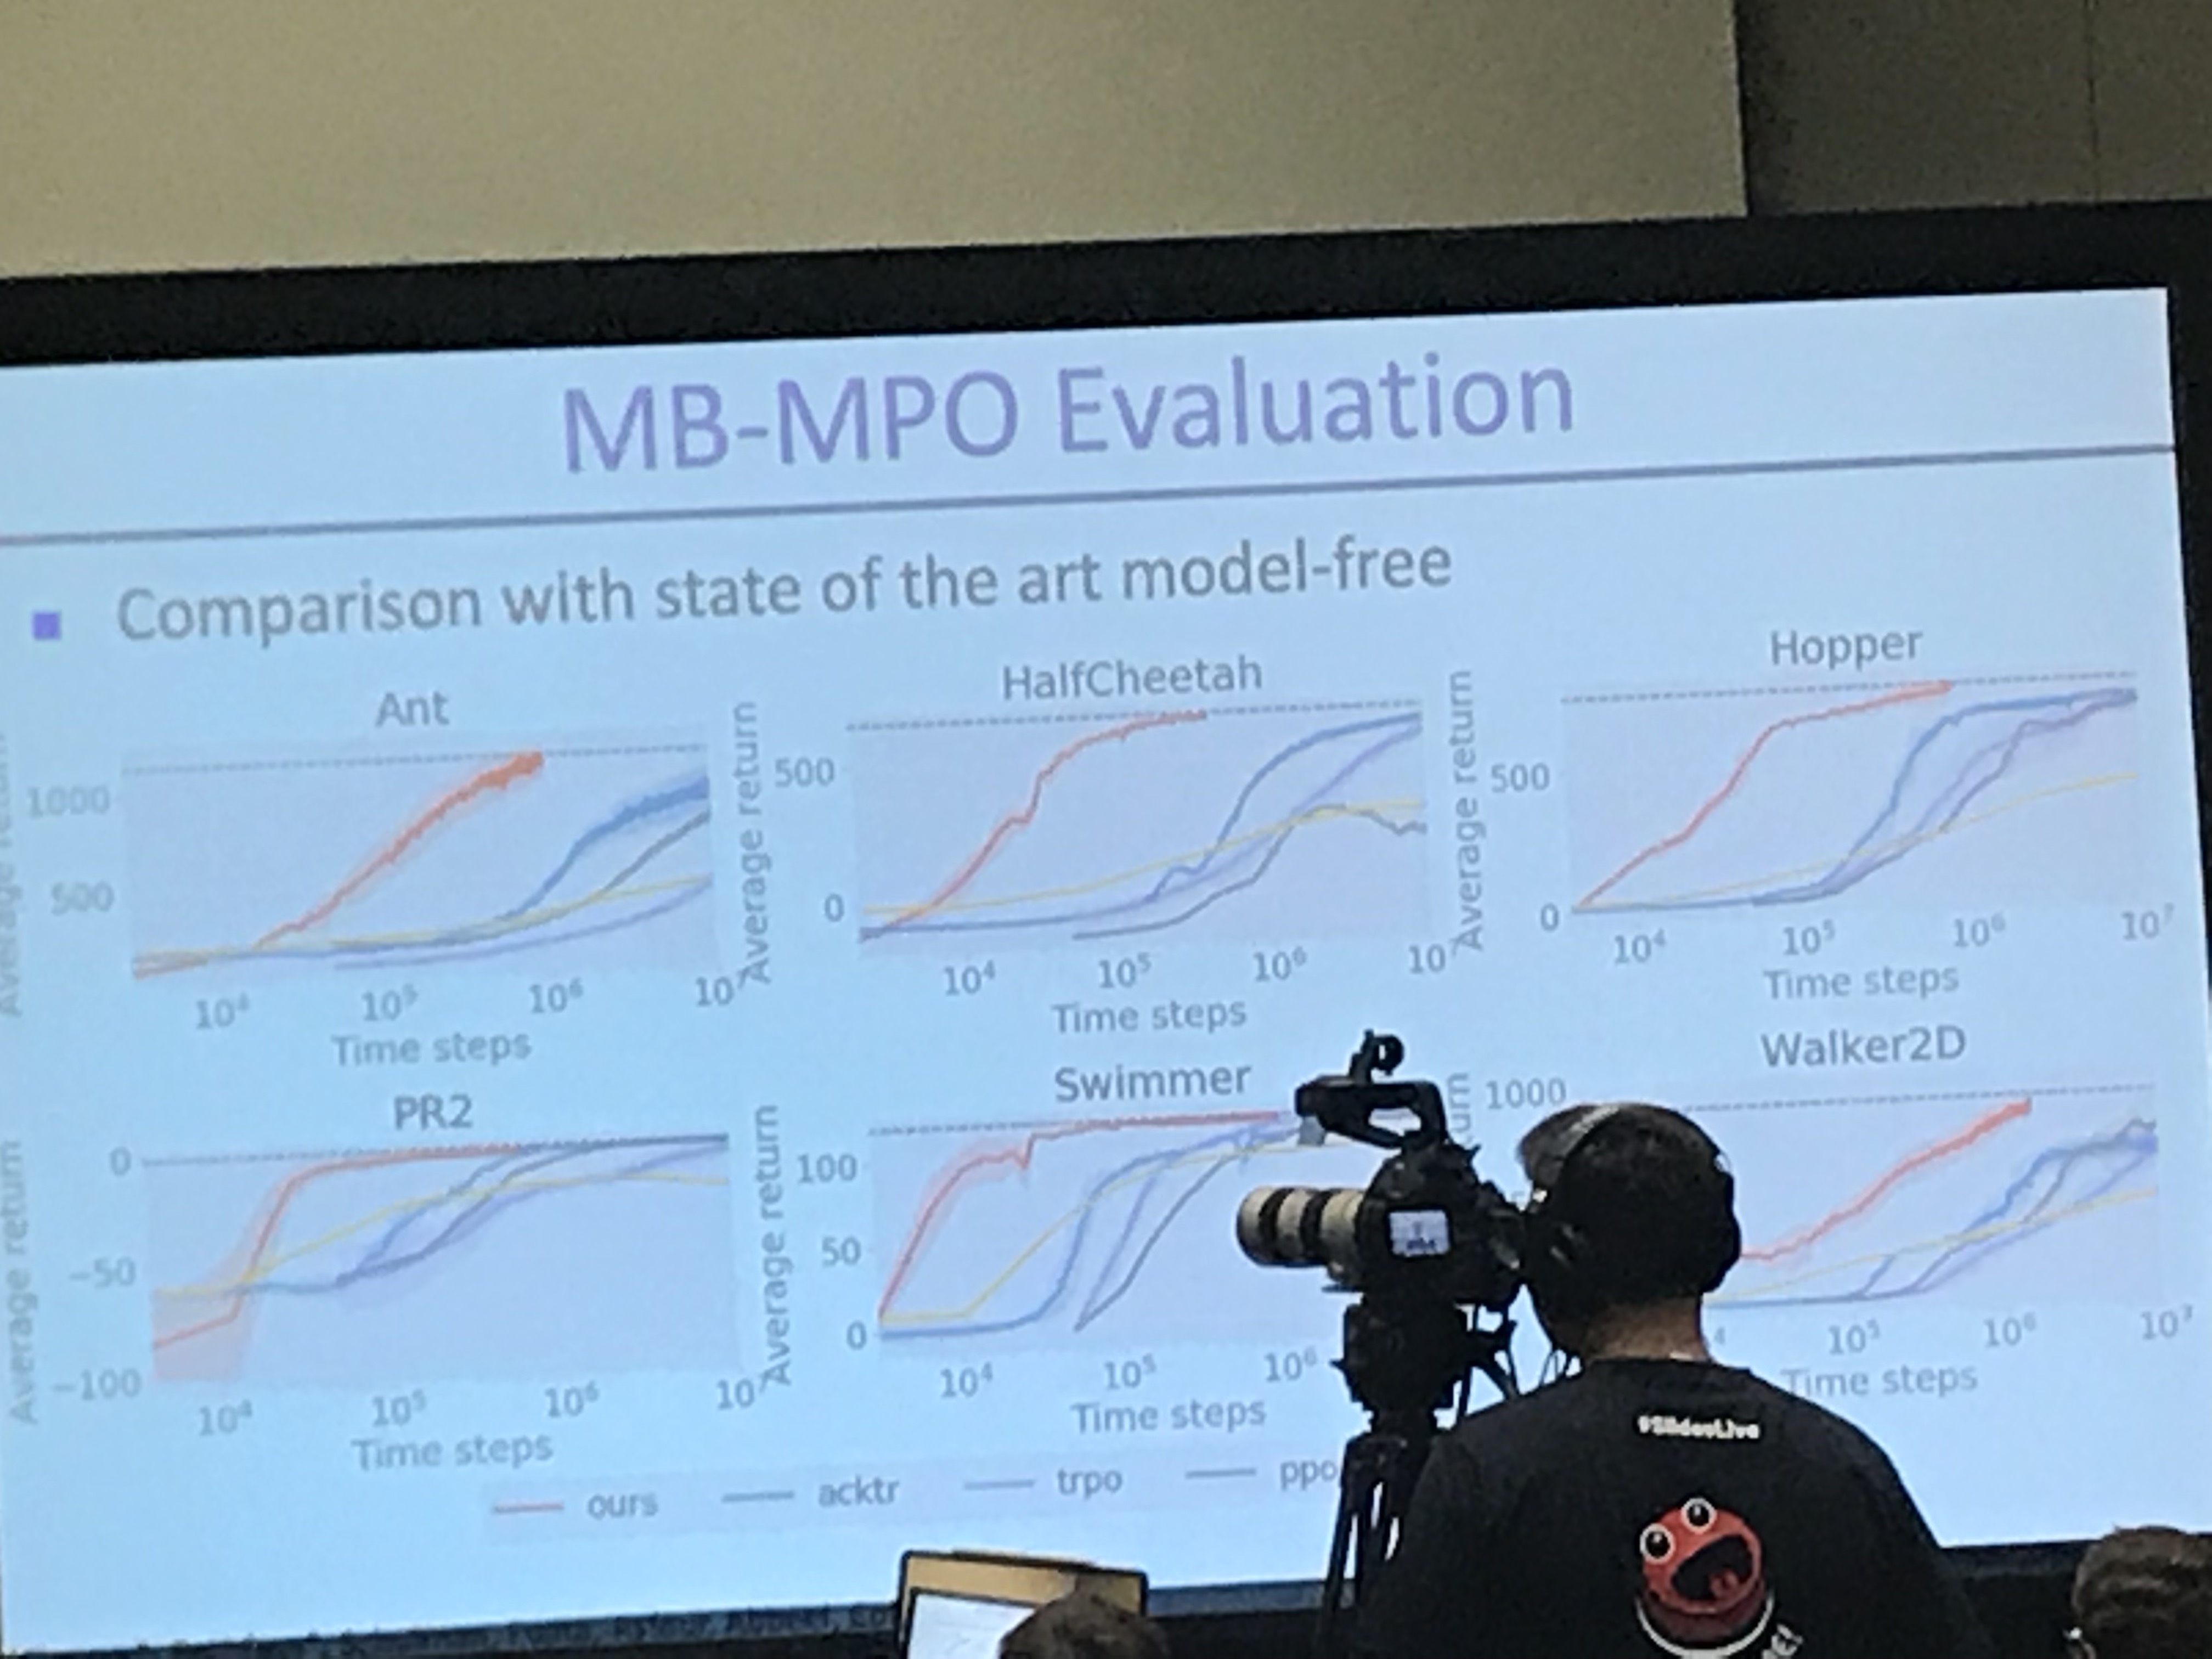
\includegraphics[width=0.4\textwidth]{images/mbrl_results.JPG}
    \caption{Results from meta model-based RL (and a camera + person).}
    \label{fig:meta_mbrl}
\end{figure}


{\it Challenge Question:} Hierarchical RL promises to solve long horizon planning problems. \\

Q1: Are model-free and model-based HRL fundamentally different approaches or are they the same? \\

Q2: Do you think there's a way to combine these two? \\

Pieter A: Yeah absolutely! The methods we presented do some work to combine these methods together. For HRL it might be a bit different, though. In some sense, at the high level, humans don't do RL. We don't have enough ``high level" trials to explore things like ``go to conference/do a PhD". So, the higher level is probably model-based and more planning based rather than RL. Another thing that comes to mind is that HRL approaches seem to only have two levels. One interesting direction is to generalize with more depth/levels rather than two levels. Still not obvious where the separation between model-based/model-free methods takes place. \\

Q: Pros and Cons of looking for an end-to-end approach as opposed to a more modular approach (with more intermittent structure like state estimation). \\

Pieter A: There's no final answer here -- state estimation sometimes involves human provided information, might lose the wrong data for doing control (what is state for a self driving car, for instance?). But, some priors in this way can probably help!


\subsubsection{Contributed Talk: Kate Rakelly on Off Policy RL via Context Variables}

{\bf Goal:} Design agents that are skilled a variety of different tasks. \\

$\ra$ But, training agents in new tasks is statistically/computational infeasible, so really we'd like to exploit shared structure across tasks. \\

{\bf Approach (High-Level):} Meta-RL to learn shared structure across related tasks. \\

Problems: Rapid adaptaion requires efficient exploration strategies, while meta-training requires data from each task, exarcerbates sample inefficiency. \\

{\bf Approach (Detailed View):} Meta-RL via an {\it off-policy} approach. But, raises a problem with exploration since we no longer control the experience distribution. \\

``Context": task-specific information learned from a task ($z$). Meta-training then has two pieces:
\begin{enumerate}
    \item Learn to summarize the context into $z$.
    \item Learn to take actions given $s,z$.
\end{enumerate}

{\bf Algorithm:} \textsc{Pearl}. Given a new task, main idea is to maintain a probability distribution over which task we're in. This lets us exploit knowledge of uncertainty to adapt efficiently to the new task. \\

{\bf Experiments;} four different mujoco domains (half cheetah, humanoid, ant, walker). Rewards and dynamics change across tasks (locomotion direction, velocity, joint parameters). 

Summary:
\begin{itemize}
    \item \textsc{Pearl} is the first off-policy Meta-RL algorithm
    \item 20-100$\timex$ improved sample efficiency on the domains tested
    \item Posterior sampling for efficient exploration during adaption.
\end{itemize}

Code: \url{github.com/katerakelly/oyster} \\

Posters now for a bit.





\subsubsection{Matt Bottvinick on Meta-RL: An Appreciation}

{\bf Point:} We need some structure to scale RL. What I have in mind is something like relational RL, objects, graph nets, and so on. \\

Guiding Question: What do the algorithms that meta-RL gives rise to, do? What can't they do? \\

Recent survey summarizing some of the ideas~\citet{botvinick2019reinforcement}. \\

$\ra$ The field seems to have moved on from meta-RL, but I can't! Let's really understand these algorithms. \\

Tendency: let's build a faster race car. This talk: let's understand fast race cars, or why these things we've made recently are fast! \\

Observations in trying to understand Meta-RL:
\begin{itemize}
    \item Consider two-armed bandits: An animal chooses between two arms, payoff determined according to some payoff schedule. Critically, sources of reward get restocked every so often. 
    
    $\ra$ Animals match their frequency in choices with the frequency with which they get rewards (probability matching).
    
    $\ra$ Ordinary LSTM figures that out, too! Also figures out the gittins optimal thing in the regular $\beta-Bernoulli$ bandit.
    
    \item Consider this new bandit task: probabilities of payoff keep changing, but volatility changes, too (long intervals where payoffs flip around, etc.).
    
    $\ra$ Smart thing is to change your learning rate. People do in fact do this (if we fit a model predicting learning rates to peoples' decisions).
    
    $\ra$ Meta-learned LSTM can do the same thing!
    
    \item Monkey sees two colored face down cups, one of which hides a raisin. Learn to pickup the cup hiding the raisin in general.
    
    $\ra$ Then the monkey has to transfer to a new task with new objects. Turns out monkey learns to transfer as well; when no info can be used, monkey explores uniformly, when info can be exploited, monkey learns very quickly.
    
    $\ra$ LSTM can do this, too!
\end{itemize}

Clear illustration of a meta model-free algorithm giving rise to a model-based RL, based on model-based tests designed for people/animals from~\citet{daw2014algorithmic}. \\

\begin{figure}[h!]
    \centering
    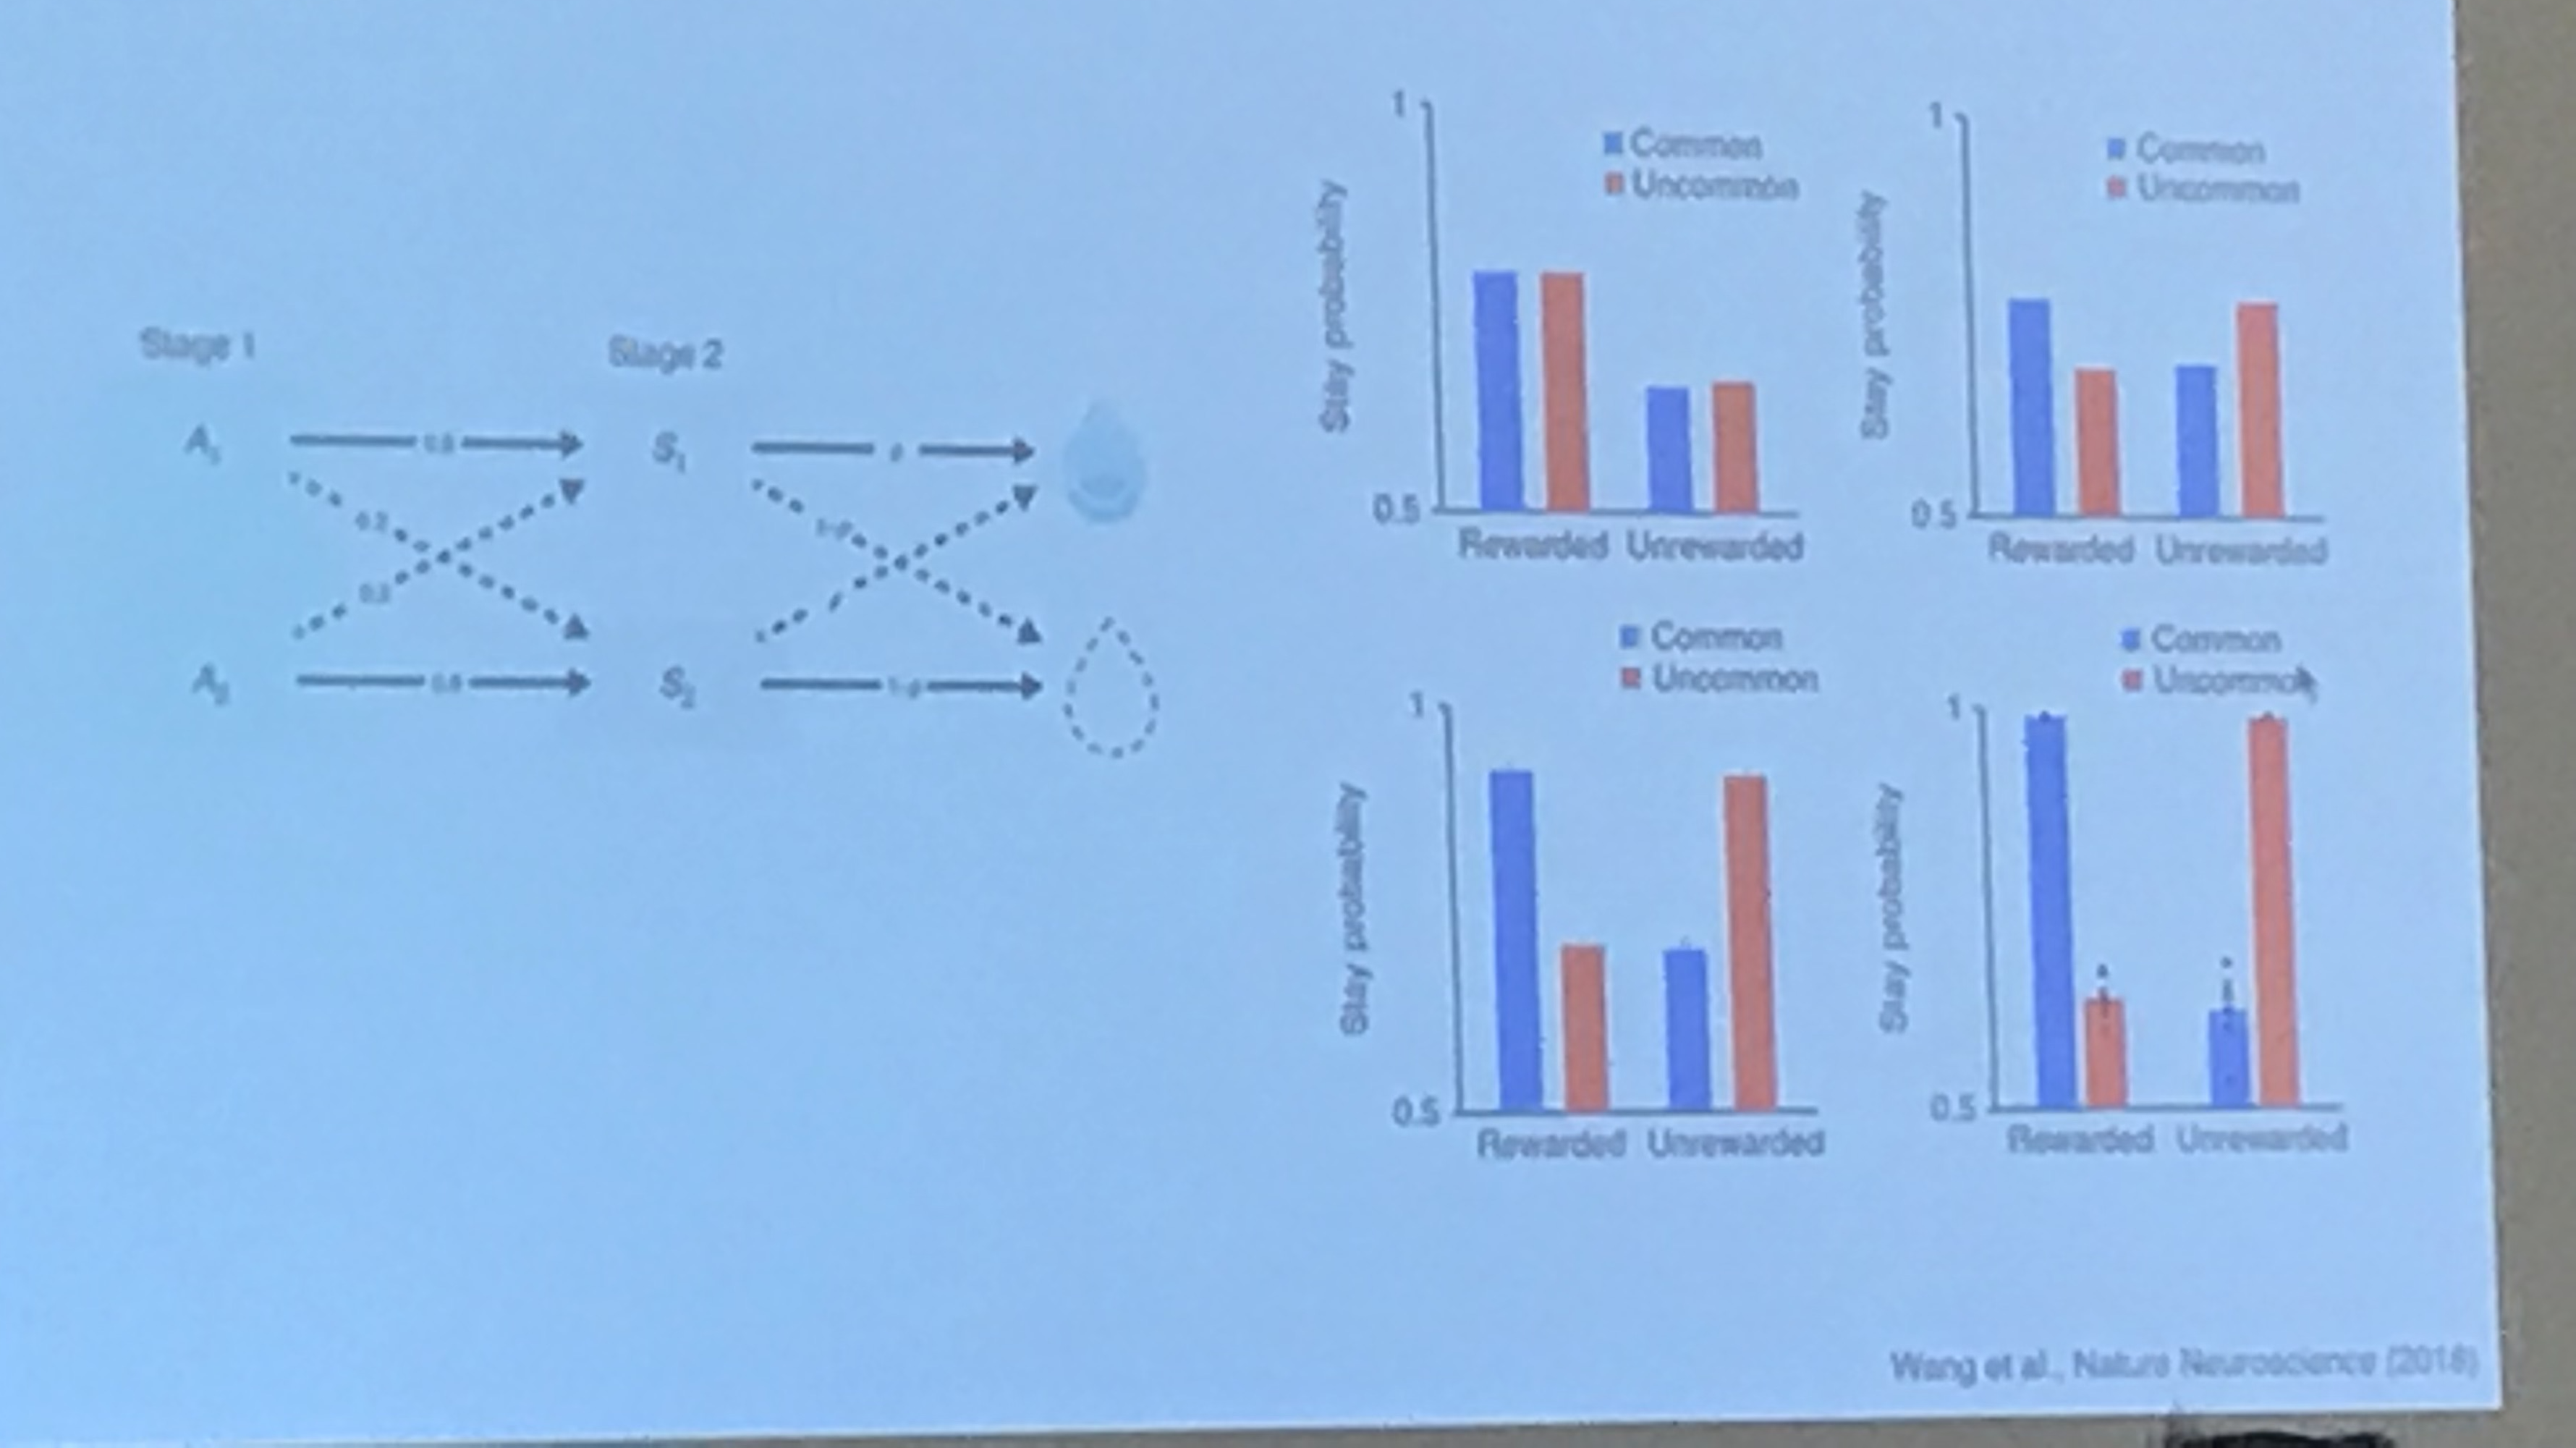
\includegraphics[width=0.4\textwidth]{images/mb_task.png}
    \caption{A task for determining whether a decision making is using model-based techniques or not (left) and results from different approaches on the task (right).}
    \label{fig:mb_task}
\end{figure}

{\bf Point 1:} Meta-RL can also give rise to algorithms that can solve temporal credit assignment problems, too. \\

{\bf Point 2:} For LSTM to be solving certain kinds of tasks, they also must be retaining some sufficient statistics in their state (that roughly match what the observer would track, too). \\

Lastly: a crazy idea (\dnote{Matt's words, not mine :)}). We have some evidence that with ordinary LSTMs, model-free RL can give rise to model-based RL (in the right situation). \\

$\ra$ Maybe, if we set of the environments in the right way, maybe LSTMs can work out algorithms for doing (amortized?) Bayesian inference. \\

{\bf Take Home Message:} Meta-RL is really exciting, let's keep coming up with faster algorithms but also try to understand what they're doing.

\subsubsection{Katja Hoffman on Challenges \& Directions in Multi-Task RL}

Q: Why do we focus on structure and priors in RL? \\

Katja A: Three things!
\begin{enumerate}
    \item Improve sample efficiency
    \item Improve sample efficiency
    \item Improve sample efficiency
\end{enumerate}

Q: When you think about structure and priors in RL, what kidns of challenges become solvable? \\

A: Maybe in games, science, transporation, medicine? \\

$\ra$ For these (and probably other) domains, structure is crucial. \\

%Q: Who will have access to these solutions? \\

Kinds of Structure:
\begin{itemize}
    \item Assume multiple related tasks and useful relationship between tasks can be learned from data
    \item Q: What types of models allow learning and use of related task structure>?
    \item Q: What trade-offs can we achieve between prior assumptions, flexibility, and sample efficiency?
\end{itemize}

First Approach: Meta-RL with Latent Variable Gaussian Processes~\cite{saemundsson2018meta}. IDea:
\begin{itemize}
    \item Problem: assume $p$ task with related dynamics:
    \begin{equation}
        y_t^p - f(x_i^p, h_p) + \eps,
    \end{equation}
    \item Observe data from training tasks
    \item Goal: accurately predict held out test dynamics with minimal additional data

    \item Approach: Model-Based RL via latent variable Gaussian processes. Place a GP prior on global function.
    
    \item Experiments: 1) toy taks, mult-task prediction. Approach is able to disentangle unseen tasks; 2) multi-task cart pole. System can cary in mass and pendulum length, many held out settings of these parameters.
\end{itemize}

Second Approach: (CAVIA) Fast Context Adaptation via Meta-Learning~\cite{zintgraf2018caml}.
\begin{itemize}
    \item Problem: distribution over training and test task $p_{train}$, $p_{test}$.
    \item During meta-training, sample tasks from $p_{train}$, get train/test data for that task
    \item Learn how to adapt quickly on the task by splitting up network into: 1) task specific context parameters $\phi$, and 2) shared parameters $\theta$.
    \item Experiments: 1) supervised learning task; 2) multi-task half cheetah.
    
    $\ra$ CAVIA learns an itnerestable task embedding, captured in context parameters
    $\ra$ Adapts to test tasks with updates to only context parameters -- sheds new light on meta-learning benchmarks.
    $\ra$ Very flexible
\end{itemize}

Follow up: Variational Task Embeddings for Fast Adaptaion in Deep RL. Learns to trade of exploration and exploitation online, while interacting with the environment. VATE can deduce information about the task before seeing any reward. \\


{\bf Point:} As we push forward in RL to harder domains, there might be certain generic structure that tends to work well across many domains. Can we find this unifying structure? \\

$\ra$ One thing that might be needed is a dataset that might rive rise to such structure. To this end: \\

$\ra$ MineRL: competition (\url{minerl.io/competition}) on sample efficient RL using human priors (upcoming at NeurIPS this year), built on top of MALMO~\cite{johnson2016malmo}. \\

Minecraft is massively complex, so offers a great platform for exploring the use of priors in RL. See Figure~\ref{fig:mc_tree} for a sense of the size of the tech tree.

\begin{figure}[h!]
    \centering
    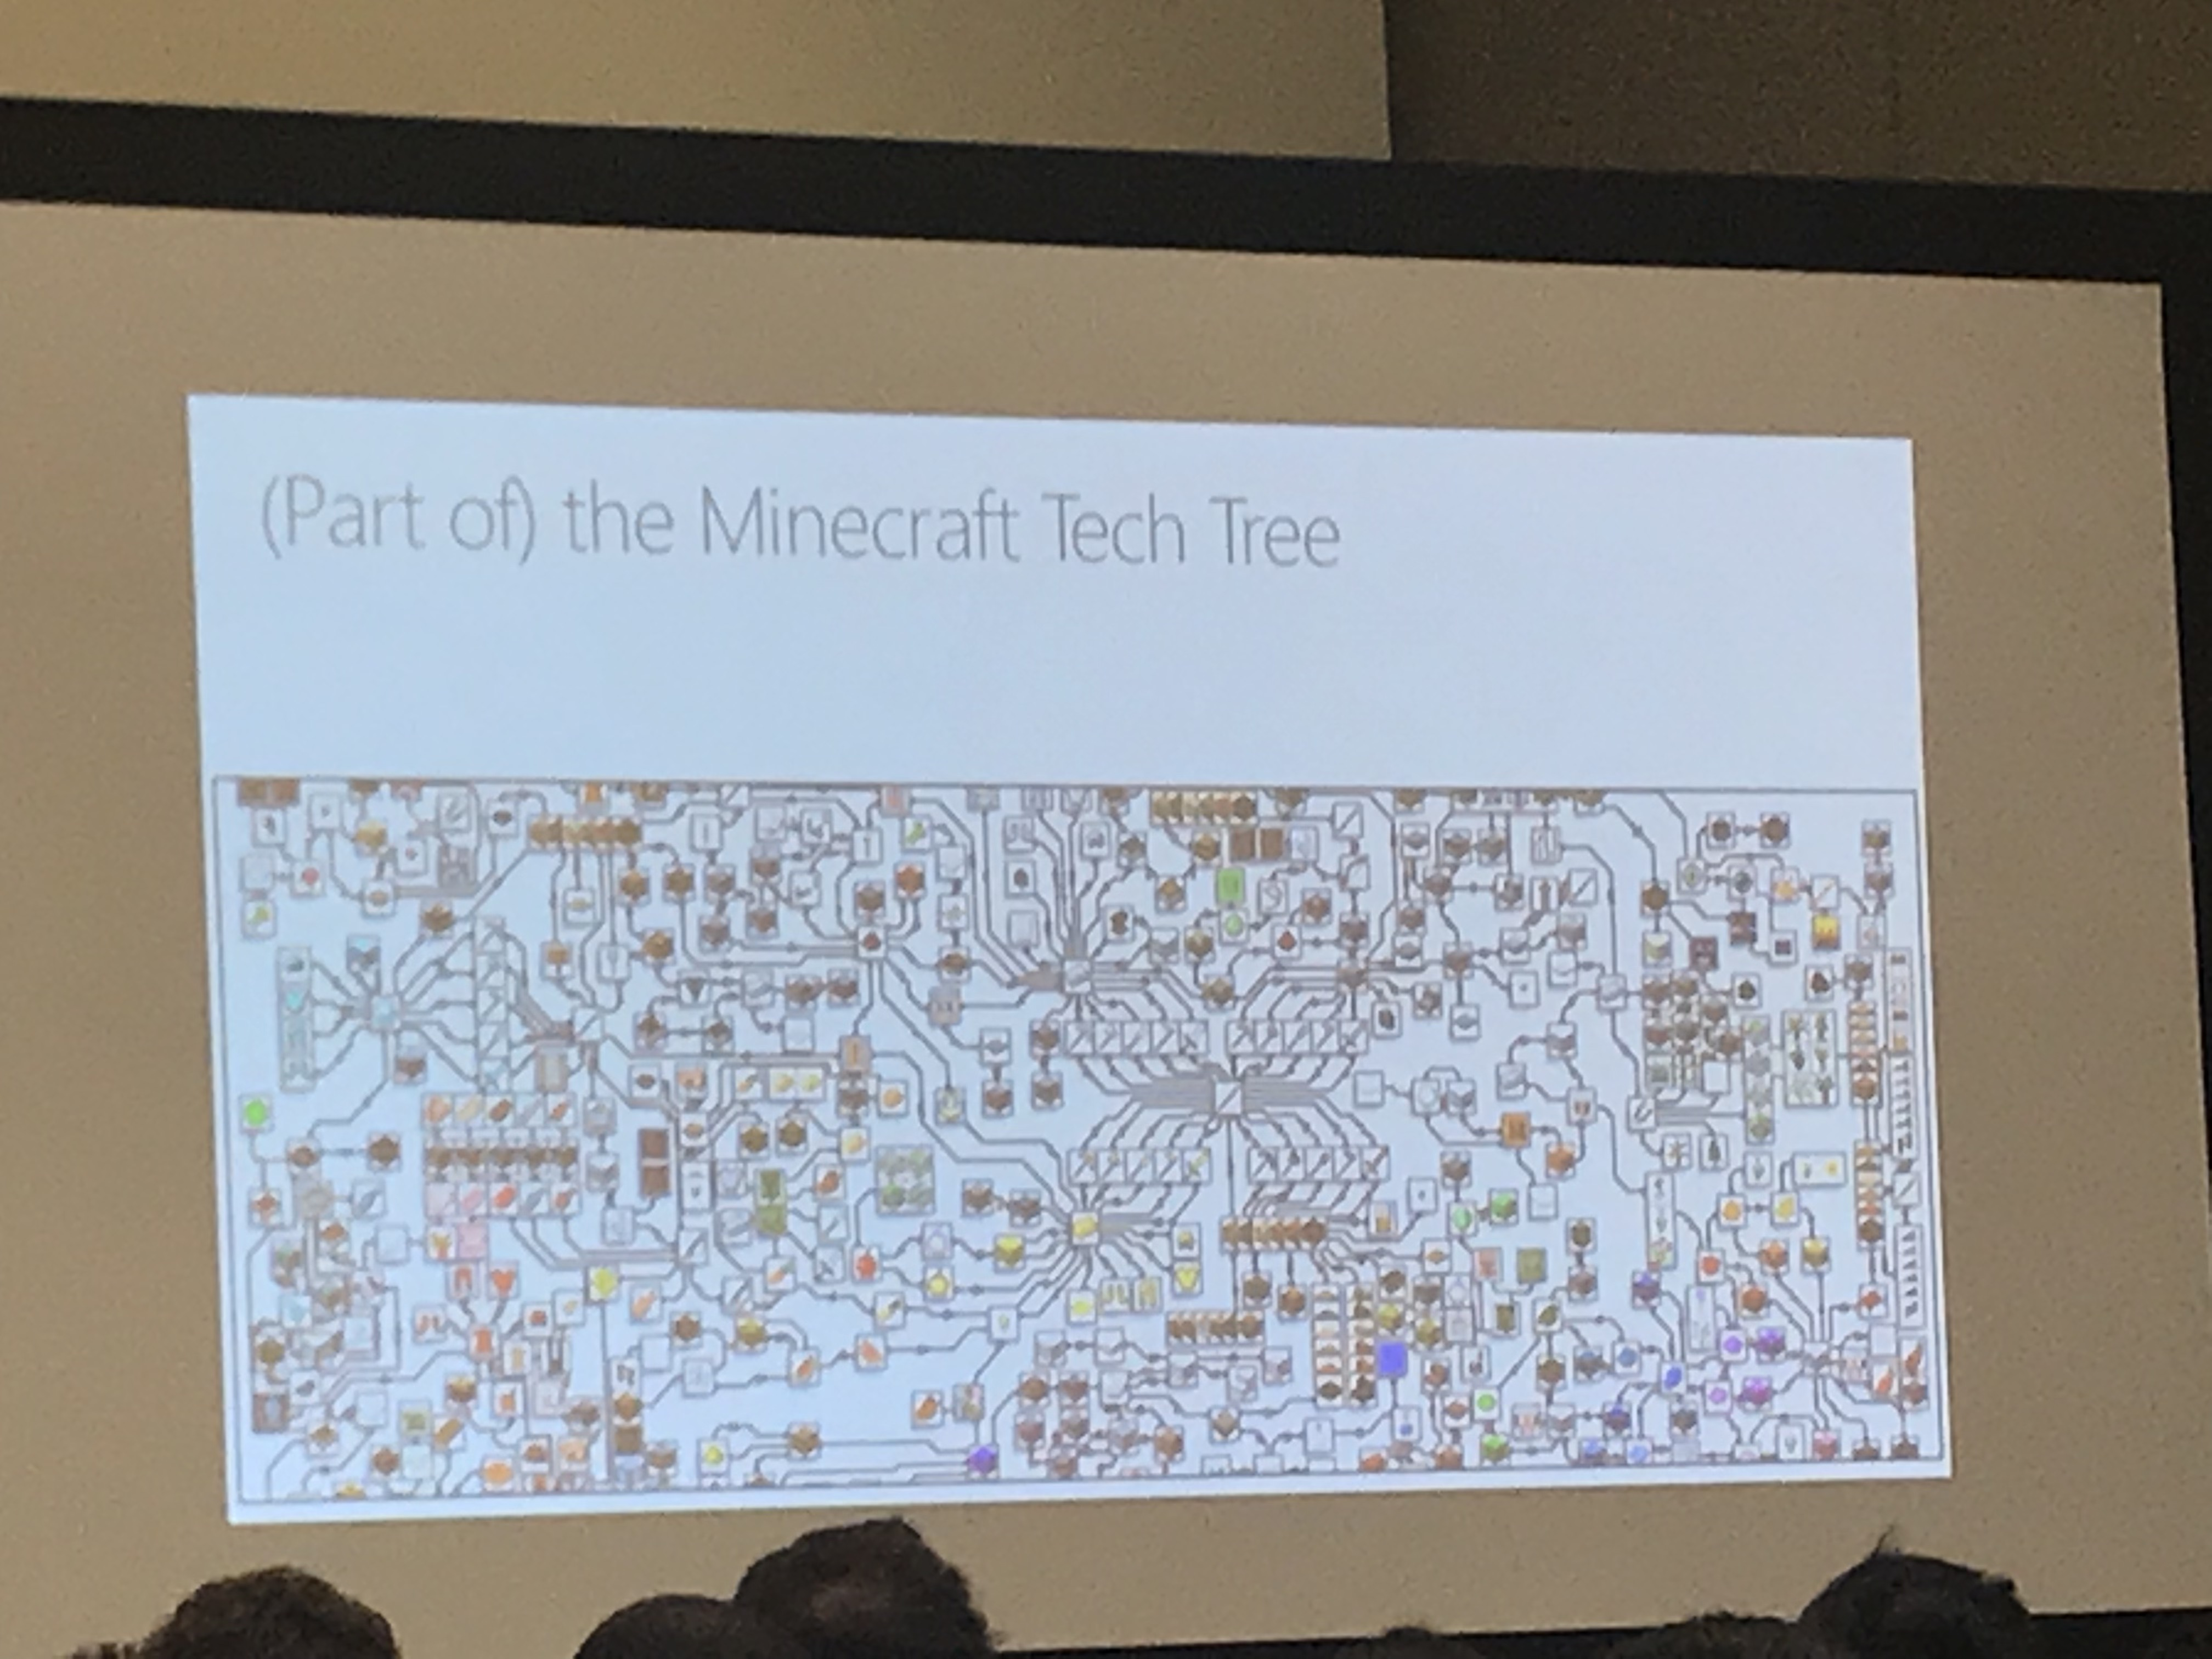
\includegraphics[width=0.4\textwidth]{images/mc_tree.JPG}
    \caption{Part of the tech tree in Minecraft}
    \label{fig:mc_tree}
\end{figure}

\subsubsection{Tejas Kulkarni on Object-Centric Representations RL}

{\bf Point:} The hard problems of RL:
\begin{enumerate}
    \item State estimation
    
    RL does not prescribe a detailed recipe to represent state. Hand specify or learn a state representation.
    
    \item Exploration
    
    And: how you explore depends on how you explore the world.
\end{enumerate}

This work: let's use self-supervised deep learning to learn object structure. \\

Example: an individual blind from birth can still draw rough object structure, including {\it perspective}~\cite{kennedy2006blind} -- see Figure~\ref{fig:drawing}. \\

\begin{figure}[h!]
    \centering
    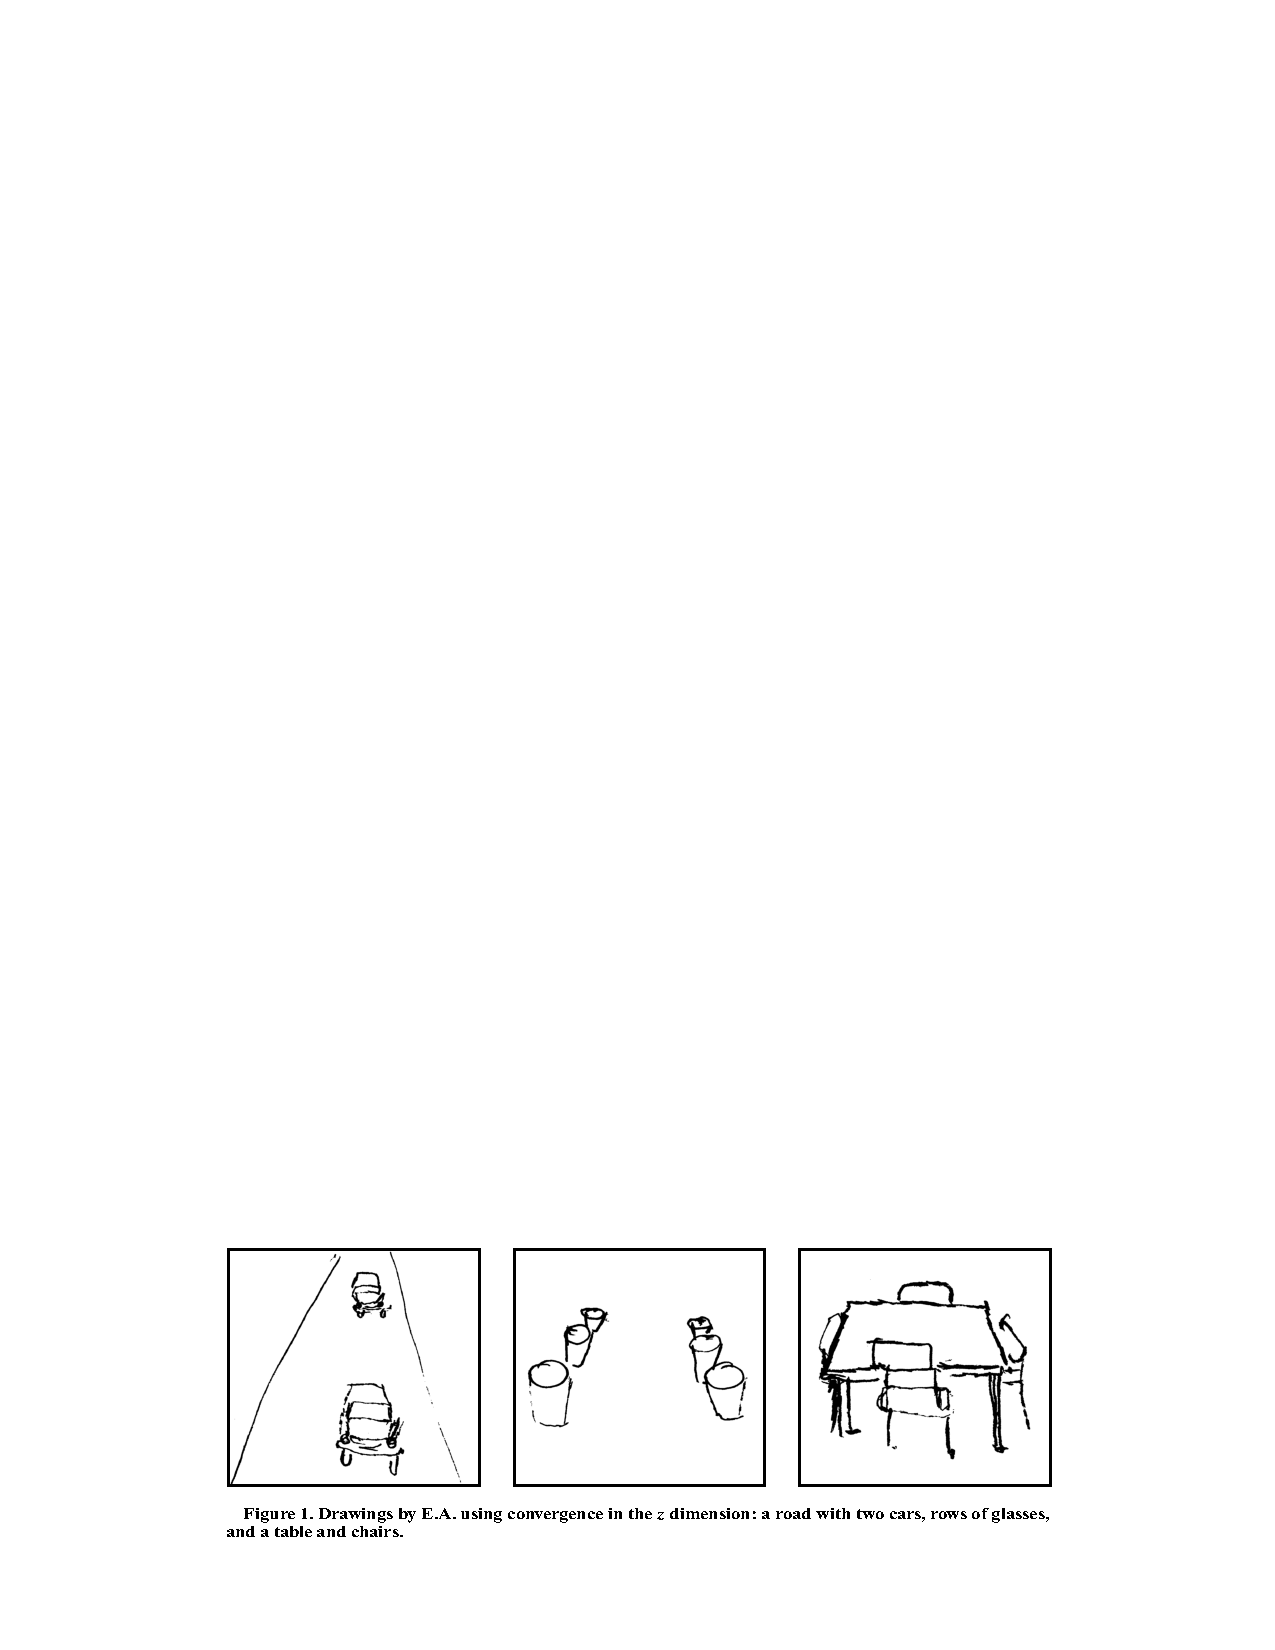
\includegraphics[width=0.5\textwidth]{images/drawing.pdf}
    \caption{Drawings from~\citet{kleinberg2016inherent}}
    \label{fig:drawing}
\end{figure}

Objects in particular are a fundamental and important abstraction.\\

Q: So, can we learn them?\\

Three properties from object-centric representation in physical domains:
\begin{enumerate}
    \item Capture spatio-temporal features at degrees of freedom.
    \item Long-term temporal consistency.
    \item Captures basic geometry of the environment.
\end{enumerate}

A: Yes! The ``Transporter" network (see Figure~\ref{fig:transporter}). %. \\

\begin{figure}[h!]
    \centering
    \subfloat[Transformer Network]{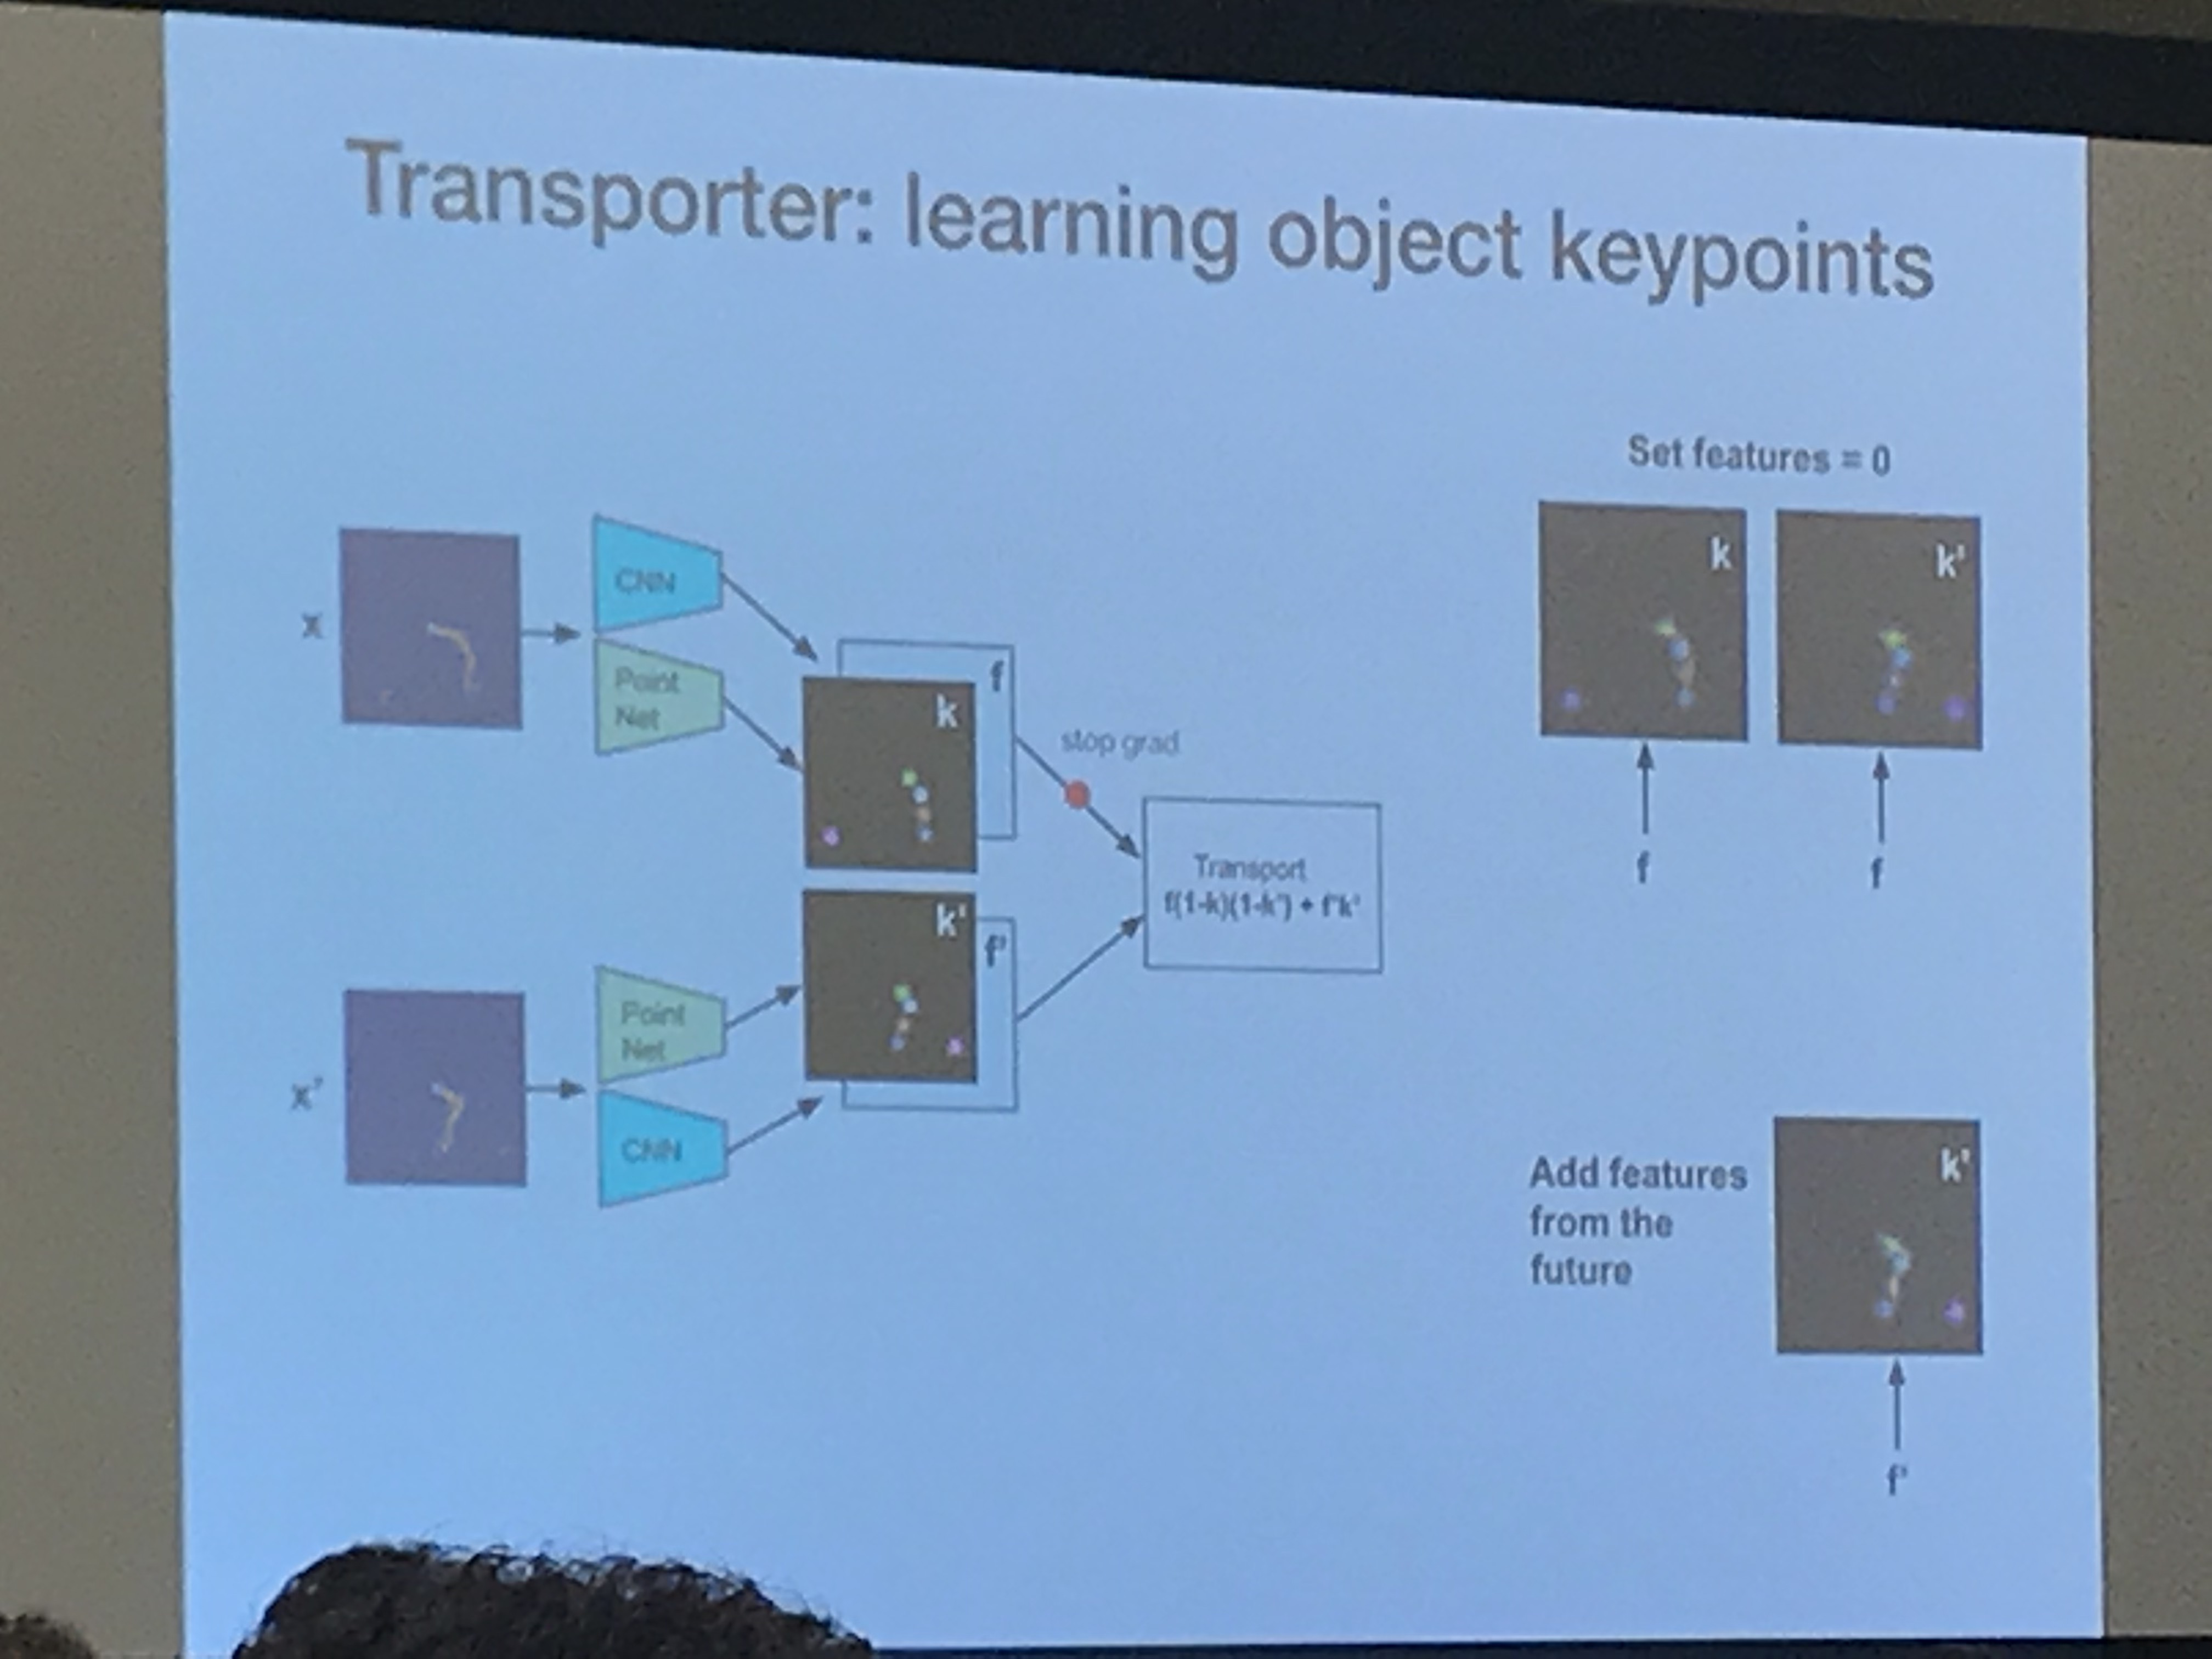
\includegraphics[width=0.4\textwidth]{images/transporter.JPG}} \hspace{5mm}
    \subfloat[Object Classification]{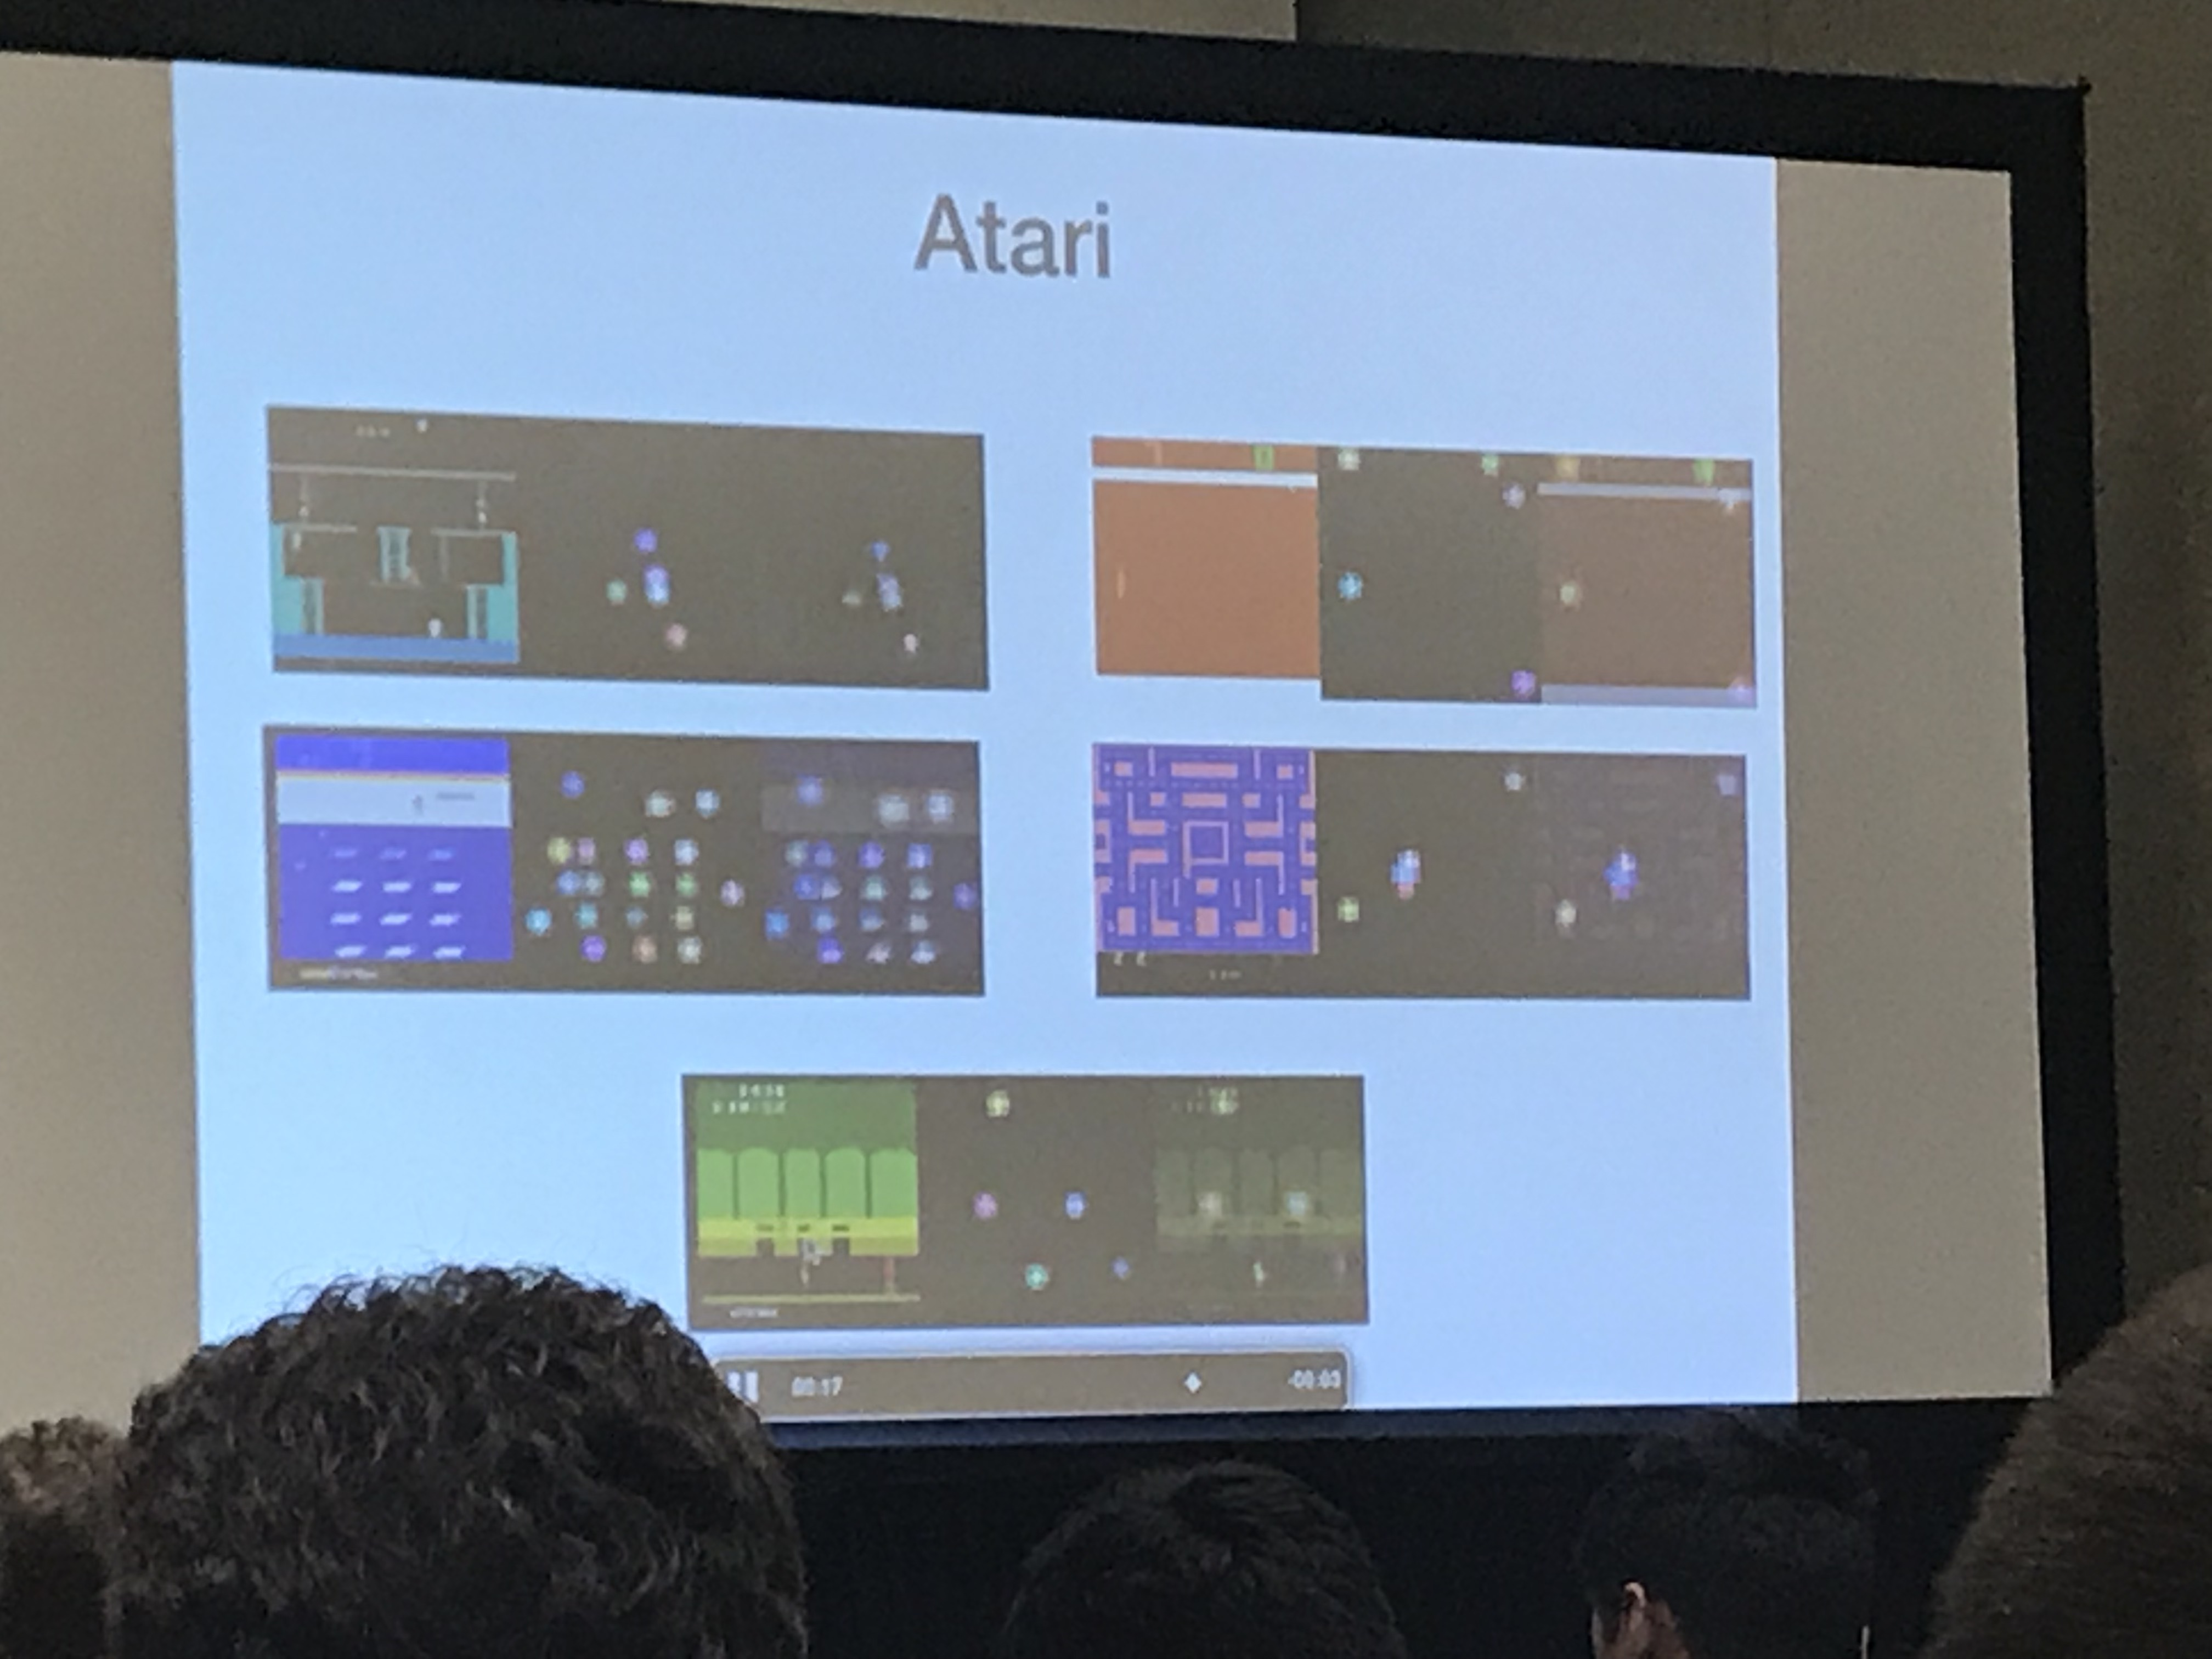
\includegraphics[width=0.4\textwidth]{images/objects.JPG}}
    \caption{Transporter Network (left) maps source to target image via compressed geometric representation, and some candidate objects found (right) in different Atari games.}
    \label{fig:transporter}
\end{figure}

$\ra$ Transporter network does a good job for capturing salient objects in image based problems like Montezuma. Trained on uniform random policy, and the result is a spatial map of where different objects area. \\

But: the above approach only tracks moving objects, not stationary ones. So, we can pair it with instance-based segmentation for finding stationary objects. \\

{\bf Next Stage:} Object-Centric RL and Planning in high dimensional domains, building on the earlier work by~\citet{diuk2008object}. \\

$\ra$ Key Problem 1: Structured exploration in the space of objects and relations. \\

$\ra$ Key Problem 2: Generalization in the form of self generated tasks in the space.

Object-centric HRL architectures~\cite{kulkarni2016hierarchical,dilokthanakul2019feature}. \\

Major frontier: data efficient RL in hard exploration settings like Montezuma. Idea: systematically explore in the space of objects and relations.

{\it Challenge Question:} In supervised learning, progress in representation learning and trasnfer learning for vision has been largely driven by ImageNet. NLP had its ``ImageNet" moment with GPT-2 and BERT. So, will there be a analogous ``ImageNet" moment in RL that allows us to learn general prupose data-driven priors? \\

A: Yeah, absolutely! I think we're almost there. Lots of folks working in this direction, I think we are right around the corner. 


\subsubsection{Tim Lillicrap on Learning Models for Representations and Planning}

Current State and Limitations of Deep RL:
\begin{enumerate}
    \item We can now solve virtually any single task/problem for which:
    \begin{enumerate}
        \item Formally specify and query the reward function
        \item Explore sufficiently and collect lots of data
    \end{enumerate}
    \item What remains challenging:
    \begin{itemize}
        \item Learning when a reward function is difficulty to specify
        \item Data efficiency and mult-task transfer learning
    \end{itemize}
\end{enumerate}

We measure outcomes via: $R(\tau) = \sum_{t=0}^T \gamma^t r_t$, with the objective function:
\begin{equation}
    J(\theta) = \int_\mathbb{T} p_\theta(\tau) R(\tau) d\tau.
\end{equation}

But: In model-free RL we tend to throw away what we know about the task to solve it. \\

Clear structure to introduce: plan with a model. \\

$\ra$ Tricky! Getting this model is really hard. If we can get it, we know it can be really powerful (see AlphaZero~\cite{silver2018general}). \\

{\bf Problem:} Planning with learned models is really hard. (Tim said it became a running joke to started up a model-based RL project at DeepMind in the last few years: no one expected it to work). \\

Idea: Hybrid model-free and model-based approaches. By augmenting previous algorithms with a learned model did in fact help on a goal-finding task. \\

Planning with Learned Models: PETS~\cite{chua2018deep}, Deep Planning Network (Planet)~\cite{hafner2018learning}. \\

Experiments: continuous control from image observations (finger, cheetah, cup, etc). \\

$\ra$ Some versions of this end up working well! Around 1k-2k episodes it can solve image-based mujoco problems. \\

{\bf Conclusions:}
\begin{itemize}
    \item Model-based algorithms hold promise of addressing data efficiency and transfer learning limitations.
    \item Beginning to develop working recipes that allow planning with models in unknown environments.
    \item Necessary and sufficient conditions for planning with learned models are unclear.
    \item Much work remains!
\end{itemize}


{\it Challenge Question:} What are the trade-offs in rolling value estimation and perception into the same architecture? \\

Tim A: I don't know anyone that's systematically studied this kind of thing, but it's definitely important to study it more. Some insights can be gathered from AlphaZero, ELO rating analysis. Lots more to do! 

\subsubsection{Karthik Narasimhan on Task-agnostic Priors for RL}

Current State of RL: success of model-free RL approaches (see: Go, DOTA). \\

$\ra$ All of these feats require huge amounts of time and samples (like 45,000 years of gameplay for DOTA). \\

$\ra$ Little to no transfer of knowledge. \\

Recent Approaches:
\begin{itemize}
    \item Multi-task policy learning
    \item Meta-learning
    \item Bayesian RL
    \item Successor Representations
\end{itemize}

Observation: all approaches tend to learn policies, which are rigid and hard to transfer to other tasks. \\

Solution: model-based RL.\\

$\ra$ Approach: bootstrap model learning with task agnostic priors. The model is 1) more transferrable, 2) expensive to learn but can be made easier with priors. \\

Q: Can there be a universal set of priors for RL? \\

A: Look to how humans learn new tasks. These priors seem to come from 1) a notion of intuitive physics and 2) language. \\

{\bf Project 1:} Can we learn physics in a task agnostic way? Moreover, can this physics prior help sample efficiency of RL? \\

Lots of prior work in this area, but they are task-specific. \\

$\ra$ This work: learn physics prior from task-independent data, decouple the model and policy. \\


Overview of approach:
\begin{itemize}
    \item Pre-train a frame predictor on physics videos
    \item Initialize dynamics models and use it to learn policy that makes use of future state predictions.
    \item Simultaneously fine-tune dynamics model on target environments.
\end{itemize}
Two Key Operations: 1) isolation of dynamics of each entity in the world, 2) accurate modeling of local spaces around each entity. \\

Experiments: PhysWorld and Atari -- in both cases, use videos containing demonstrations of the physics of the environment to do some pre-training of the dynamics model (in Atari, pre-training is still done in PhysWorld). Results show the approach works very well, both at 10-step prediction and at helping sample efficiency in RL. \\


{\bf Project 2:} Can we use language as a bridge to connect information we have about one domain to another, new domain? \\

Overview of approach:
\begin{itemize}
    \item Treat tanguage as task-invariant and accessible medium.
    \item Goal: transfer a model of the environment using text descriptions.
    
    Example: ``Scorpoins can chase you". Might be able to learn a model that places high probability on the scorpoin moving closer to tthe agent location.
    
    \item Main technique: transfer knowledge acquired from language to inform a prior on the dynamics model in a new environment.
\end{itemize}


Conclusions:
\begin{enumerate}
    \item Model-based RL is sample efficient but learning a model is expensive
    \item Task agnostic priors over models provide a solution for both sample efficiency and generalization
    \item Two common priors applicable to a variety of tasks: classical mechanics and language.
\end{enumerate}


{\it Challenge Question:} Lots of success in Deep RL. New push into hybrid approaches like cross-domain reasoning, using knowledge from different tasks to aid learning, and so on. What are the greatest obstacles on the path to mid-level intelligence? \\

Karthik A: I would emphasize the need for distributional robustness and transfer -- need to look at agents that can transfer across similar domains. Some obstacles involve 


\subsubsection{Ben E., Lisa L., Jacob T. on Priors for Exploration and Robustness}

Challenges in RL today:
\begin{enumerate}
    \item Exploration
    \item Reward function design
    \item Generalization
    \item Safety
\end{enumerate}

$\ra$ Priors are a powerful tool for handling these challenges. \\

Q: Can we learn useful priors? \\

A: Yes! This work is about a general algorithm for learning priors. Idea is to frame RL as a two player game, with one player being an adversary choosing a reward function. \\

{\bf Project 1:} State marginal matching.\\
$\ra$ Idea is to try to maximize policy state distribution to some objective distribution. Minimize $KL$ between $\pi^*$ and $\pi$. \\

Experiments: test for exploration and meta-learning capacity of the algorithm. Tested with locomotion and manipulation tasks. Their approach works quite well. \\

{\bf Project 2:} Priors for Robust Adaptation. \\

$\ra$ RL with unknown rewards: assume we're given a distribution over reward functions. Then, sample a new reward function and optimize with respect to it. \\

Main approach: compute the Bayes-optimal policy, and then perform regular RL.



\subsubsection{Doina Precup on Temporal Abstraction}

Guiding Q: How can we inject temporal abstraction into options? \\

$\ra$ Where do options come from? Often, from people (as in robots). \\

$\ra$ But what constitutes a good set of options? This is a {\it representation} discovery problem. \\

Earlier approach: options should be good at optimizing returns, as in the Option-Critic~\cite{bacon2017option}. Option-critic learns option representations that yield fast in-task learning but also effective transfer across tasks. \\

{\bf Point:} Length collapse occurs -- options ``dissolve" into primitive actions over time. \\

{\bf Assumption:} executing a policy is cheap, deciding what to do is expensive. So, can use options with an explicit {\it deliberation cost} in mind~\cite{harb2018waiting}. \\

That is, can define a new value function based on the deliberation cost:
\[
Q(s, o) = c(s,o) + \sum_{s'} P(s' \mid s,o) \sum_{o'} \mu(o' \mid s') Q(s',o'),
\]
with $c(s,o)$ some cost of deliberation. \\


Experiemnts: on Atari, with and without deliberation cost (as a regularizer). Indeed find that options take longer before terminating (which was the intended goal). \\

 Q: Should all option components optimize the same thing? (Should $\mc{I}, \beta, \pi$ all be geared toward maximizing rewards?) \\
 
 A: Based on the deliberation cost work, one might think that aspects of the option should take these regularizers into account. See, for instance, the recent work by~\citet{harutyunyan2018learning}, or the termination critic~\cite{harutyunyan2019termination}.\\
 
 {\bf Idea:} Bottleneck states -- we might want options that take us to these bottlenecks. \\
 
 $\ra$ Drawback: expensive both in terms of sample size and computation. \\
 
Discussion:
\begin{itemize}
    \item Priors can be built into option construction via optimization criteria
    \item Termination and internal policies of options could accomplish different goals
    \item {\it **Biggest Open Question:} how should we empirically evaluate lifelong learning AI systems?
\end{itemize}

How do we assess the capability of a lifelong agent?
\begin{enumerate}
    \item No longer a single task!
    \item Returbns are imporant but too simple
    \item How well is the agent preserving and enhancing its knowledge?
\end{enumerate}

$\ra$ Proposal: hypothesis-driven evaluation of continual systems. That is, take inspiration from other fields (psychological, for instance).


{\it Challenge Question:} Lots of recent work applies deep RL to existing algorithms in HRL and option discovery. What has deep RL brought to the table? Do they fix all of the problems or do we need some new paradigm shift? \\

Doina A: Neural nets brought to HRL roughly what they brought to regular RL -- aspects of the feature discovery problems have effectively been solved. On one hand that's great, because we have a solution. On the other hand, we are still lacking in methods that truly do knowledge discovery. Deep nets are not really an answer to that process. There's a temptation to take a deep net throw it at a problem and put some HRL objectives on the top. Yes, that might work, but it doesn't lead to decomposable or modular knowledge. We've mode lots of progress but perhaps it is a good time for us to take a step back and do fancier things in terms of state abstraction and options. 

\subsubsection{Jane Wang on Learning of Structured, Causal Priors}

{\bf Point:} Structured priors enable faster learning. \\

$\ra$ {\it Causal} priors in particular can enable faster learning (by improving exploration, generalization, credit assignment, and so on). \\

Causal reasoning is a rich field, so, some background:
\ddef{Bayes Net}{A probabilistic graphical model that represents a set of variables and their conditional probability distribution in the form of a directed acyclic graph (DAG)}

\ddef{Causal Bayes Net}{Bayes net where arrows represent causal semantics}

\ddef{Intervention}{Fixing a value of a variable, disconnecting it from its parents.}

\ddef{Do-calculus}{A set of tools for making causal inferences given observational data}

Can ask three levels of questions:
\begin{enumerate}
    \item Association: are drinking wine and me having a headache related?
    \item Intervention: If I go drink wine, will I have a headache?
    \item Counterfactuals: go back in time and ask, what if I had drank wine? Would I have a headache?
\end{enumerate}

\begin{figure}[h!]
    \centering
    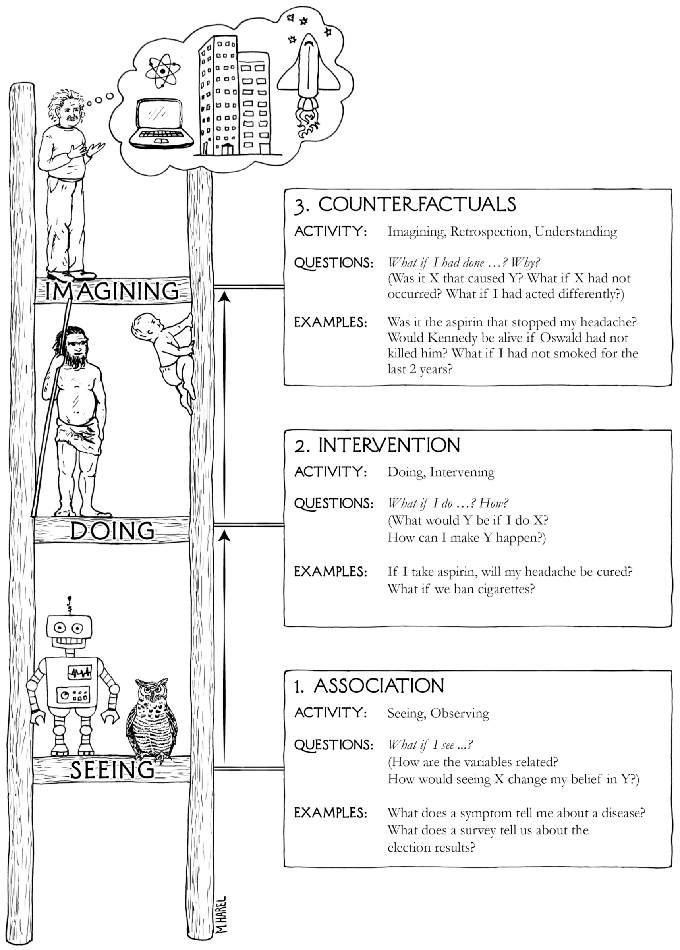
\includegraphics[width=0.3\textwidth]{images/ladder.png}
    \caption{Pearl's ladder of causality}
    \label{fig:ladder_of_caus}
\end{figure}

Q: How does causal reasoning manifest in humans? \\

A (babies): Babies less than a year old do not demonstrate causal knowledge, but do have a sense of physical continuity. \\

A (2 year olds): Can learn predictive relationships between events, but can't sponetaneously make interventions based on causal understanding. \\

A (3-4 year olds): Can infer causal maps from observing conditional dependencies. \\

A (4-5 year olds): Can make informative targeted interventions based on causal knowledge. \\

A (adolescence): Strategies for causal learning continue to improve. \\

A (adults): Evidence of an associative bias, a ``rich-get-richer" prnciple: one variable is more likely to be present if others in the causal model are also present. \\

{\bf Overall:} evidence suggests that children display ability to perform causal inference from observation (roughly consistent with Bayesian inference). More sophisticated forms of reasoning (performing novel informative interventions) come online later as a result of experience. \\

But: major deviations from rationality/good inference. \\

$\ra$ Reasons for deviations:
\begin{enumerate}
    \item Formal models of causal reasoning optimize difference cost functions.
    \item Humans do not optimize for a specific causal graph, but a flexible one.
    \item 
\end{enumerate}

{\it Takeaway:} A structured universe of tasks $\implies$ we should use structured priors. \\

{\bf Idea:} Meta Learning of causally inspired priors. Similarly to previous talks, assume a distribution of tasks, want to learn some priors that lead to sample efficient learning in new tasks. \\

Experiments: 1) learning from observations on causal networks (can the agent learn some causal structure from a DAG?); 2) learning from interventions; 3) Learning from instance specific info. \\

{\it Challenge Question:} Why does deep Rl seem to struggle with out-of-sample generalization compared to other domains? ?

Jane A: In RL, lots of ways to be out of sample (in contrast to supervised learning), so it's much harder. Generalization is just harder because lots of things can change: state, action, policy, transition function, reward, function, and so on. RL also requires an ongoing interaction with the environment -- input is really dependent on policy, so input will change as you update policy.

\subsubsection{Panel: Matt, Jane, Doina, Sergey, Karthik, Tejas, Tim}

Q: What is the role of structure vs. data? \\

Tim: Question is loaded. Depends on what you want to do: if you want to get good at a niche, specify more. If you want a general learning algorithm: specify less. \\

Tejas: Yes! The article talks about search, but to me the big question is making domains ``computable" (simulatable). The article is misguided: where do the primitives come from? Can't rely on the data to give you primitives. We should radically add structure. There are certain truths we can and should exploit to search effectively (objects, agents, physics). \\

Karthik: Humans have evolved many things over time that are key to our intelligence. Definitely having the right kind of inductive biases and structured priors to get things to work.  \\

Matt: I want to push back on that, because I hear it from psychologists. The assertion is often made that because babies have strong inductive biases, our agents have inductive biases. But its not obviously a constraint we need to fight in designing agents. I don't buy the argument that babies tell us that much. I love Rich Sutton but I think we have to start with structure (like CNNs). Also potentially a formal consideration; the abstractions we need to learn will require an arbitrarily small. \\

Doina: There's one thing to say we need only data, and there's another thing to say that we always have to learn from scratch. Right now we don't incorporate the right kind of structures so that we don't have to learn from scratch. We use some ideas (CNNs, gradient descent), but we want to avoid adding too much structure, too. \\

Jane: One thing in Rich's essay (which I agree with about 80\%) is that he said our brains/the environment are irredeemably complex. I don't agree with that. Neuroscience and cognitive science have been making great strides in understanding our brains. \\

Sergey: This question is different because of a methodological issue. ML is a mathematical/philosophical/scientific field. So, we're good at some things, but not at all. We've been great at making computer vision systems, language systems, and so on. In RL we've mostly been focused on solving some problems but that's been a proxy to a much grander vision that we hope to work. That's where the methodological flaw catches us. It's very easy to get improvement from bias in small problems. \\

Doina: I think that's true in the rest of ML too (Sergey: I didn't want to offend everyone! \dnote{tongue in cheek :)})). In NLP, yes, we can do some tasks but can't really do all tasks. In all of ML, we make tasks that are examples that help us improve algorithms/models, but ultimately we need to go to a more complex setting. \\

Matt: At the risk of engaging too much in the philosophical side of ML. We don't want to build in inductive biases that are too concentrated on one domain. In ML, we do tend to have a sense of the general domain we anticipate our agents being deployed in. We just have to make our choices about what ontology you want to buy into.\\

\spacerule

Q: We don't really know what tasks to train on in RL, especially in lifelong RL/multitask RL/meta RL. Any thoughts on defining the problem in a more precise way? \\

Doina: Simulation is obviously necessary. Think about human learning: babies have parents, who have an important role. How to build interesting and rich simulations that can be used for complex RL evaluation tasks? Well, one thing we can do is look more seriously at multi-modal data. \\

Sergey: Important to think about what RL would look like as a data driven field instead of a simulation driven field. If we don't we might be stuck in a regime where we don't think much about generalization and other core problems. We could think about RL tasks as being started with {\it data}, which is closer to the kinds of RL algorithms we might want that live in the real world. Kind of crazy to imagine an algorithm could learn a complex task {\it tabula rasa}.\\

Tejas: I agree with everything that was said. Generalization only matters when your data is limited. One way to think about that is when agents can generate their own tasks. We should think of metrics and measurements which incentivize researchers and platforms where agent can create lots of tasks, play in those tasks to learn more complex behaviors. \\

Tim: Question for Sergey: approaching RL in a data driven mode, how much of that needs to be done with real world data vs. simulation? \\

Sergey: I'll answer that with a question: what if we wanted to make a better image classifier? We do it with real data in vision because it's easier to make progress. So, in RL, it's easier too, because of the inherent complexity/diversity in the real data. \\

Doina: Bit of a different problem b/c we need trajectories. Lots of trajectories. Trajectories generated by people might be very different too. Might be really hard to understand/learn from whole trajectories. \\

Sergey: Might not be that hard. Can collect lots of self driving car data, grasping data, and so on, relatively easily. \\

Jane: Tend to agree with you (Sergey). One question about real data: can we make guarantees about moving beyond that labratory data? \\

Sergey: That's where you need to be really careful. \\

Tejas: from first principles, no reason we can't make a simulator that's indistinguishable in terms of graphics and physics. Just a matter of time before we have a simulator that can replace real world data. \\

Sergey: Sure! But might be really slow. Why wait? \\

\spacerule

Q: What's the main reason to used model-based vs. model-free learning? \\

Karthik: Learning a model of the world can give you far more flexibility about what you can accomplish. In model free learning, you tend to just have on policy/value function, it wont generalize well/transfer across tasks. Can cover roughly 90\% of things that can happen with a (good) model. \\

Doina: Not so sure the distinction is salient. Models can be thought of as generalized value functions, where things become much more blurry. Might end up with model-based RL that is much less efficient because learning the mapping from obserbation to observation is very hard. To do this, need to understand the effects of your actions vs. understand what other variables are important for policy/value function. This latter component might be much simpler than the former. Might need to rethink the nature of our models. We should build models that are small bricks. \\

Matt: That resonates! Fascinated by grey the distinction is between model-free and model-based. For a number of years in neuroscience this distinction was treated as very categorical. But, we've realized it's much messier. 





% ------------
% -- Monday --
% ------------
\newpage
\section{Tuesday May 7th: Main Conference}
Onto day two! Today is entirely the main conference. I have a lot of meetings today so I will only be around for a few talks, sadly. 


\subsection{Keynote: Emily Shuckburgh on ML Conducting a Planetary Healthcheck}

Remember: NOLA in 2005 post Katrina. We thought this would be a wake up call. \\

CO$_2$ in the atmosphere in 2005: 378 parts per million, in 2019; CO$_2$ 415 parts per million. Hurricanes and cyclones in Mumbai, rising seas, wetter skies $\implies$ devastation caused by these events is that much worse. \\

{\bf Note:} One {\it million} species at risk of extinction in the next decades (from a recent study on biodiversity). \\

$\ra$ We are having a huge impact on our planet. \\

\dbox{{\bf Guiding Question:} How can we get a sense of the health of our planet, and turn it around? Can we use Machine Learning to make that happen?}

\subsubsection{Challenges for ML in Climate Science}

Key questions, observations, and action items:
\begin{enumerate}
    \item Urgently need actionable information on climate risk
    
    Need to understand potential risk and outcomes from
    \begin{enumerate}
        \item Flooding, heat waves, and other disasters.
        \item Effects of changes in biodiversity.
        \item Impact on supply chains (food, water, and beyond), and 4) effects on the natural world (coral reefs, forests, arctic sea ice, permafrost).
    \end{enumerate}
    
    \item We have vast data-sets describing how the planet is changing.
    
    Includes data from satellites, robotic instruments under water, networked sensors, massive computer simulations, crowd sourcing.
    
    $\ra$ We have more data than we know what to do with.
    
    \item {\bf Main Point:} Can we employ advances in data science and machine learning to harness this data (from 2.) to help address the challenges in (1.)?
    
\end{enumerate}

\begin{figure}[h!]
    \centering
    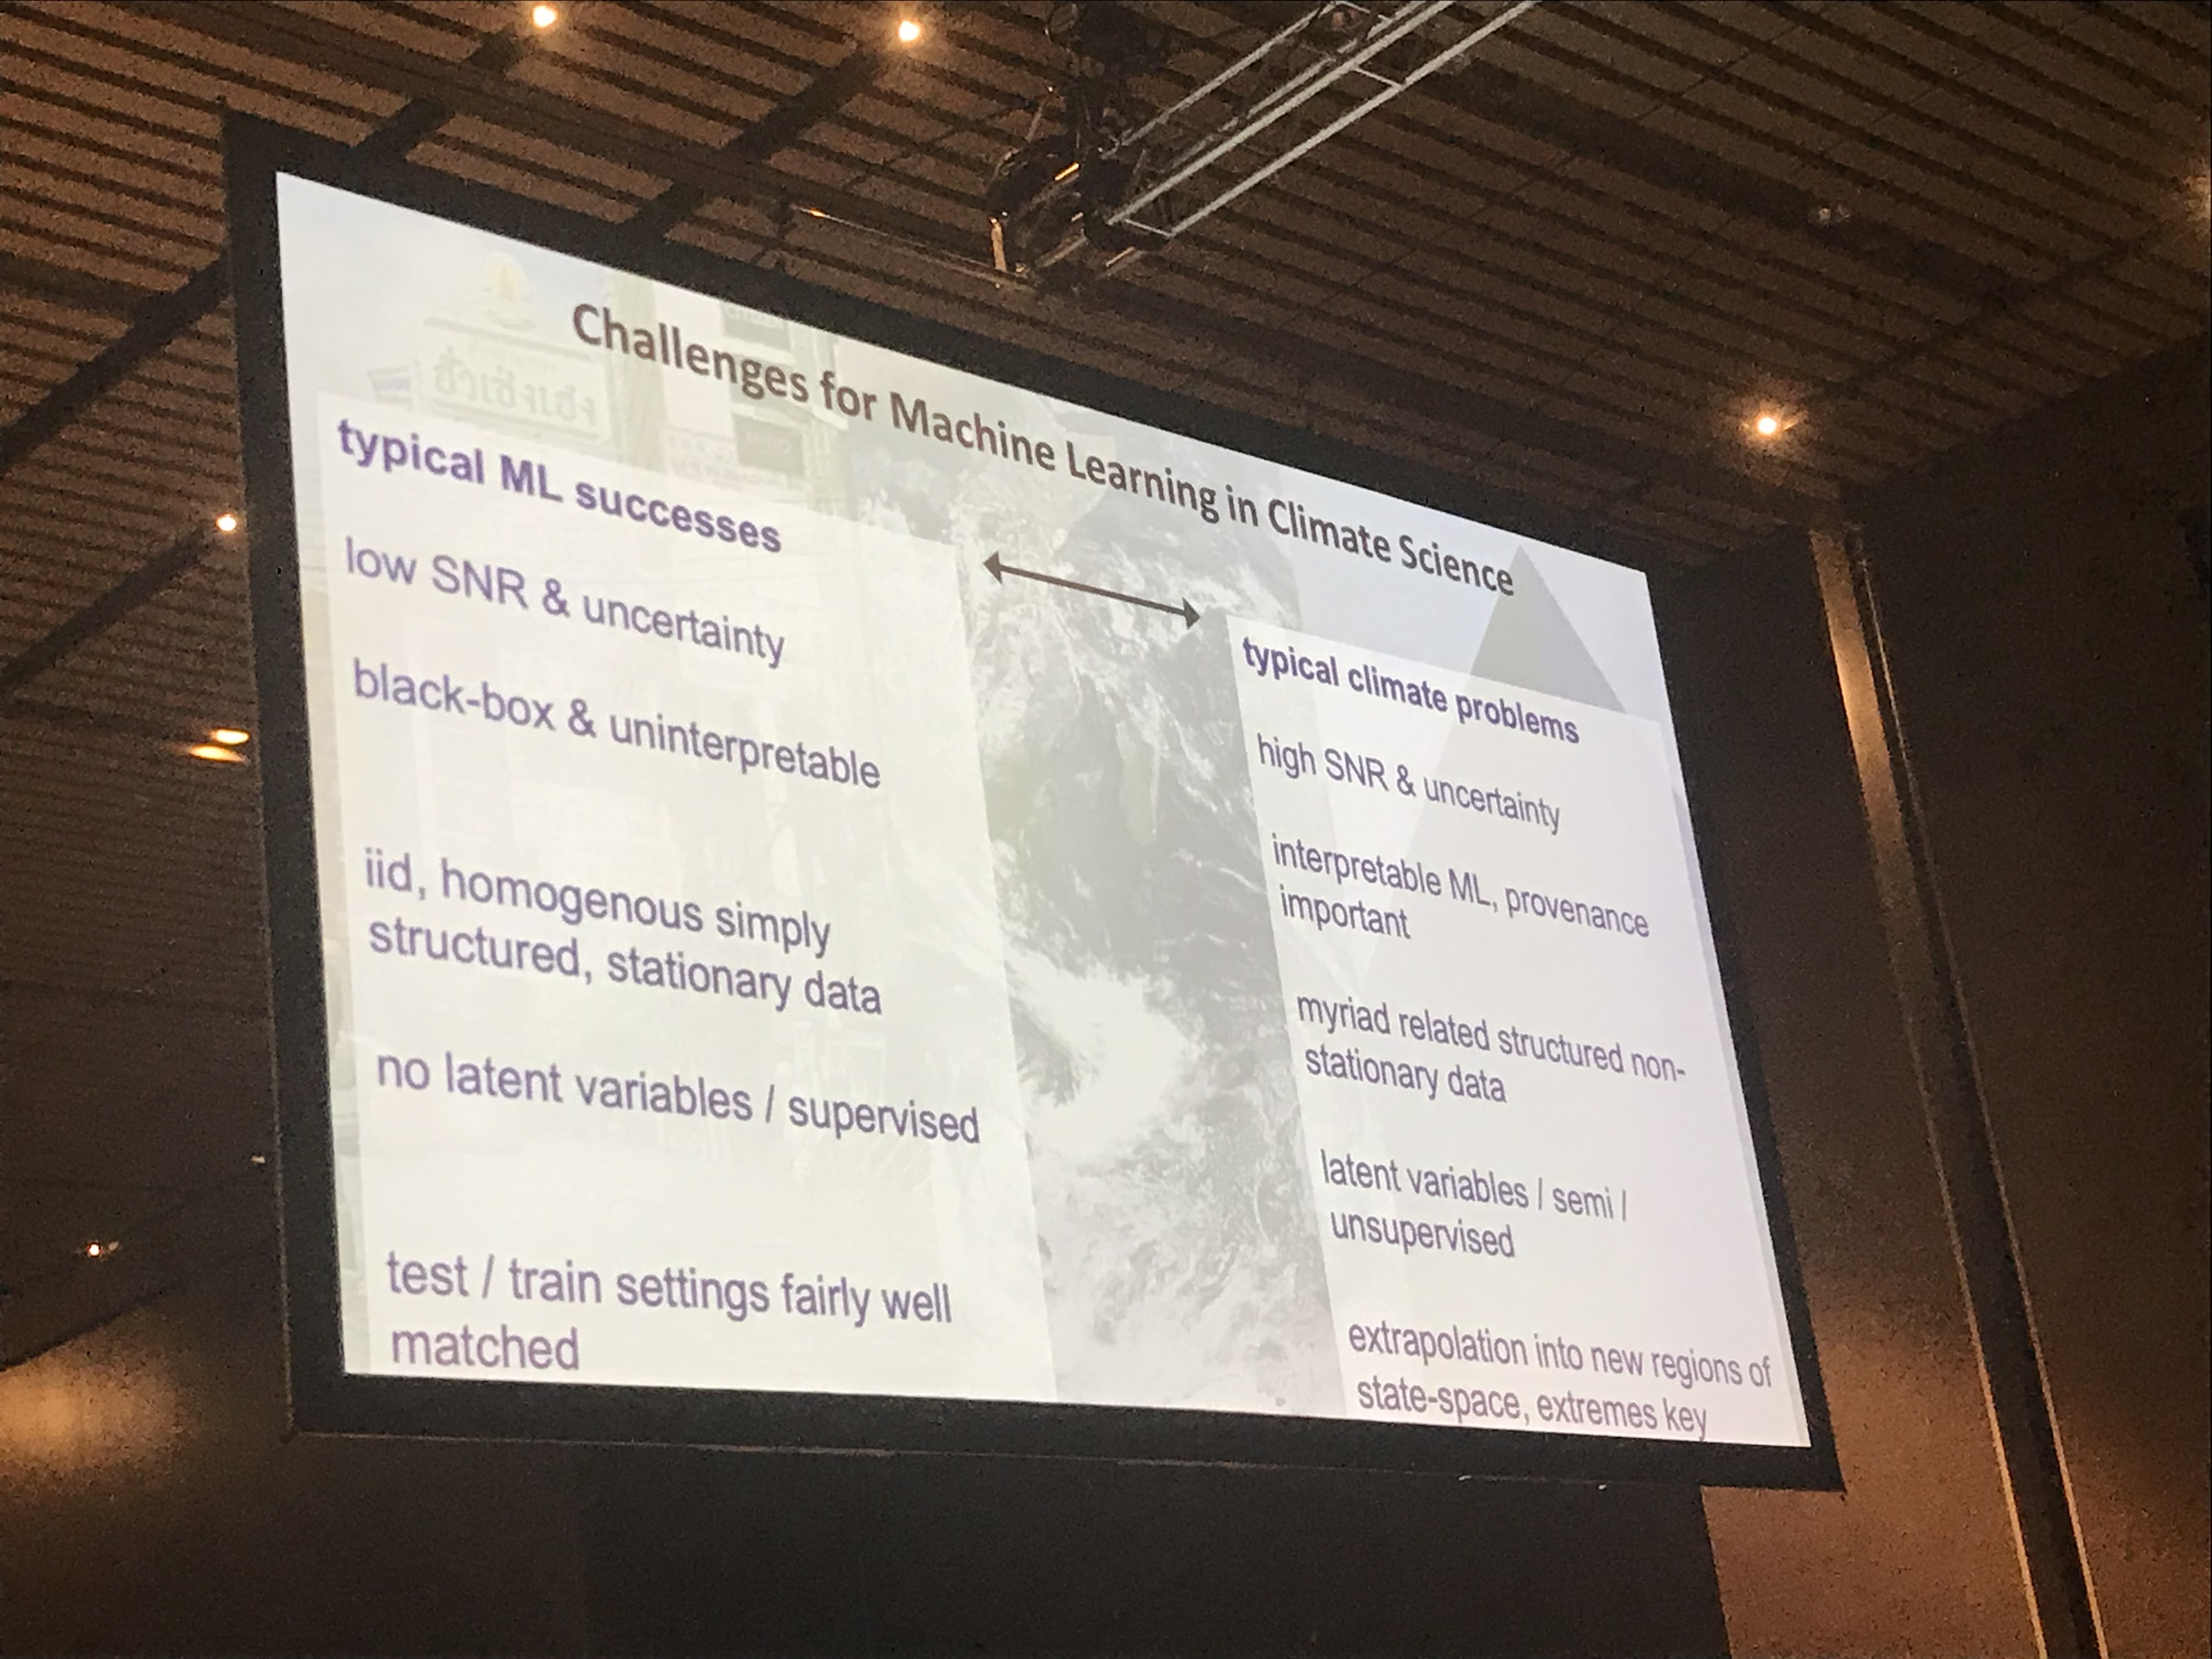
\includegraphics[width=0.4\textwidth]{images/cc_challenges.JPG}
    \caption{Challenges in bringing tools from ML to bear on problems in Climate Science.}
    \label{fig:cc_ml}
\end{figure}

Q: In spite of the challenges (see Figure~\ref{fig:cc_ml}), what can we do? \\

A: Three steps to conduct a planetary healthcheck:
\begin{enumerate}
    \item Monitoring the planet
    \item Treating the symptoms
    \item Curing the disease
\end{enumerate}

\subsubsection{Step One: Monitoring The Planet}

Q: How can we appropriately monitor the health of the planet? It's a huge challenge! Lots of important data is sparse, while less important (or low signal-noise ratio data) is abundant. \\

A: More comprehensive testing -- not just temperature, but lots of other properties, too.

\begin{figure}
    \centering
    \subfloat[Surface temperature over time]{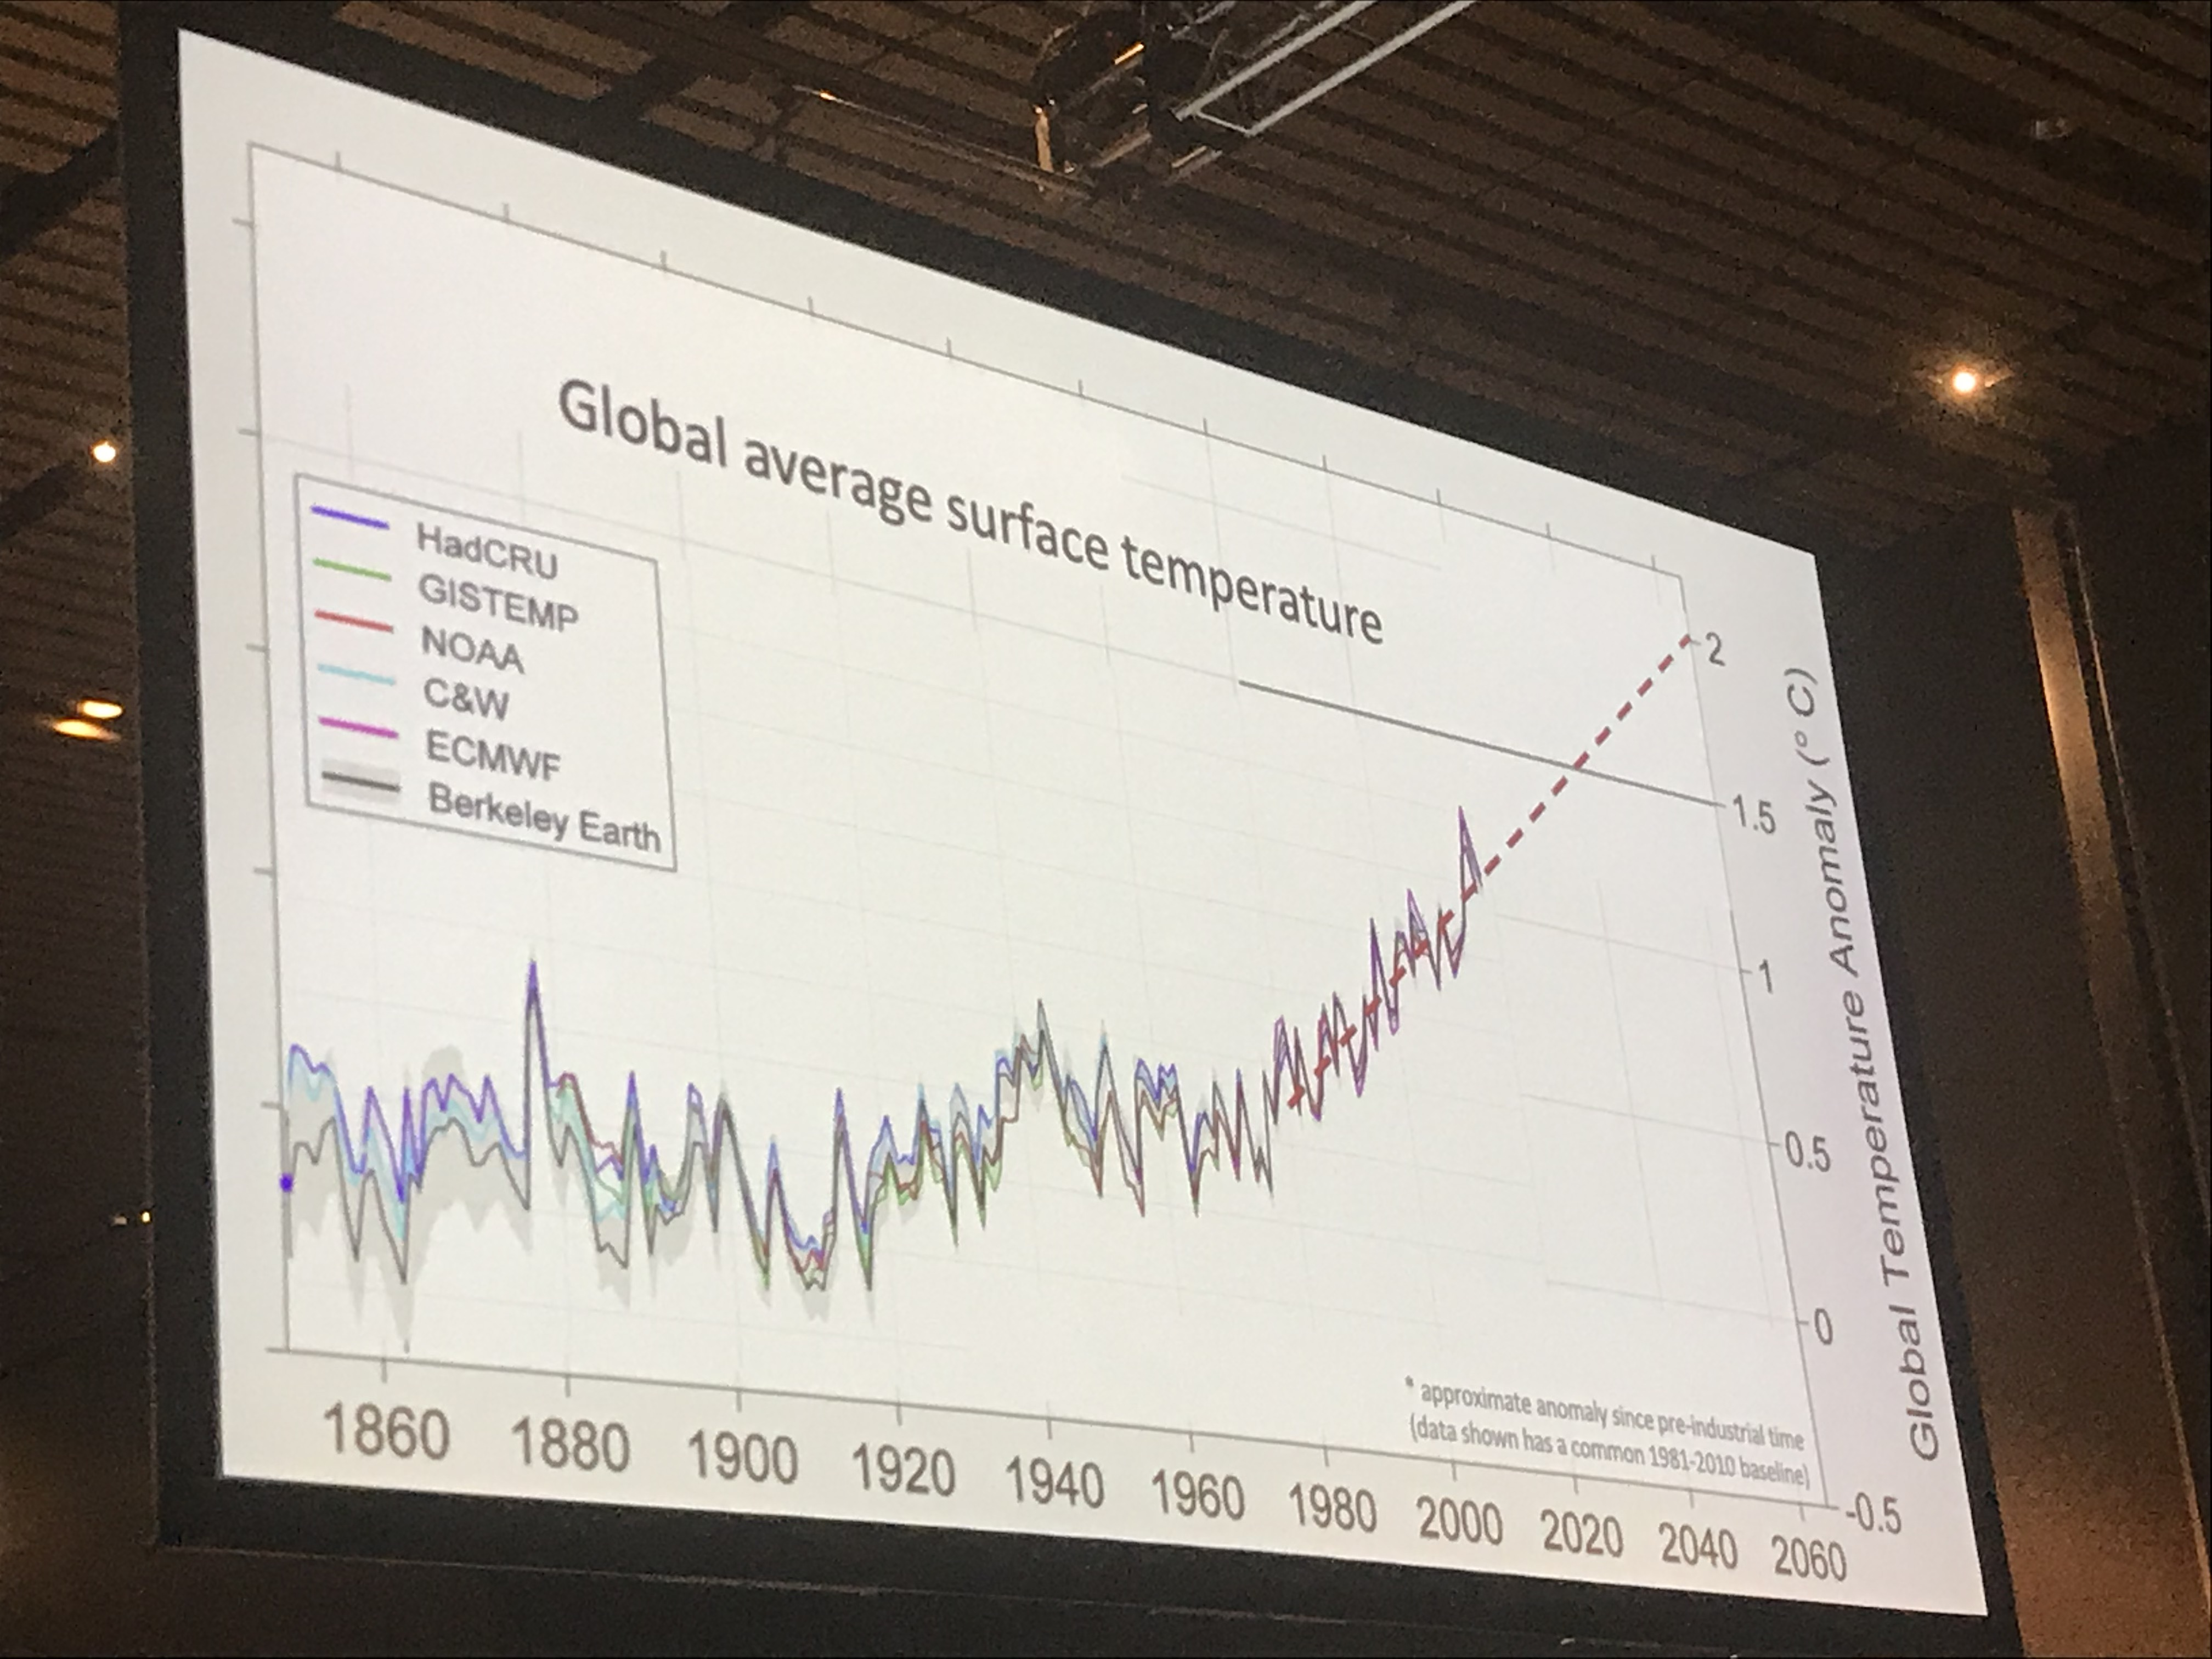
\includegraphics[width=0.4\textwidth]{images/temp.JPG}} \hspace{5mm}
    \subfloat[Other climate-relevant data over time]{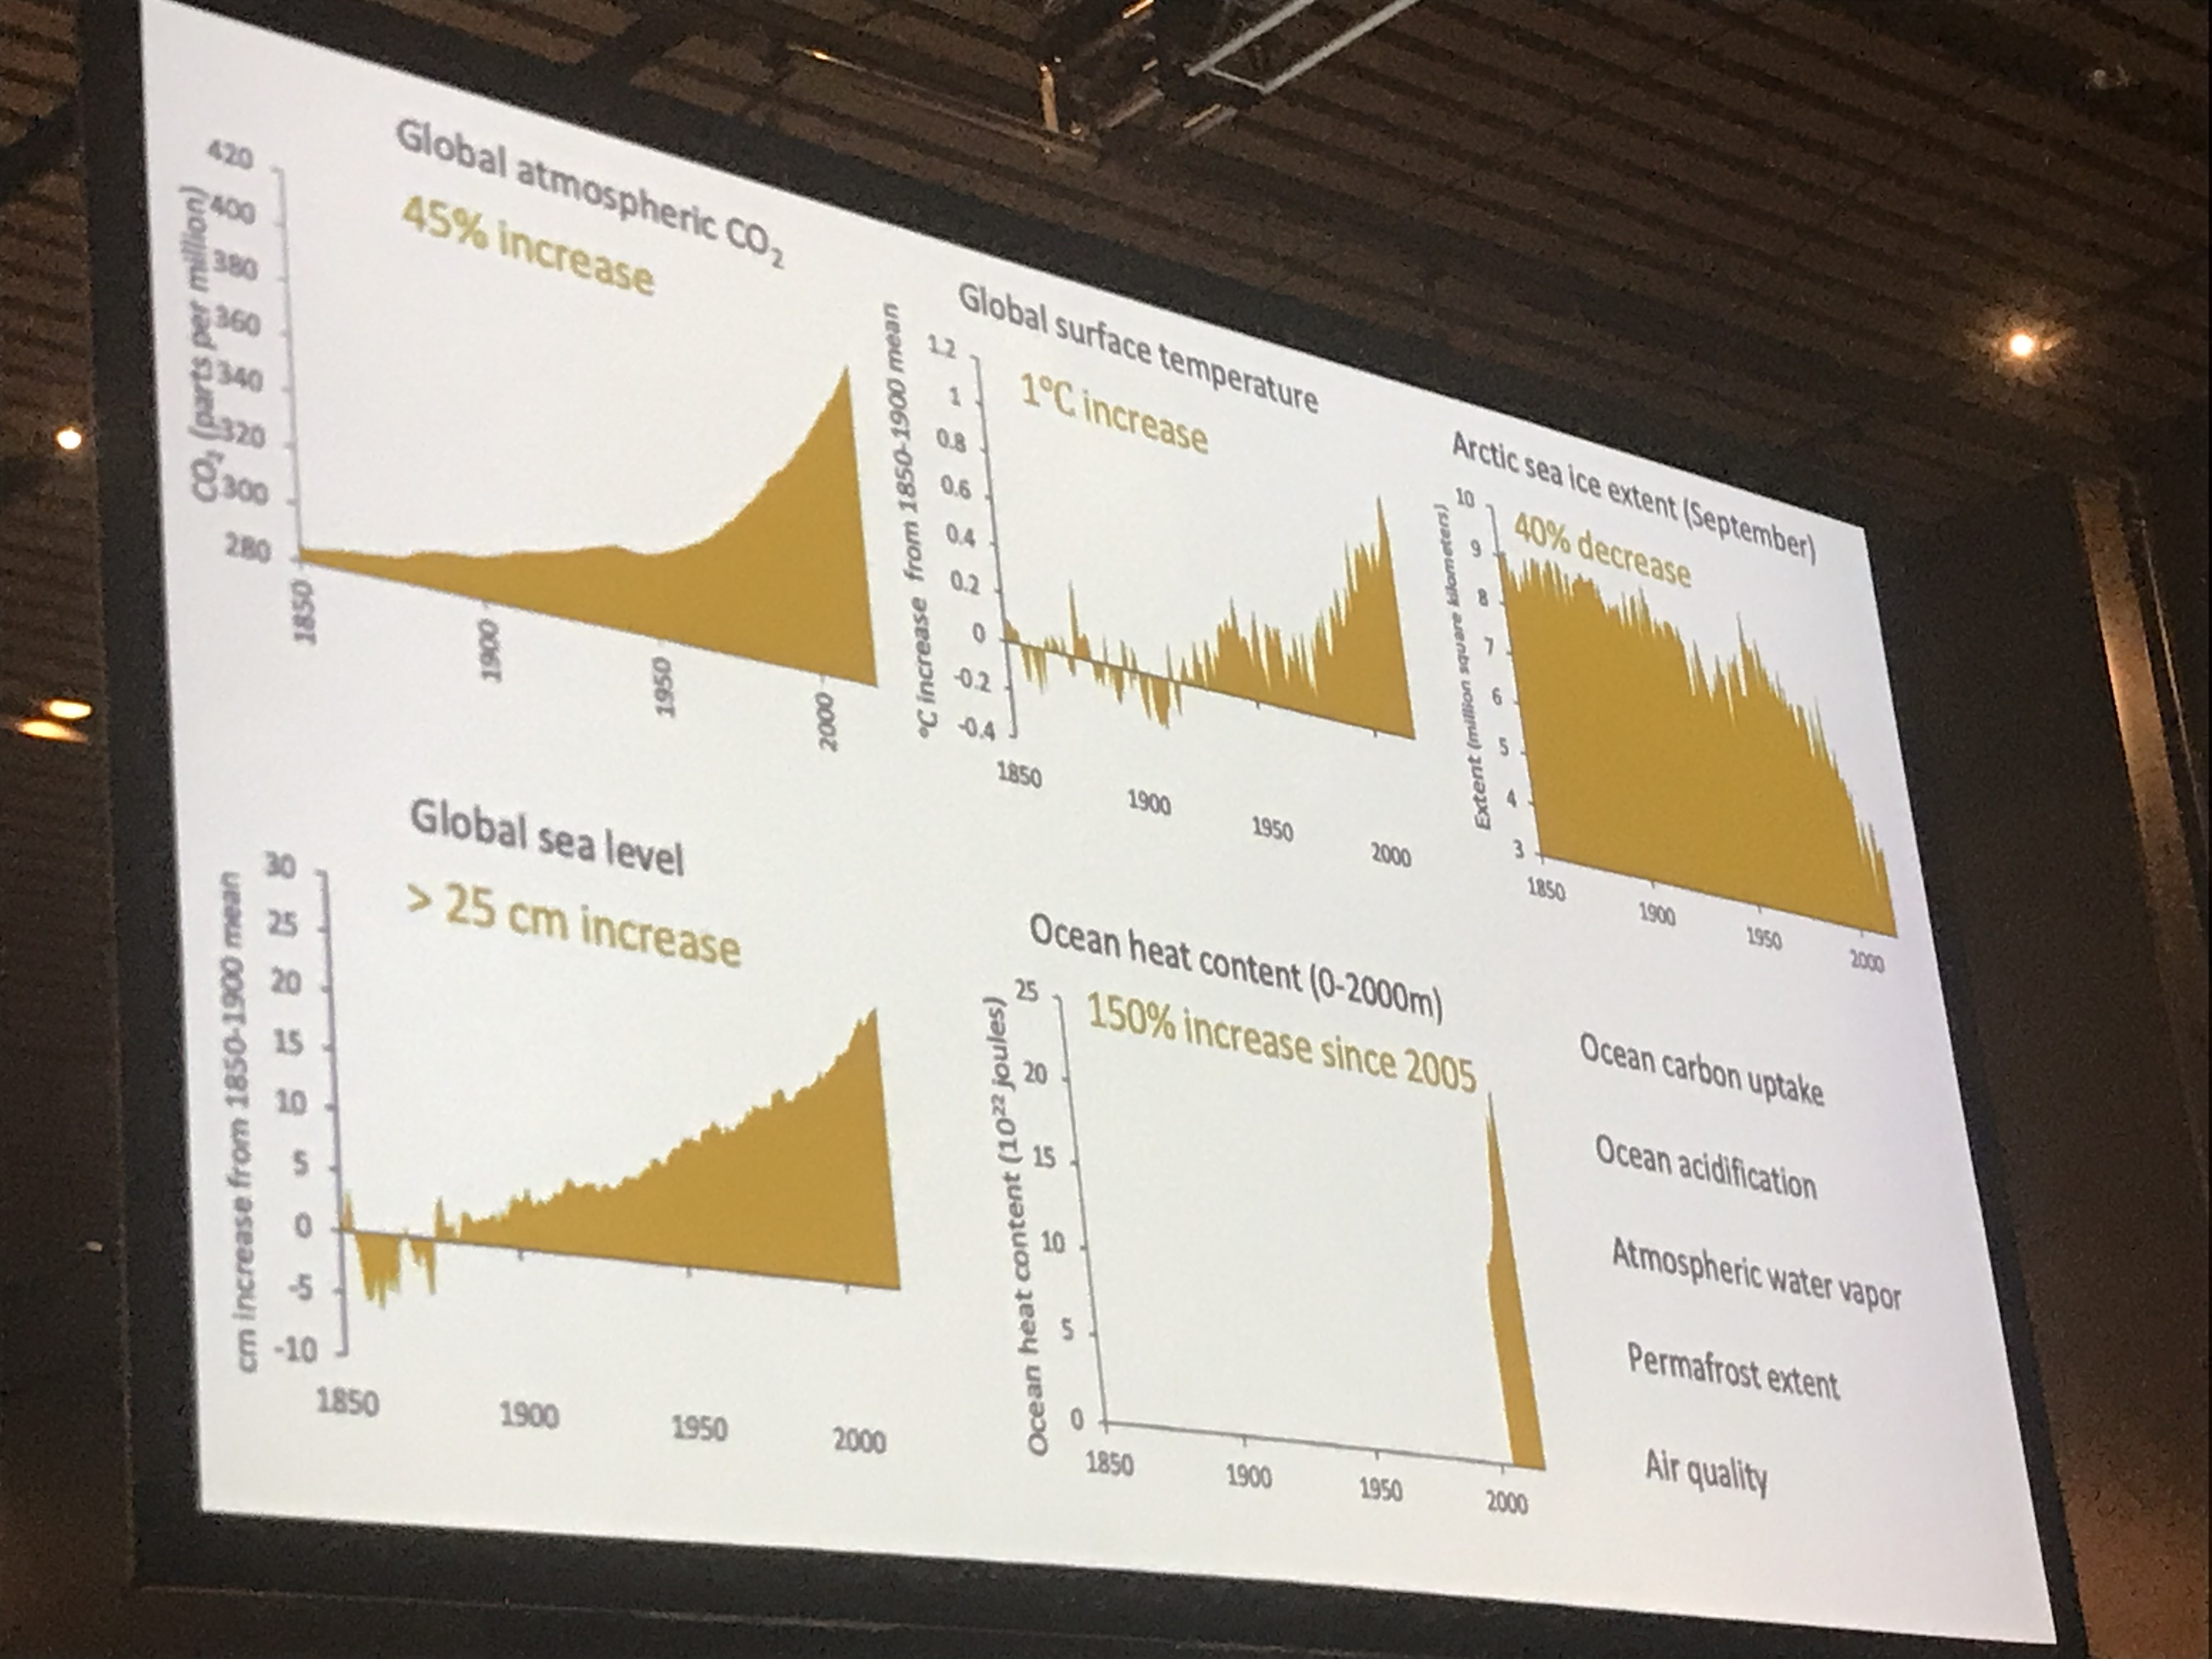
\includegraphics[width=0.4\textwidth]{images/cc_data.JPG}}
    \caption{Changes in properties of the earth's health over time.}
    \label{fig:cc_data}
\end{figure}


\subsubsection{Step Two: Treating the Symptoms}

Standard tools: co-ordinated international climate modeling project (CMIP6): \~ 40 Petabytes. Around a million lines of code, used to run simulations of surface radiation, changes in solar radiation, and so on. \\

Q: What do these models do for us? \\

A: They make predictions about critical properties in the future, like emissions due to greenhouse gases with and without different interventions, and so on. \\

$\ra$ we can actually predict global average surface temperature extremely well. \\

Q: What will future conditions be like in the world's cities and megacities? How can we predict these things? \\

A: clime models can project these changes many years into the future! \\

But: 1) have coarse resolution, 2) have systematic biases at a local level, and 3) different clime models do better/worse at representing different aspects of the climate system. \\

Example: Consider a climate model making predictions about temperatures in London. \\

$\ra$ Sometimes, the model is systematically wrong (biased). It's too high for long periods, then too low, and so on. So how can we remedy this? \\

{\bf Approach:} Apply probabilistic machine learning to build a new predictive model from actual observed weather data. That is, learn $f : \mc{X} \ra \mc{Y}$, given lots of weather data. \\

Q: Can we go further? Can we extend this model to account for correlated risks and map to data on impacts? \\

$\ra$ Really we'd like to regulate sustainable urban drainage, thermal comfort in buildings, and address questions like how vulnerable a particular country/region is to clime disruption? \\

Similar approach---consider a task where: \\
\hspace{8mm}{\bf input:} time, space, climate model outputs, meteorological data
\hspace{8mm}{\bf output}: future risk of specific impact occurring, with the {\bf task:} of synthesizing and interpolating different datasets, learn mappings between different variables, may need to find novel sources of data.\\

\subsubsection{Step Three: Cure the Disease}

{\bf Key Takeaway:} many opportunities for improve future projections of climate change to inform policymaking. Here are a few:

\begin{enumerate}
    \item Blend data-driven and physics based approaches
    
    $\ra$ Can combine physics models of ice melt and machine learning models (with our large dataset) to make more accurate predictions of ice melt.
    
    \item Develop data-based simulators of key processes
    
    $\ra$ Given massive datasets of key processes, such as cloud formations, we can help to build more accurate models. Current climate models don't scale well, so we need to find new ways to model climate change.
    
    \item Use ML to better understand the {\it physical processes} involved in key shifts, as in glacier shifts (see Figure~\ref{fig:glacier}.
    
\end{enumerate}

\begin{figure}
    \centering
    \subfloat[]{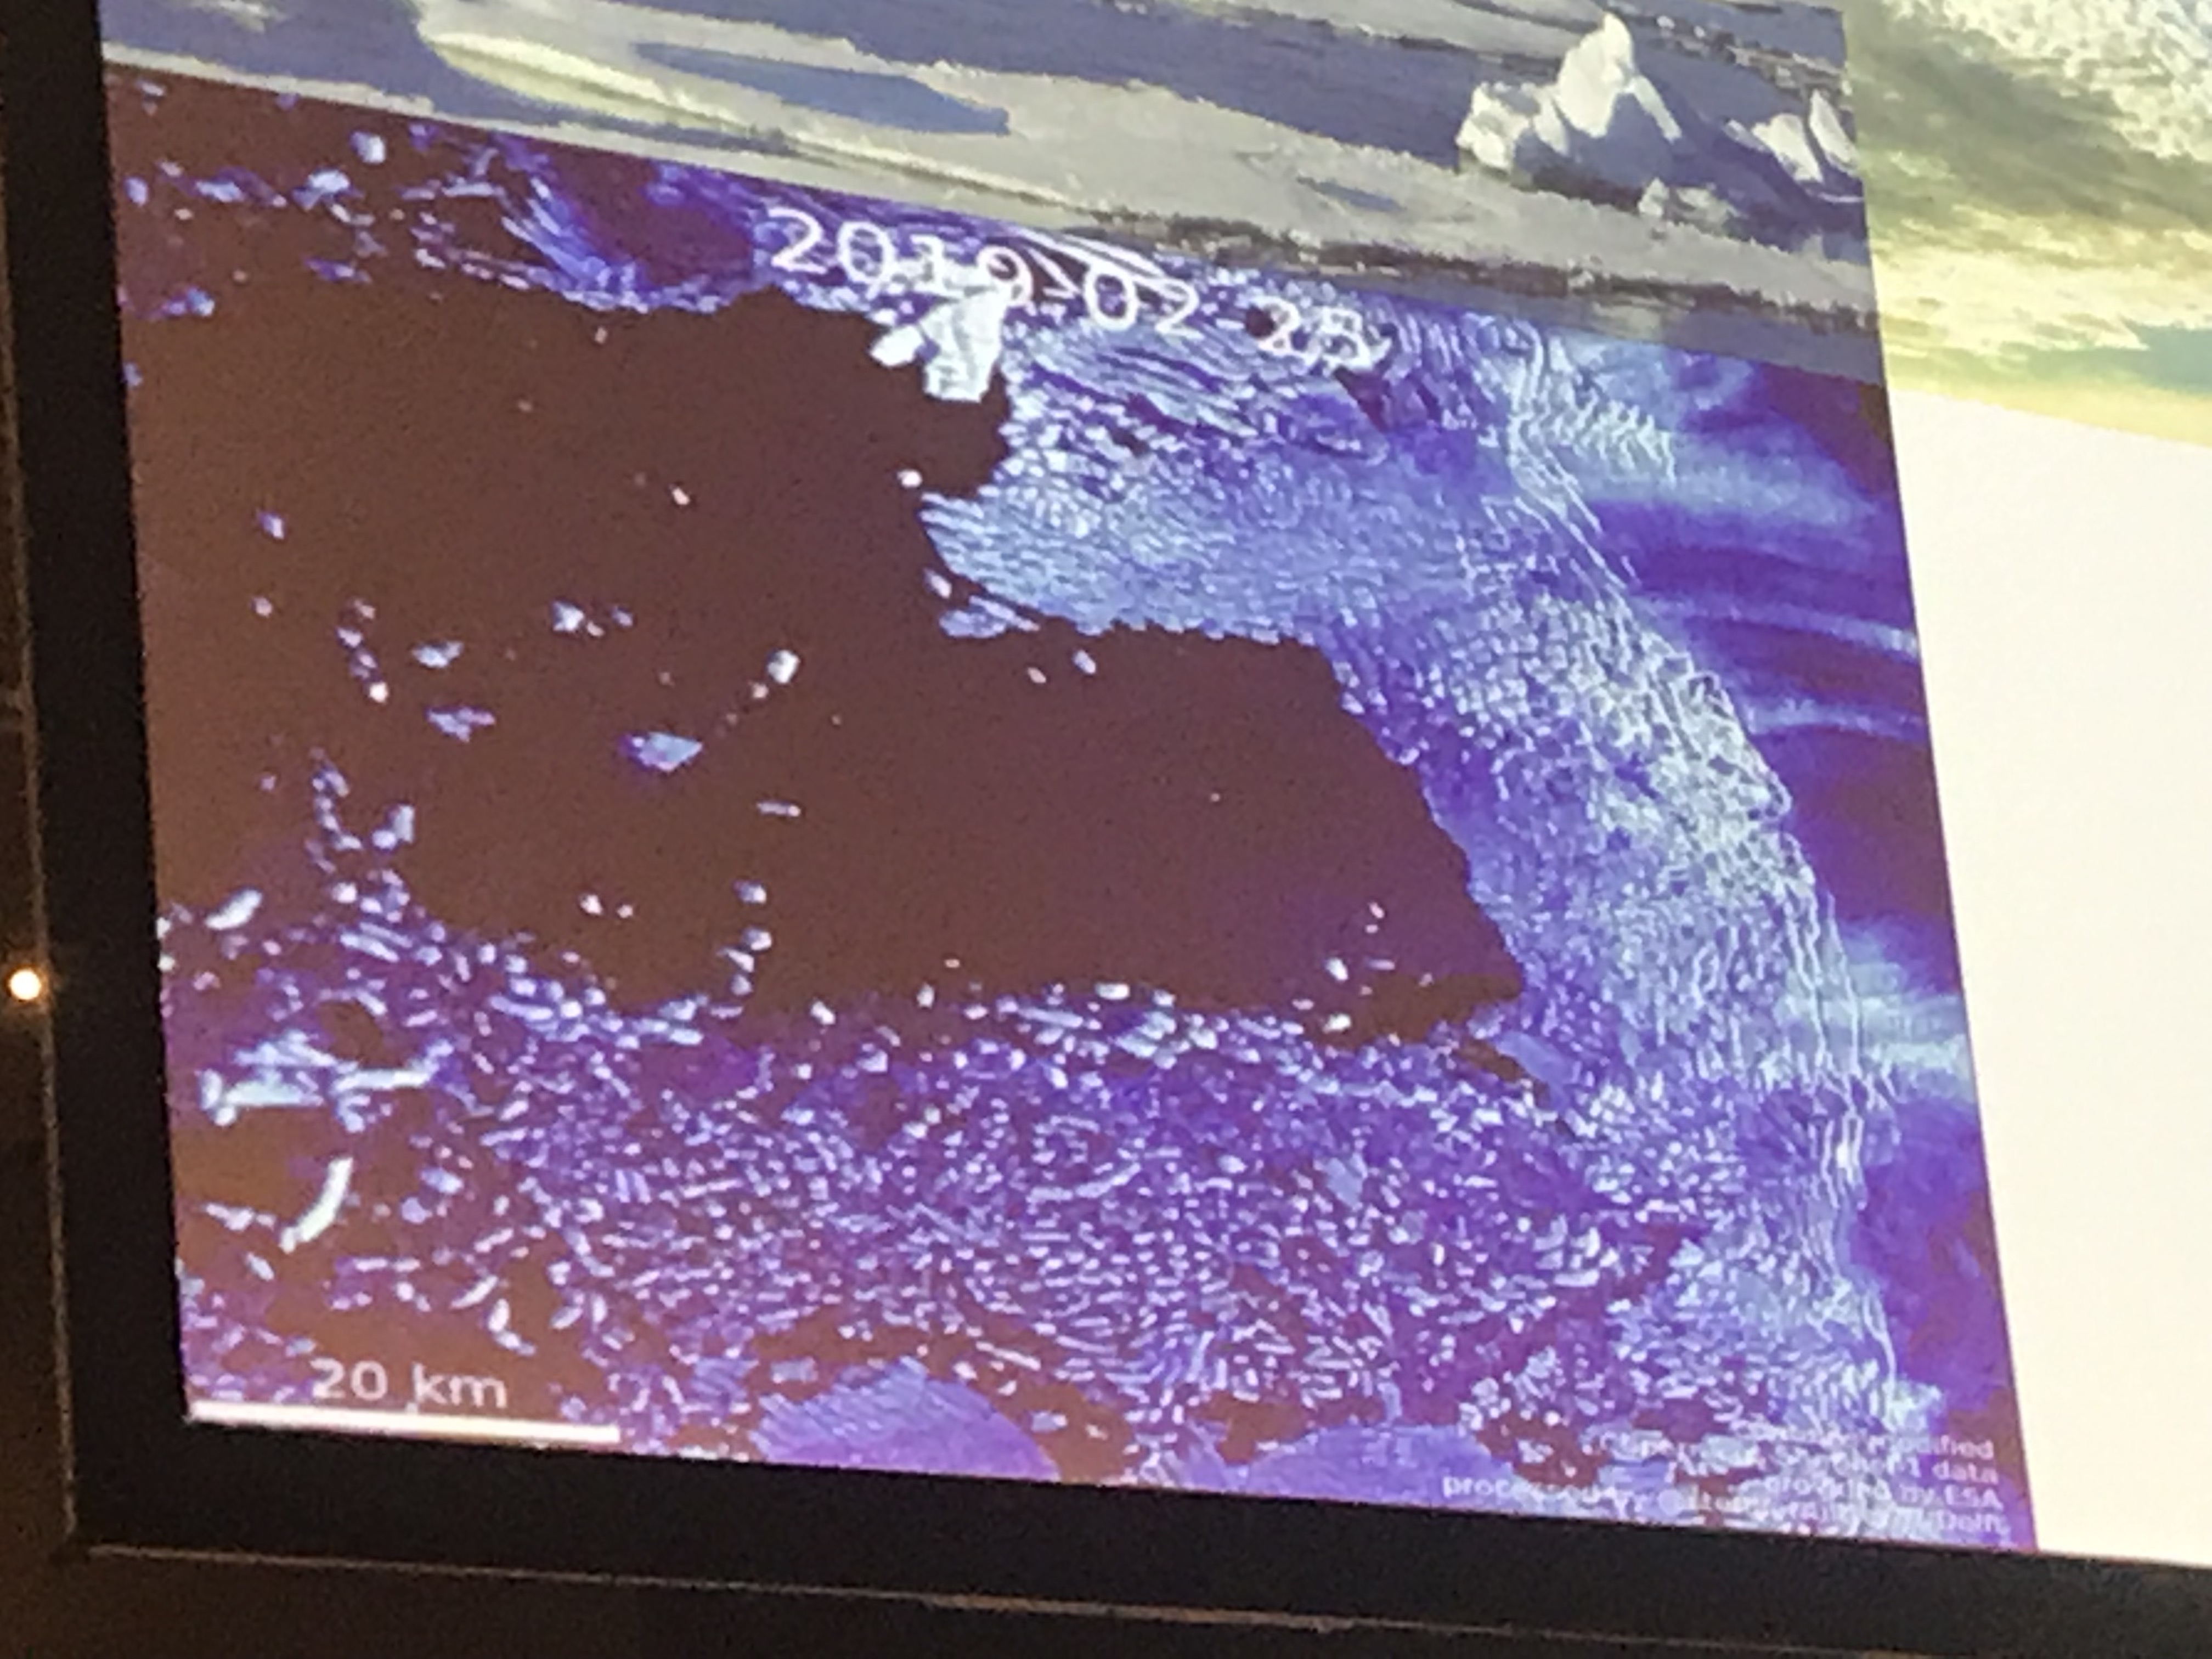
\includegraphics[width=0.29\textwidth]{images/glacier_1.JPG}} \hspace{3mm}
    \subfloat[]{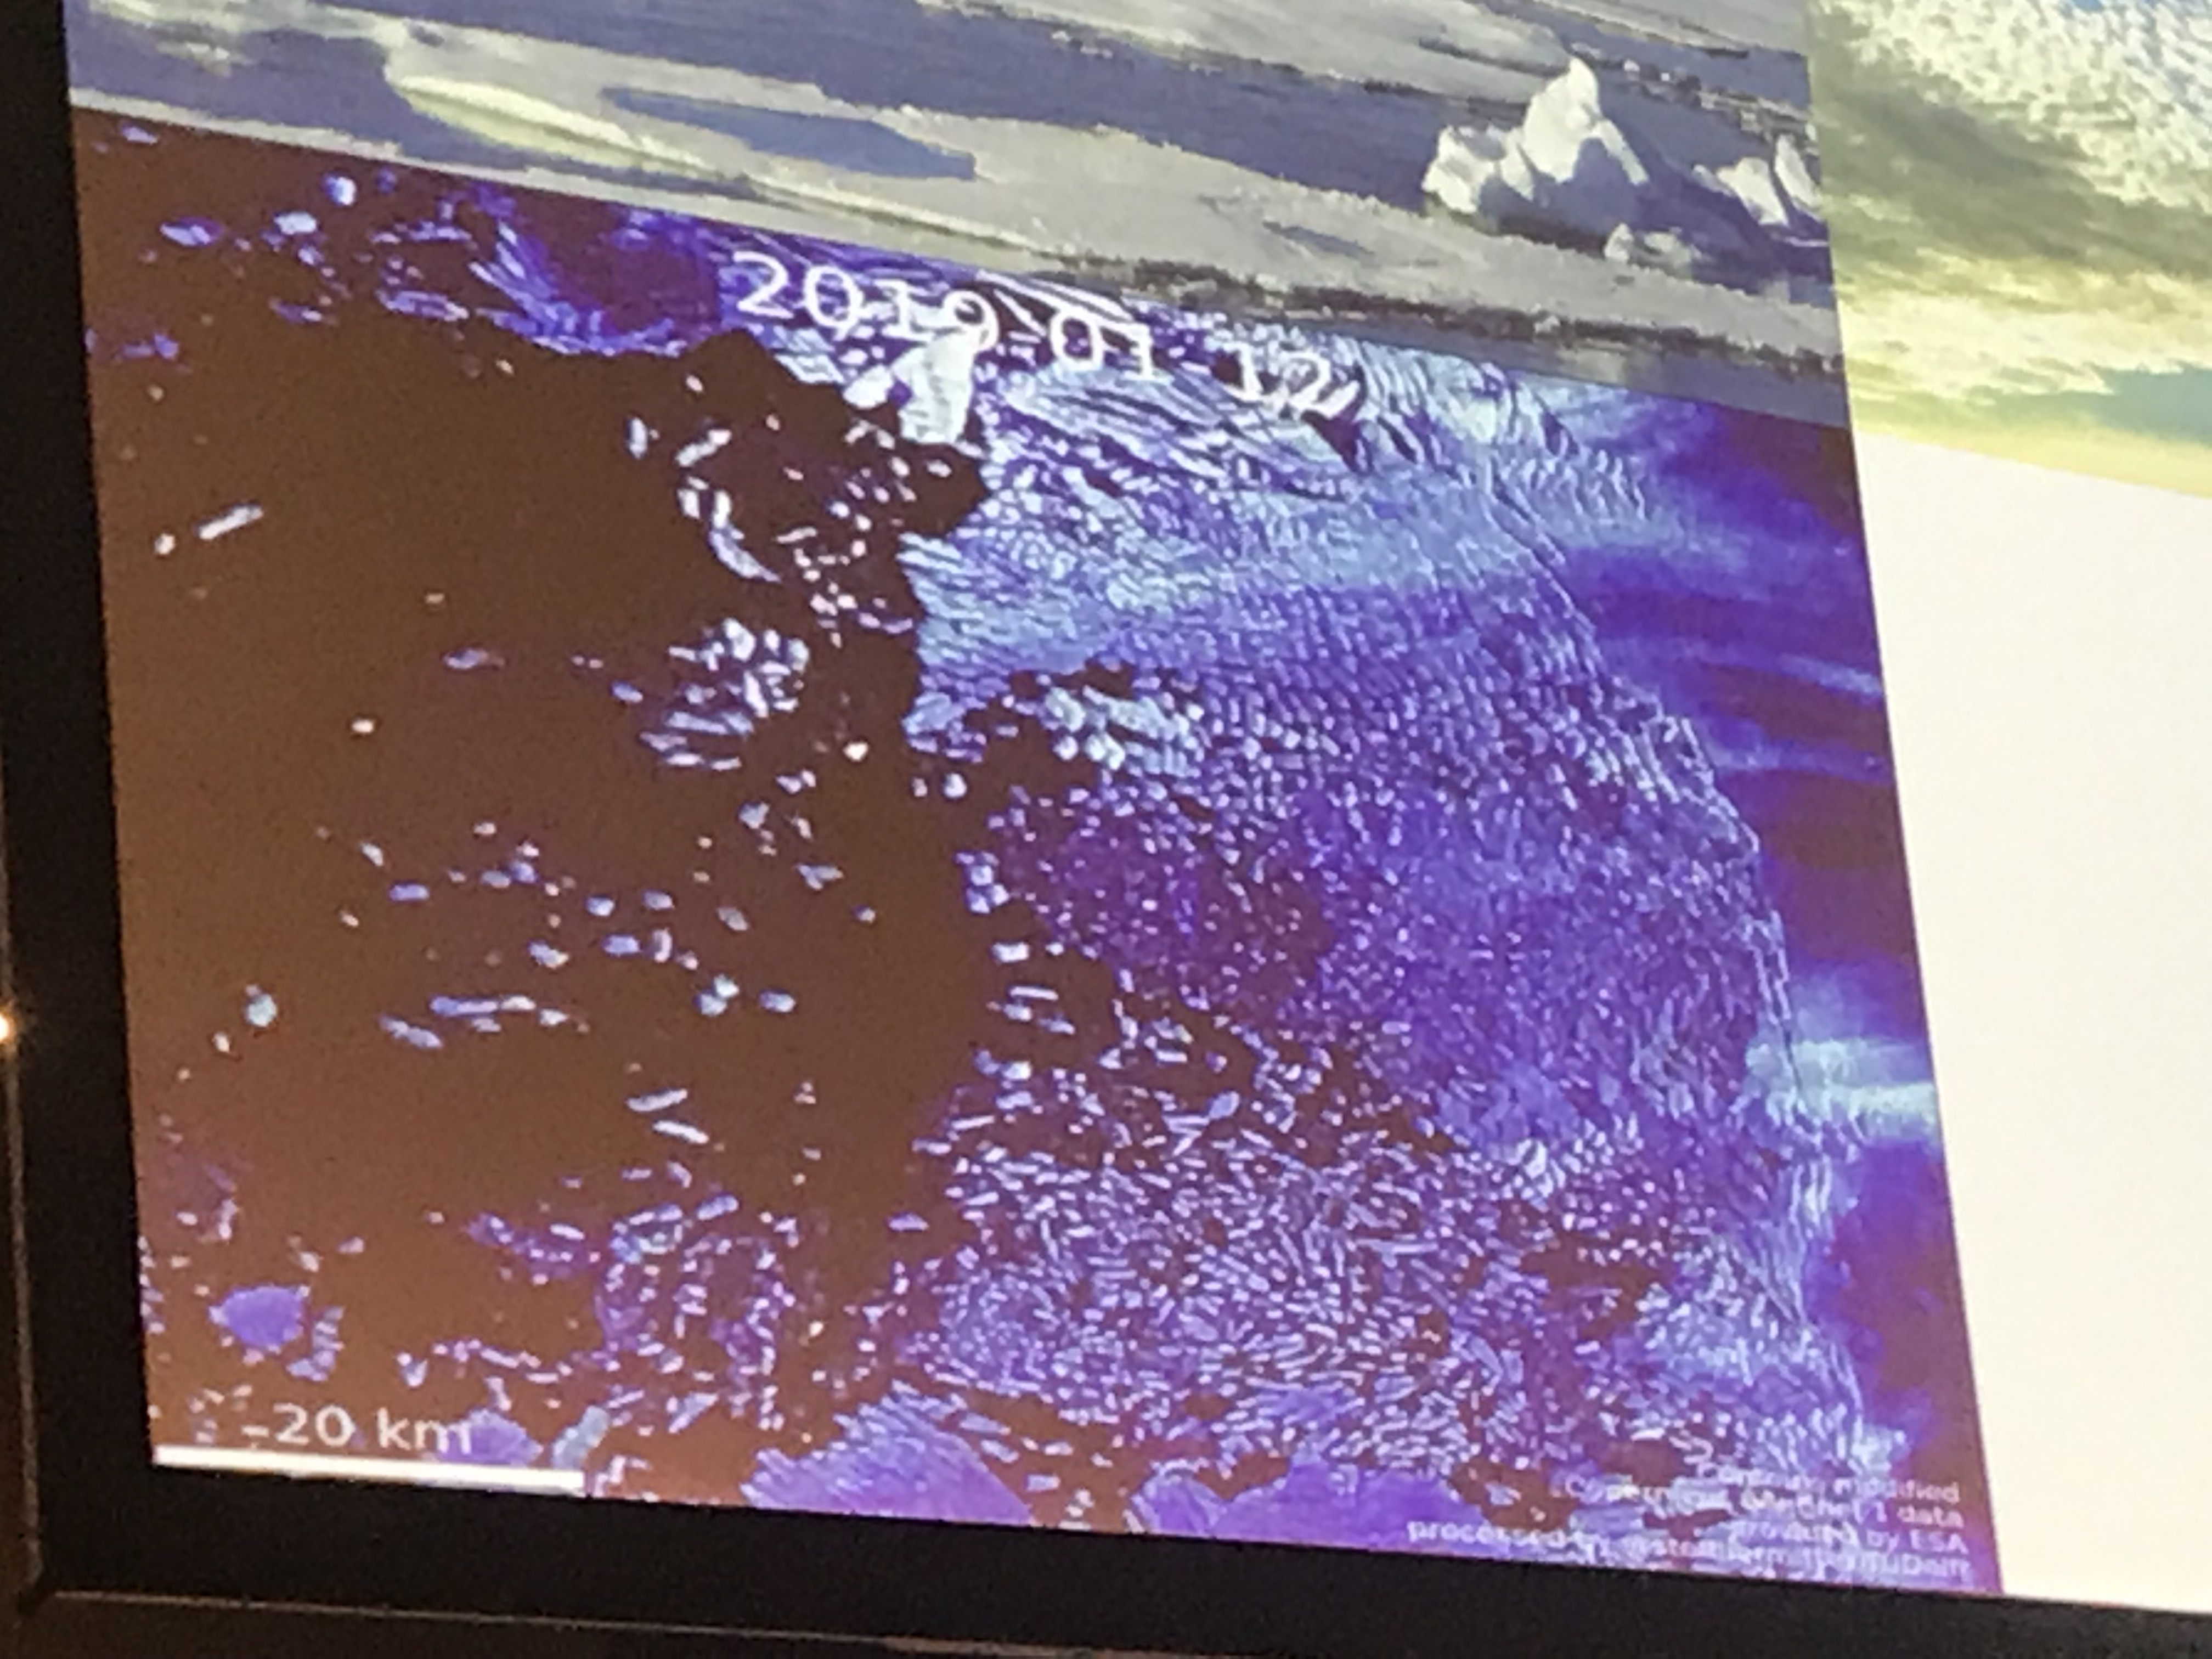
\includegraphics[width=0.29\textwidth]{images/glacier_2.JPG}} \hspace{3mm}
    \subfloat[]{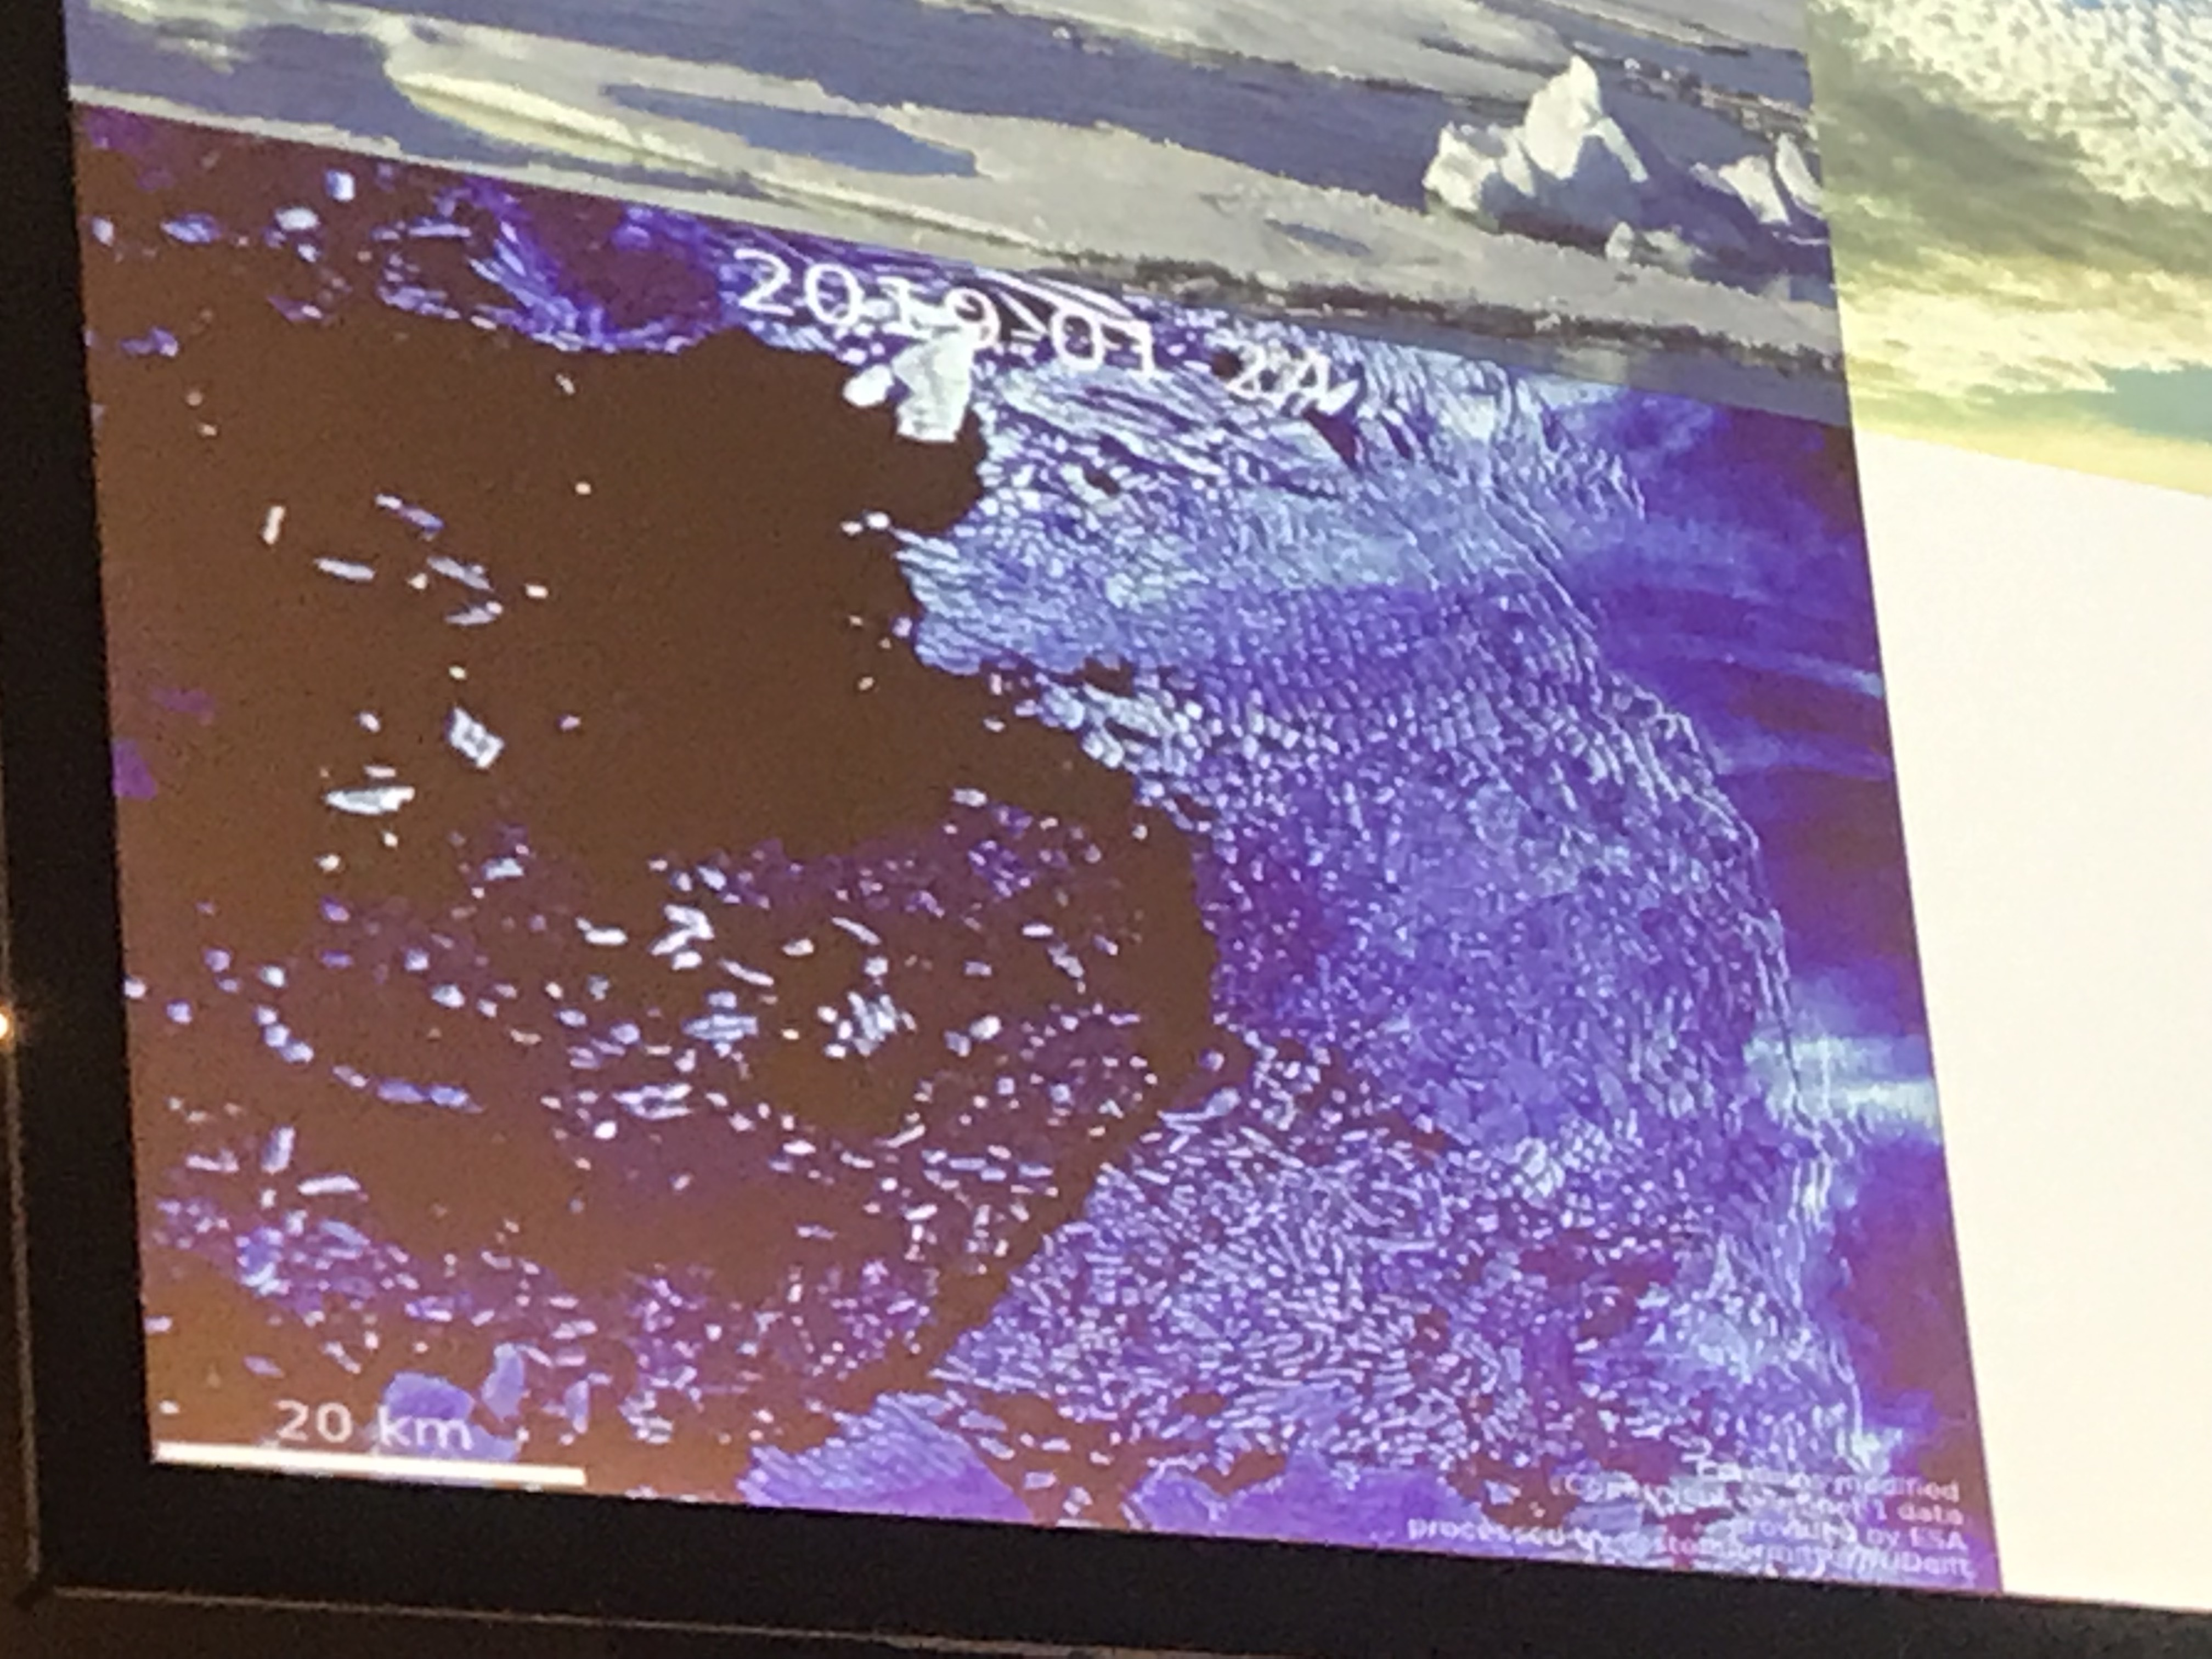
\includegraphics[width=0.29\textwidth]{images/glacier_3.JPG}} \hspace{3mm}
    \caption{Change in glacial structure over time.}
    \label{fig:glacier}
\end{figure}

Summary:
\begin{enumerate}
    \item Climate change is perhaps the defining issue of our time
    \item To assess risks posed to society and the natural world, we need more information and tools.
    \item Vast datasets cover every aspect of the planet's health but we lack some of the {\it tools} tp process them to generate that information.
    
    \item {\bf Takeaway Question:} Can we establish benchmark tasks that drive climate research forward much like ImageNet has done for vision?
\end{enumerate}

\dnote{Stepping out for meetings the rest of the day, back at it tomorrow!}



% ------------
% -- Tuesday --
% ------------
\newpage
\section{Wednesday May 8th: Main Conference}
Today I should be around for more talks. The day begins with a keynote!

\subsection{Keynote: Pierre-Yves Oudeyer on AI and Education}

{\bf Note:} Children are extraordinary learners! And typically do so without an engineer following them hand tuning every aspect of their learning algorithm and environment. \\

\begin{figure}[h!]
    \centering
    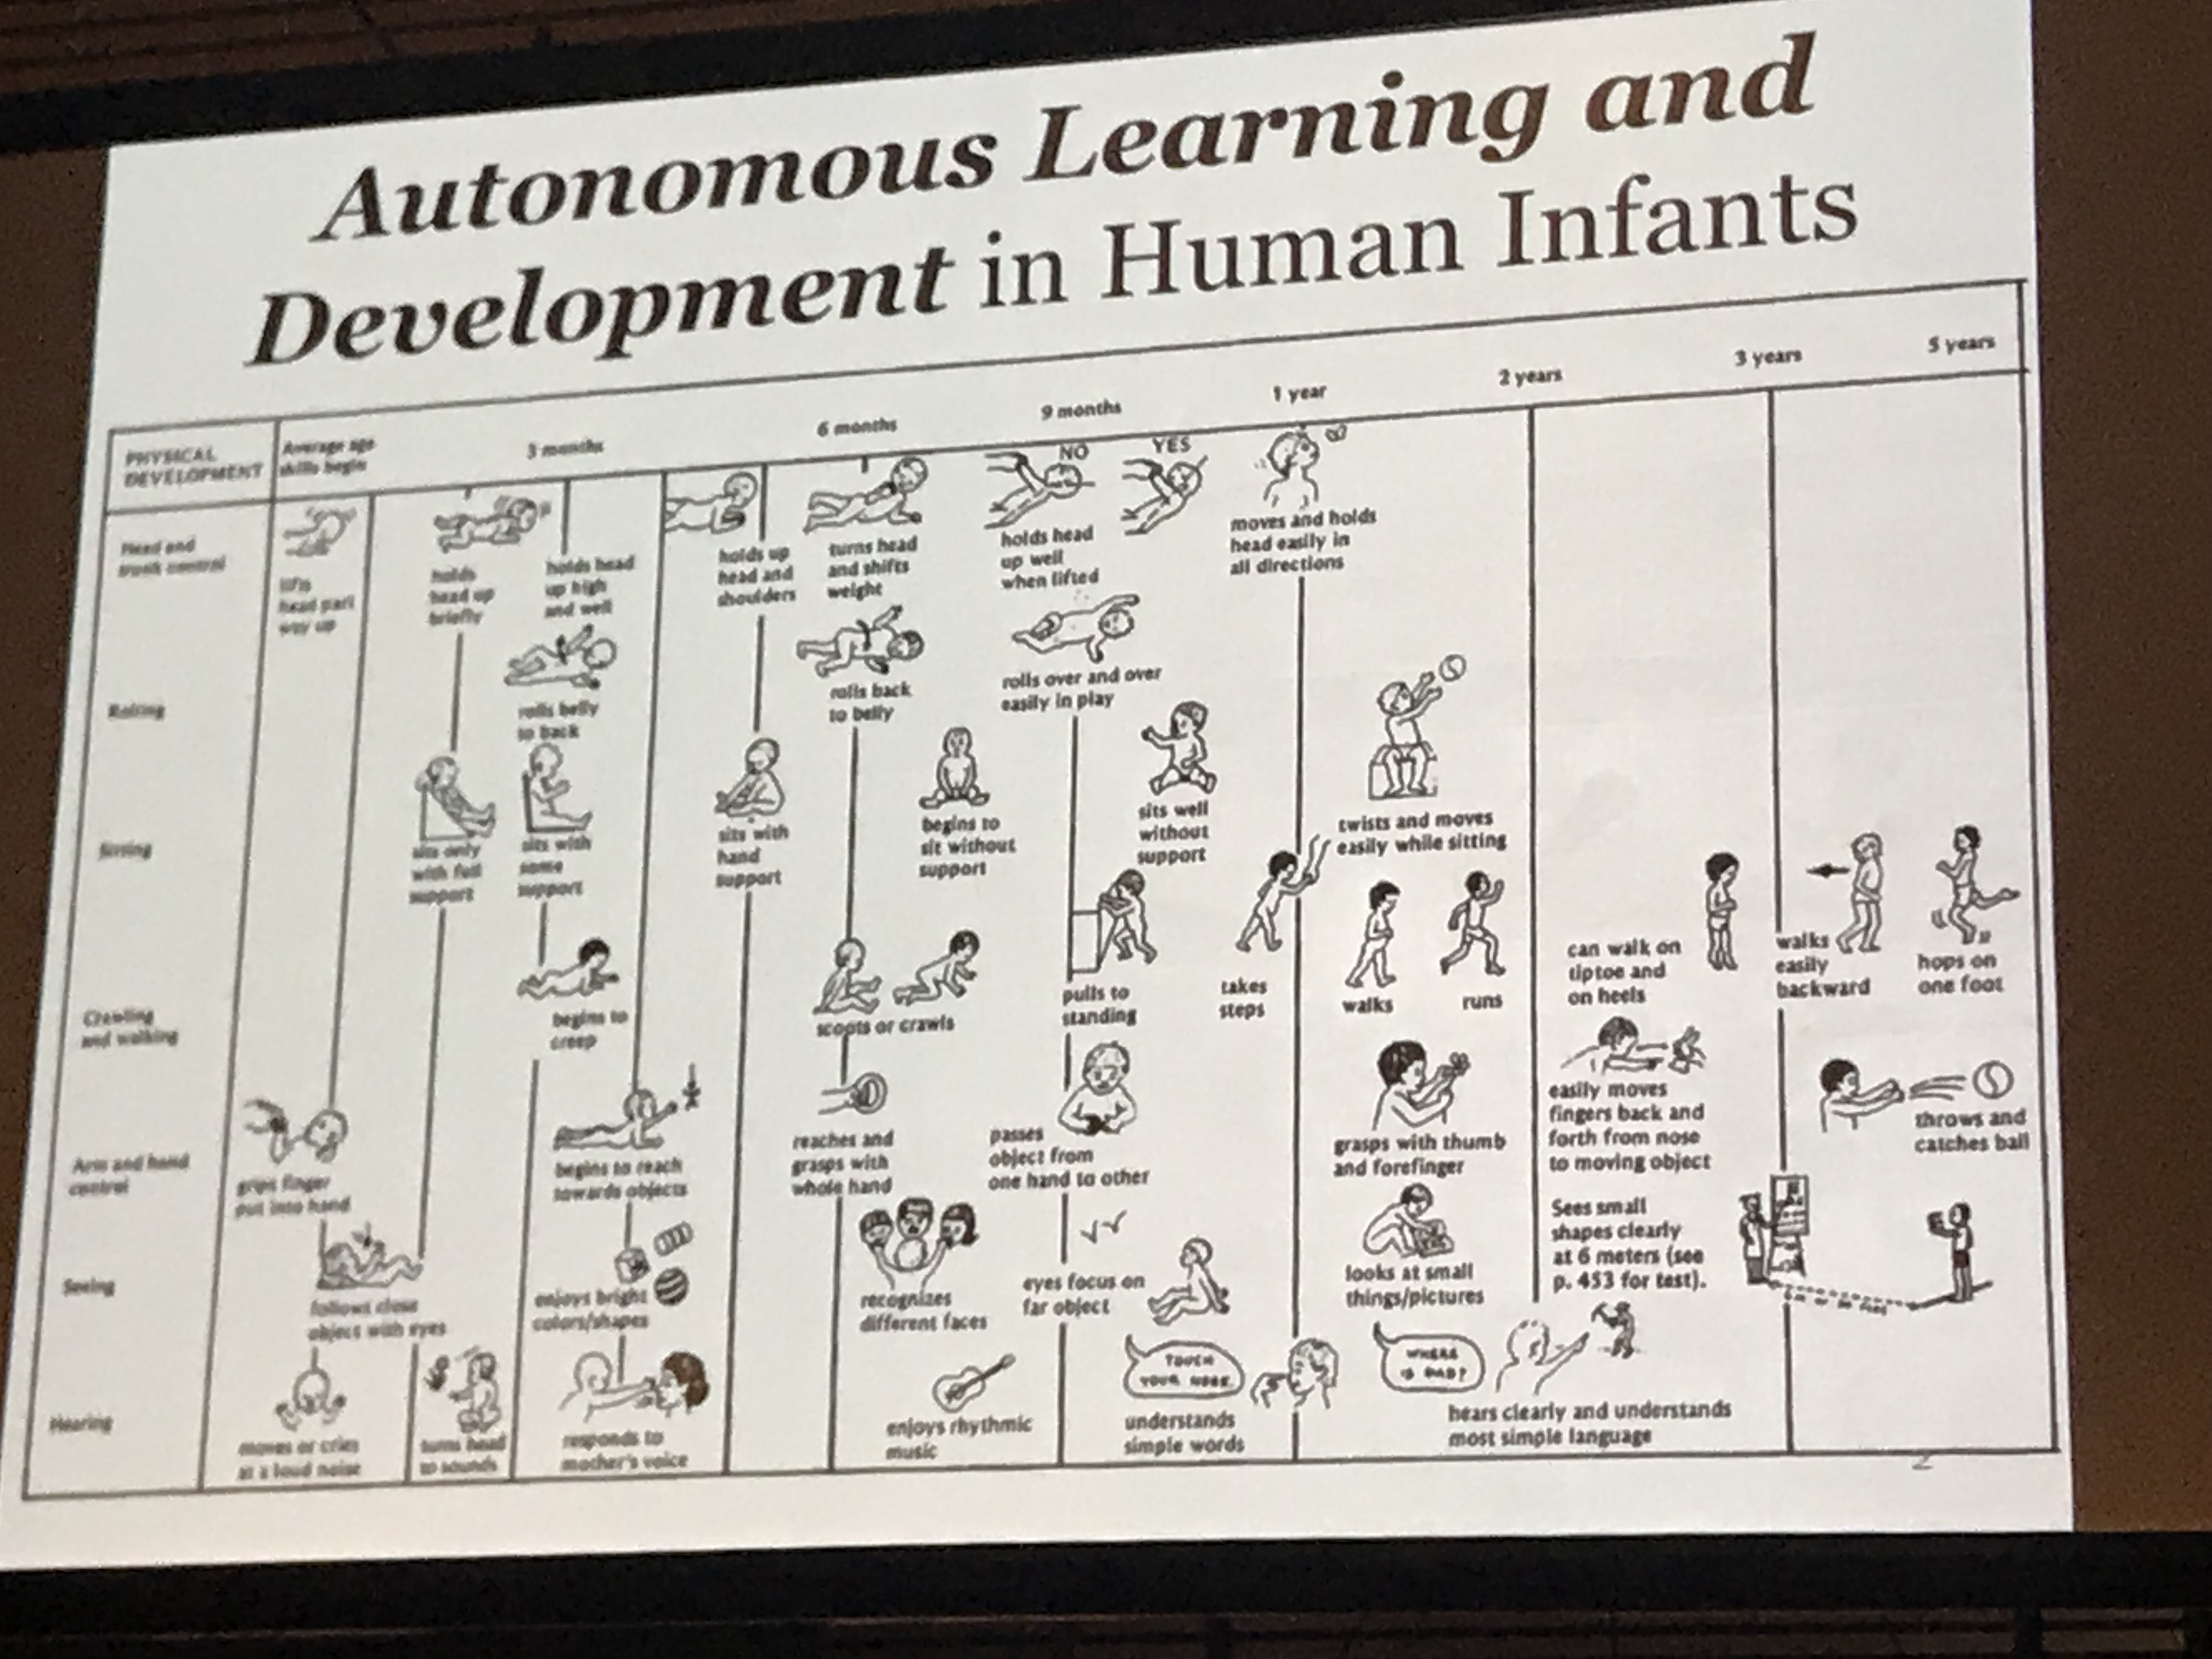
\includegraphics[width=0.4\textwidth]{images/child_learners.JPG}
    \caption{Learning and development in human infants.}
    \label{fig:child learners}
\end{figure}

Guiding Fields:
\begin{enumerate}
    \item {\it Cognitive Science:} Understanding human development and learning
    \item {\it Robotics:} new theory for lifelong and autonomous learning
    \item {\it Applications} in education technology.
\end{enumerate}


Example 1: study of {\it morphology}, body growth, and maturation in designing motor and perceptual primtives in a robot. \\

Example 2: consider language acquisition. Children learn new language very quickly. \\

Example 3: intrinsic motivation, play, and curiosity. \\

Q: How can we understand these practices, and harness them in AI tools, and build new educational tools around them? \\

\subsubsection{Intrinsic Motivation and Curiosity}

Consider {\it active exploration}: video of a baby playing with a variety of toys in a room over time (reminds me of the playroom domain from RL). \\

$\ra$ Similarly, give a baby a few toys, and a hollow cylinder suspended off the ground with a toy car inside of it. The baby over time tends to put the toy into the cylinder which knocks the car out of the tube (at which point the parent is very happy!). \\

$\ra$ But! When the car pops out of the tube, the baby also tends to pick up the car and put it back in the tube. \\

Other children experiment in very {\it different} ways; one kid picked up the block and hit the cylinder to make noises, and seemed very pleased by the noises. This was considered a ``failure" in the study, but was pretty sophisticated exploration! \\

{\bf Note:} Theories of intrinsic motivation, curiosity, and active learning drive to reduce uncertainty, experience novelty, surprise, or challenge. See~\citet{berlyne1960conflict} and~\citet{berlyne1978curiosity}. \\

{\bf Perspective:} The child is a sense making organism: explore to make good predictive models of the world and control it! \\

Q: Based on this perspective, what kind of modeling/algorithms are needed in order to explain these behaviors? \\

A: We use robotic playgrounds -- place robots in a playroom like environment, and encourage them to play to learn object models and affordances. Also place another robot in the playroom that gives ``feedback" (positive/negative reward) to play the role of a parent encouraging/discourgaing the baby.\\

Essential ingredients in these robots:
\begin{itemize}
    \item Dynamic movement primitives
    \item Object-based perceptual primitives (like infants, build on prior perceptual learning)
    \item Self supervised learning forward/inverse models with hindsight learning
    \item Curiositry-driven, self-motivated play and exploration.
\end{itemize}


\subsubsection{The Learning Progress Hypothesis}

Q: What is an {\it interesting} learning experiment for a robot/baby to conduct (to learn)? \\

Lots of answers in the literature: high predictability, high novelty, high uncertainty, knowledge gap, novelty, challenge, surprise, free energy, and so on. \\

{\bf This Work:} The Learning Progress Hypothesis~\cite{oudeyer2016intrinsic}:

\ddef{Learning Progress Hypothesis}{The ``interestingness" of an experiment is directly proportional to empirical learning progress (absolute value of derivative of the errors)}

$\ra$ Few assumptions on underlying learning machinery and on match between biases and real world. \\


{\bf Framework:} suppose we have some robots with motion primitives. Takes some sequence of actions to yield a trajectory:
\[
\tau = (s_t, a_t, s_{t+1}, \ldots).
\]
From this trajectory, the robot should learn, assuming some behavioral abstraction $\phi$:
\begin{enumerate}
    \item Forward model: $F_i : s, \theta \ra \phi_i$, with $\theta$ the parameters of the behavioral policy, $\pi_theta$.
    \item Inverse model: $I_i : s, \phi_i \ra \argmin_\theta ||\phi_i - F_i(s,\theta)||$
\end{enumerate}

Use these two models to measure ``competence progress" as a proxy of the empirical learning progress. \\

$\ra$ Example 1: hierarchical multi-armed bandits. Split a space into subregions, where an agent monitors the errors of each subregion. Use these errors to measure the learning progress over time. Then, in the bandit setting, can explore based on the ratio of these errors over time. \\

$\ra$ Example 2: explore omni-directional locomotion. Look at diversity (in terms of spread of states reached in some space) of outcomes by different exploration policies on a robot. Finding: curiosity-driven exploration is less-efficient than goal exploration.\\

Q: Why is curiosity driven exploration less efficient? \\

A: Forward model exploration (curiosity): knowing many ways to produce a few effects, inverse model exploration (goal): knowing a few ways to produce many effects. \\

Example: curiosity-driven discovery of tool use. Videos of a few robots playing with different tools (a robot with a cup learning to interact with a ball, a gripper robot learning to interact with a joystick). \\

$\ra$ Point: focus on playing with and manipulating objects in the world. The gripper robot learns to manipulate the joysticks, which moves the robot that can pickup the ball. Torso eventually learns to make a light, play a sound, and hide the ball in the cup. \\

Project: ``MUGL: exploring learned modular goal spaces"~\cite{laversanne2018curiosity}. Main idea is to extend these exploration techniques to high dimensional input (the robot examples above used a feature vector, not images). \\

$\ra$ MUGL can be used to discovery independently controllable features (learn to control a ball, and so on).

\subsubsection{Models of Child Development Data}

Experiment: modeling vocal development. Use exact same algorithms from before. \\

$\ra$ Goal: make experiments for the infant using the learning progress idea from before. \\

{\bf Finding:} Some self-organization of developmental structure in infants. First vocal track is learned (unarticulated sounds) and then learns articulated sounds. \\

$\ra$ Observe: regularities that tend to occur at the same time across different individuals, but some things change dramatically. Interactions between learning system and body morphology is stochastic, contingency in exploration, surprising that many things remain constant. \\

\begin{figure}[h!]
    \centering
    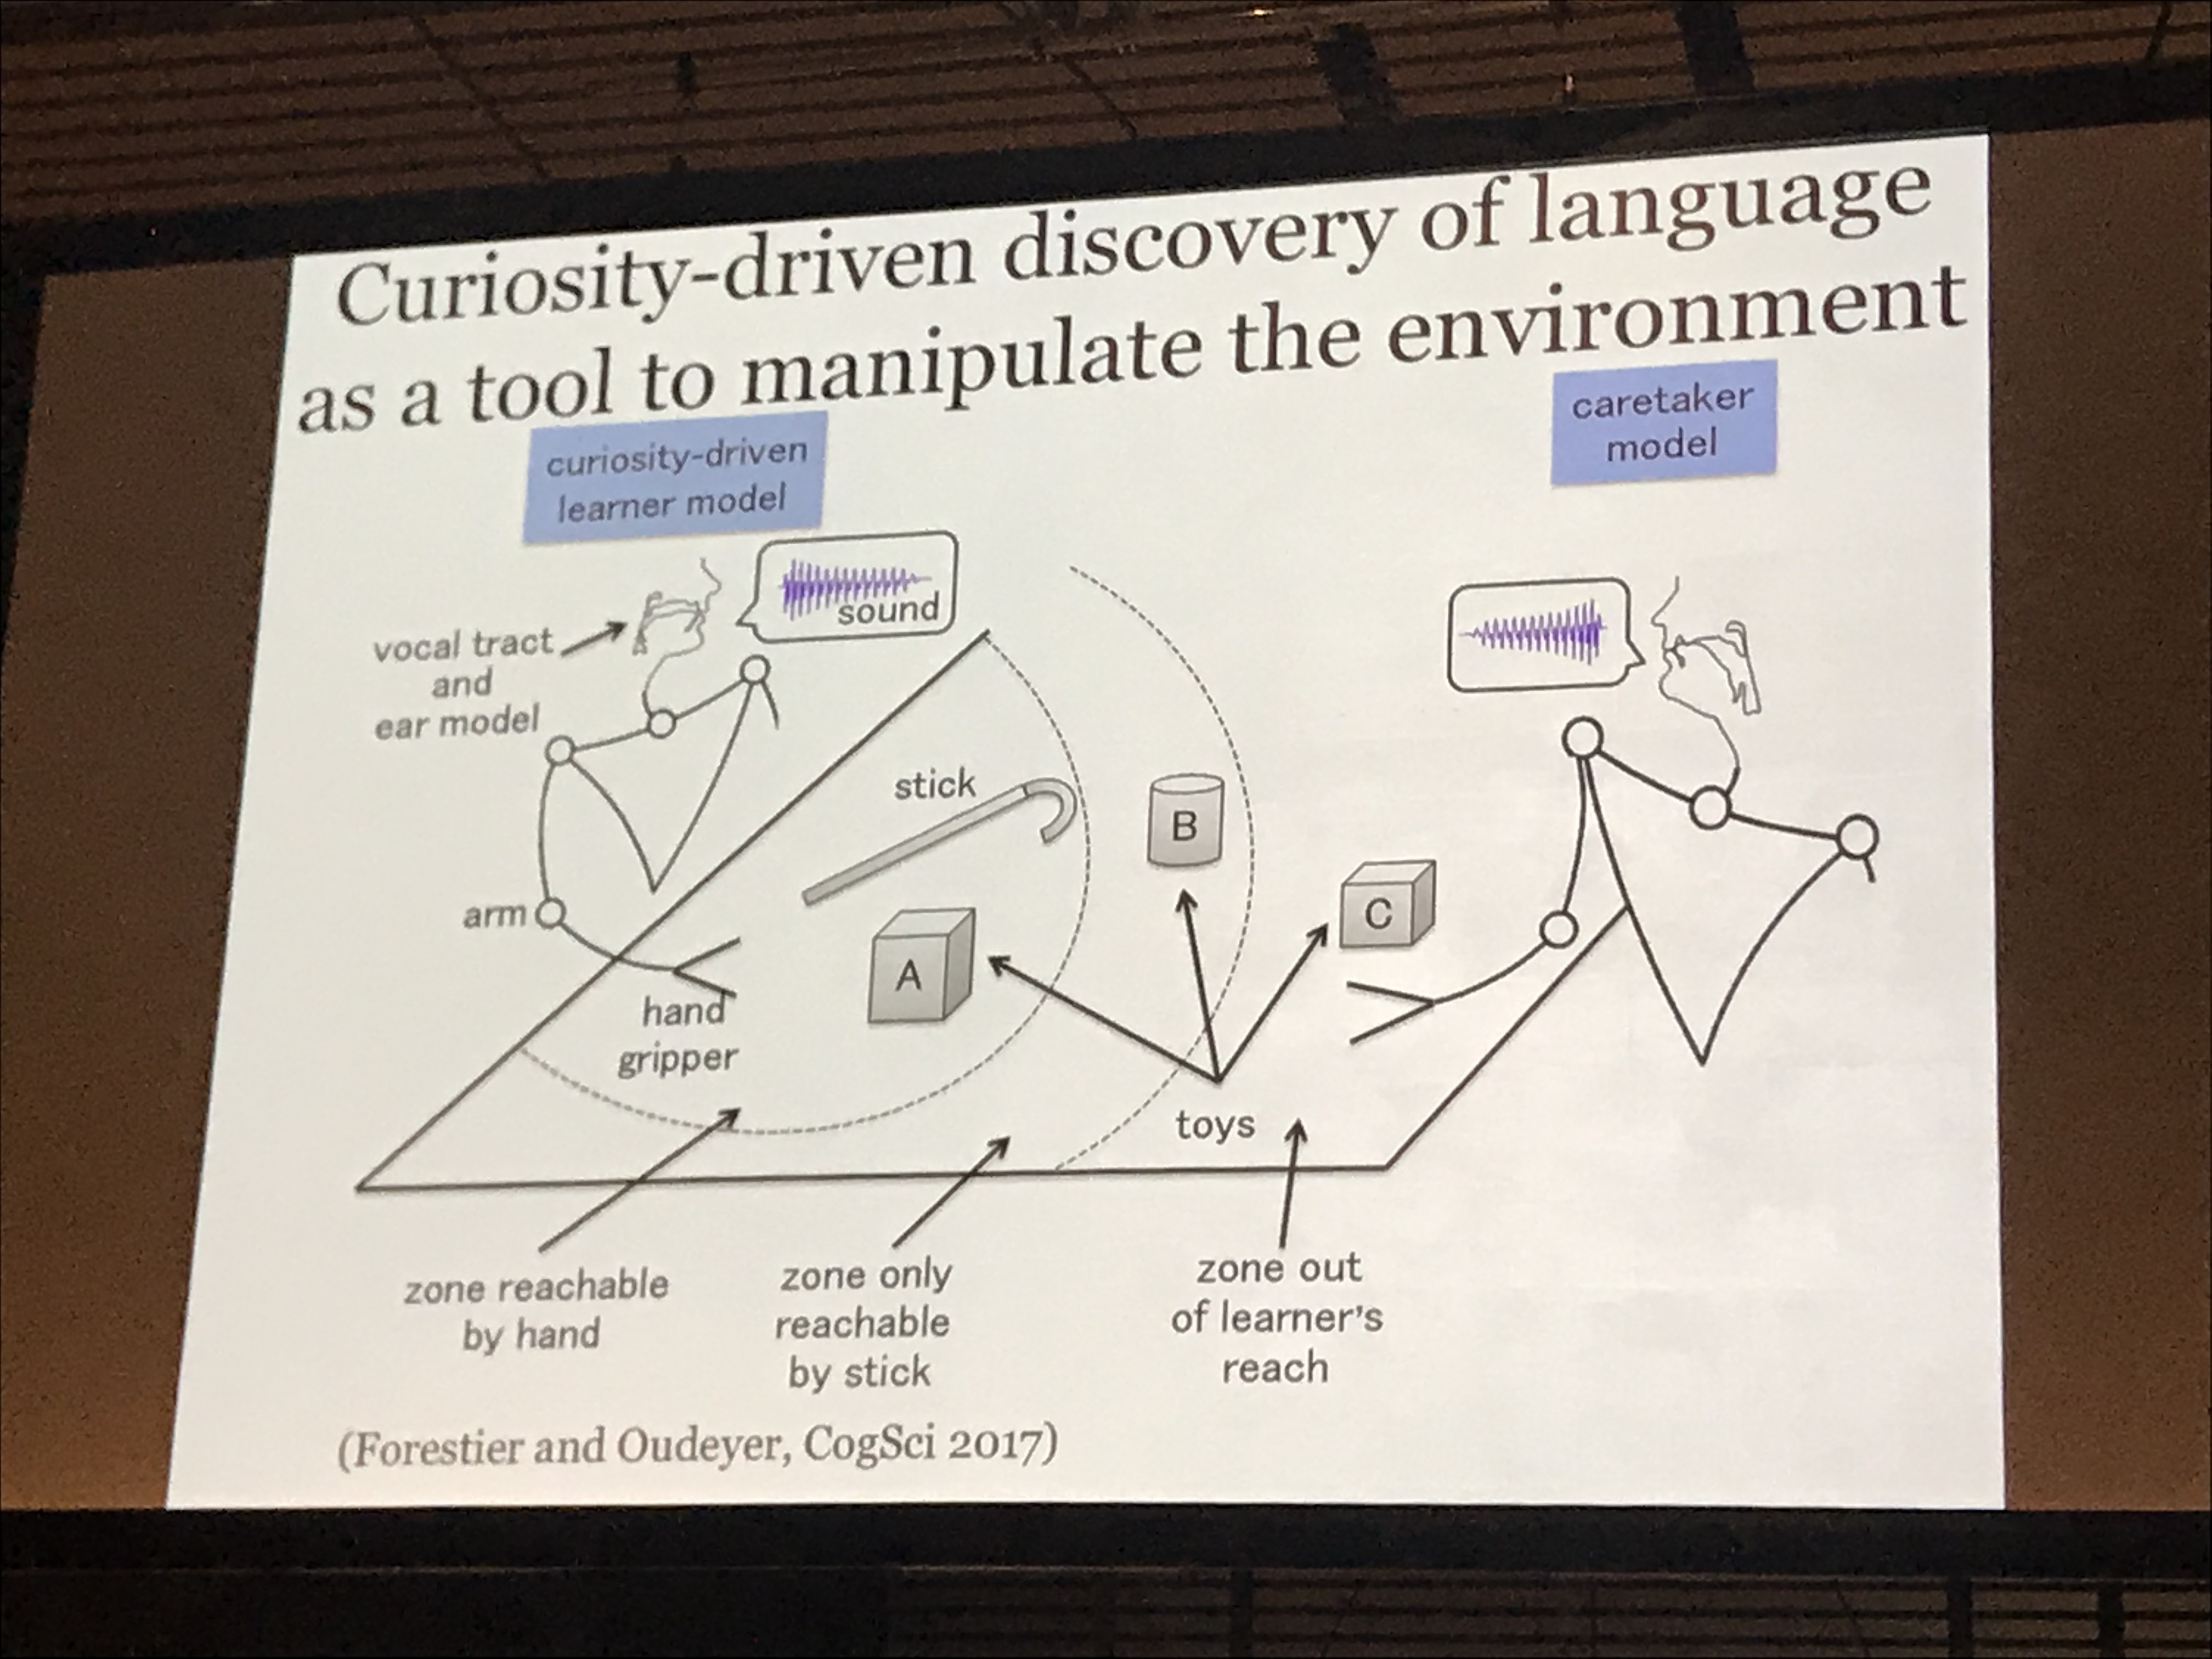
\includegraphics[width=0.4\textwidth]{images/curious.JPG}
    \caption{Curiosity-driven discovery of language}
    \label{fig:curiosity}
\end{figure}

The ``Ergo-Robots" (with Mikhail Gromov and David Lynch, I think?) \dnote{Lynch! :o}. Surreal video of robots learning to speak and interact with their environment and companions, see a sample video here: \url{https://www.youtube.com/watch?v=J0gM5i091JQ}. Robots learn to use language in a meaningful way through exploration. \\

$\ra$ Use similar ideas to come up with a realistic models of learning to use a vocal track. See: {\it Self-Organization in the Evolution of Speech}~\cite{oudeyer2006self}. \\

{\bf Finding:} The distributions of vowels we find in the world languages matches those of the systems that emerge in these curiosity-driven learning systems. This might explain some regularities of language structure. \\




Q: How is spontaneous exploration structured during free play? \\

A: Experiment! Let subjects play a bunch of games/tasks, with no guidelines. Just do whatever you want (play games like guitar hero, free to pick any level/song). \\

$\ra$ People tend to focus on levels of intermediate complexity; exploration follows a controlled growth in complexity, actively controlled by individuals' predictive models. 


\subsubsection{Applications in Educational Technologies}


{\bf Goal:} Develop technologies for fostering efficient learning and intrinsic motivation. \\

$\ra$ Project: KidLearn -- allows personalization of intelligent tutoring systems, based on experiments with $>$ 1000 children in 30+ schools. \\

Principle: graph (usually a DAG) defines difficulty of task/exercise type. This allows the system to sample exercises in some sequence (but still give the kids some choice among nodes in the graph). \\

Main study:
\begin{itemize}
    \item Examine learning impact based on these interventions.
    \item Compare to typical pedagogical expert (vs. their system).
    \item Find that students tend to achieve higher success rate with certain variations of the algorithm.
\end{itemize}

{\bf Takeaways:} Fundamental role of spontenous developmental exploration, can be harnessed to develop human-like robots and empower the learning process.

\subsection{Contributed Talks}
Next up some contributed talks.

\subsubsection{Devon Hjelm on Deep InfoMax~\cite{hjelm2018learning}}

{\bf Broad Goal:} Learn unsupervised image representations. \\

Example: video of a dog catching a snowball. What annotations make sense? (``Cute dog!", ``Good boy!"). \\

$\ra$ Not clear these are the right/useful annotations. \\

{\bf Point:} Don't always want supervised learning of representations. Annotations rarely tell the whole story, real world doesn't come with labels, and really want to find the underlying structure (annotations might not enhance this part). \\

Preliminaries:
\begin{itemize}
    \item Encoder: $E_\psi : \mc{X} \ra Y$, with $Y$ a representation.
    
    \item Mutul info; $I(X;Y) = D_{KL}(P(X,Y) \mid \mid P(x) p(y)$
\end{itemize}

$\ra$ Introduce amutual information estimator: encode an image into a representation. Take pairs of representations from images that aren't associated with each other, and treat these as {\it negative} samples,. \\

{\bf Approach:} 
\begin{enumerate}
    \item Encode input $X$ input $Y$ via $E_\psi$.
    \item Use output to estimate $\hat{I}(X;Y)$, and maximize this estimate.
    \item Just doing this alone isn't quite enough.
    
    {\it Intuition:} you might not pick up on the relevant locations of an image. Consider a picture of a cat, the background isn't as crucial as the information in the front.
    
    \item So: instead of maximizing the mutual info globally, instead maximize it {\it locally}. Perform this estimation/maximization across all locations simultaneously. See Figure~\ref{fig:cat}
    \item This yields local feature vectors for different regions of the image, which can then be stitched together into a global feature vector.
\end{enumerate}

\begin{figure}
    \centering
    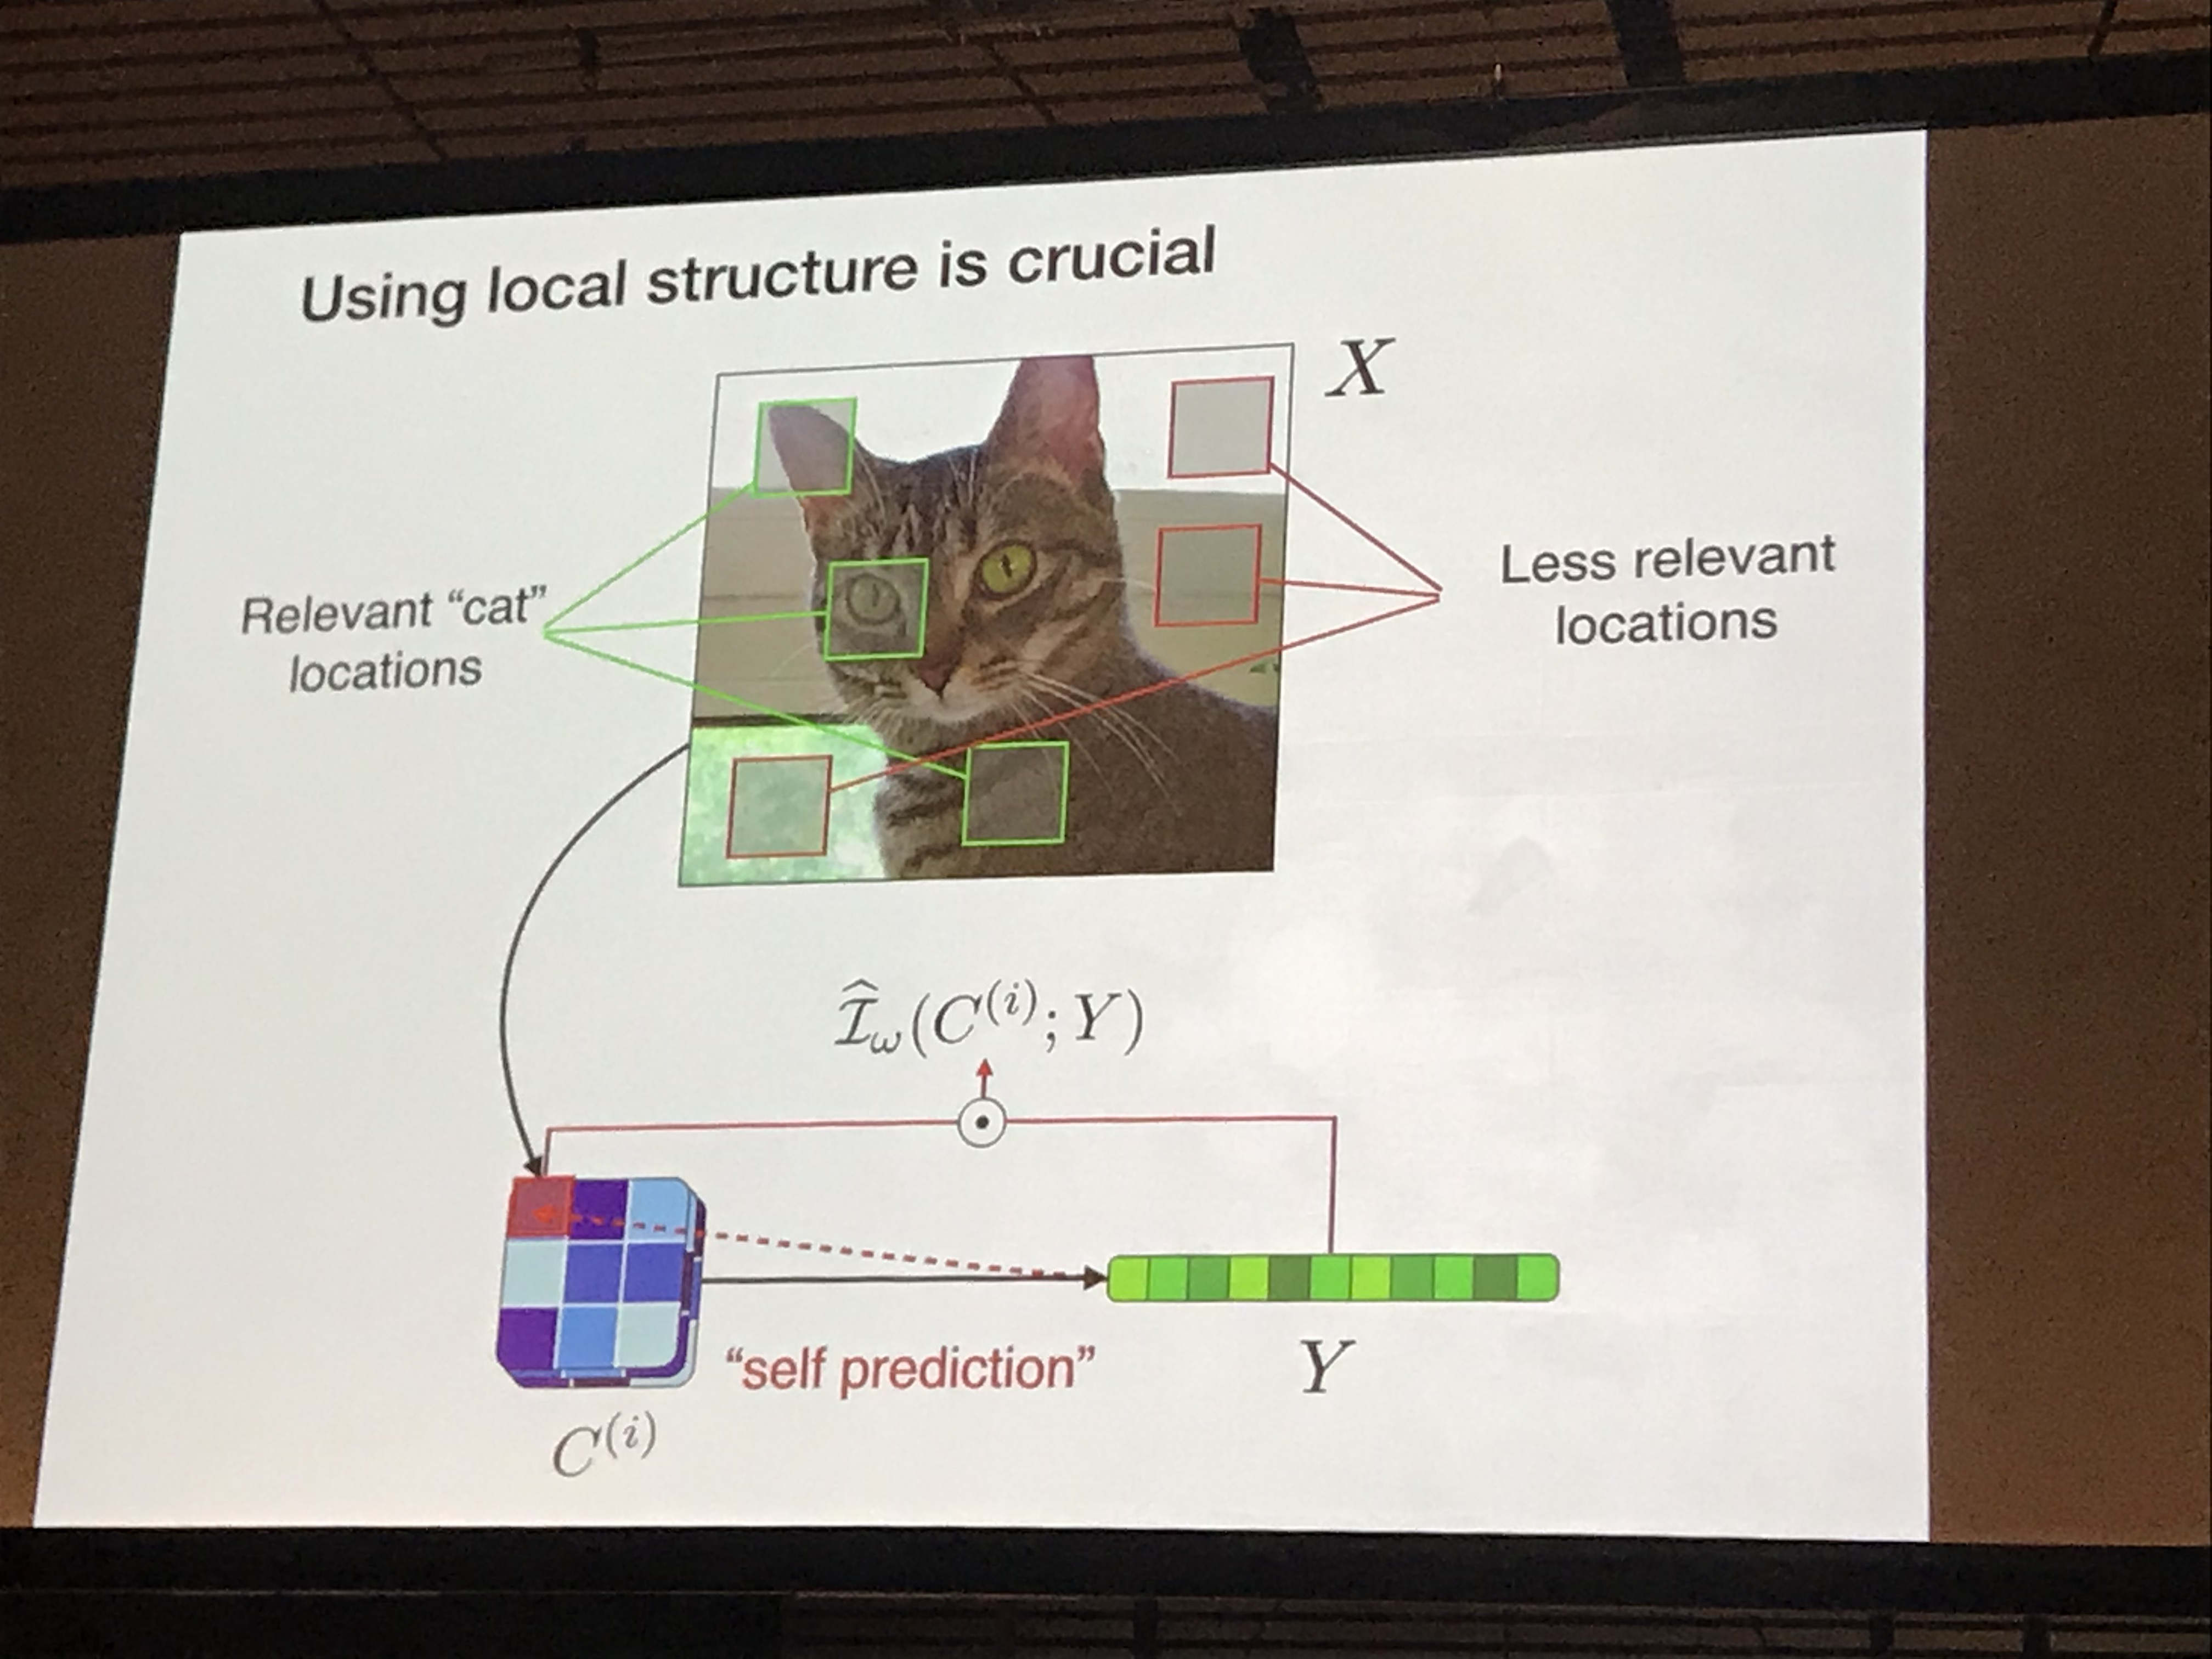
\includegraphics[width=0.4\textwidth]{images/cat.JPG}
    \caption{Extracing local feature maps via local mutual info estimation and maximization}
    \label{fig:cat}
\end{figure}

Evaluation: depends heavily on downstream task. Can measure mutual info, down stream performance on classification/regression tasks, and so on. \\

$\ra$ Deep Info Max performs very well when the learned representation is used in downstream tasks like classification. \\

Other tasks investigated: prior matching, coordinate prediction, relative coordinate prediction \\

\dnote{Off to more meetings.}

\subsection{Keynote: Zeynep Tufekci on Dangers if ML Works}

Grew up wanting to be a physicist! But: eventually, many physicist encounter the {\it nuclear} problem: massive ethical issues facing the advancement of a scientific field. \\

$\ra$ At CERN recently: giant projects! 700 people on the Higgs Boson paper. They were concerned about how to divide up the Nobel prize, meanwhile in CS we're worrying about the impact our tools have on society, security, labor, climate, social infrastructure, and beyond. So: lots of ethical issues in CS, too! \\

Back in Turkey: no internet, limited access to culture/TV from the outside world (grew up watching little house in the prairie). But, got internet connection through working at IBM. \\

$\ra$ Wonderful to have unimpeded access to lots of information and connections to people! Lots of optimism about the power for this tool to do good in the world \\


{\bf This Talk:} big dangers that we're sleepwalking into. Going to end up in a scary and unhappy place, we will end up having built and contributed to part of it. \\
\begin{itemize}
    \item Seven years ago: the ``cat" paper, that learned to recognize cats on YouTube. Was hard to even imagine the current state of the field back in 2012.
    \item What we need to worry about: what if it works? What are we really introducing into the world?
\end{itemize}


{\bf Themes:}
\begin{enumerate}
    \item You are part of this world, and your tools will be too.
    \item These tools won't be used the way you think they will be.
    \item Alternative paths are possible.
\end{enumerate}

\subsubsection{Examples Of Ways Things Can Go Wrong}

Example 1: social movements in the public sphere. Specifically, the Facebook news feed:
\begin{itemize}
    \item Optimized to keep people engaged on the website
    \item Recall: Ferguson, MZ, shooting of an african american teen by a police officer. Similarly: in a McDonalds, some customers were thrown into a van without any chance to say anything (by some police officers).
    
    $\ra$ Huge discussions about these events on Twitter, but {\it not} Facebook. 
    
    \item Point: Friends {\it were} talking about it, but these issues weren't ``engagement friendly" for Facebook (it was trying to populate news feed with things that would be liked/shared).
    
    $\ra$ At the time, the ALS ice bucket challenge was going as well. Very likeable/shareworthy, so that dominated most Facebook news feed.
    
    $\ra$ Chilling moment: icebucket challenge dominated the media/facebook as a result.
\end{itemize}

Difference for social movements isn't whether you hold a protest. The thing the movements manage to do to be most effective is get attention. \\

$\ra$ But our algorithms are optimized to keep people engaged, so it tends to not spread certain kinds of information. A new form of censorship. \\

{\bf Classic finding:} People that tend to be into one conspiracy theory tend to be into others (from social science). \\

$\ra$ Instagram would recommend similar conspiracy theories, not because designers recommend them, but just because the algorithm learned this social science fact (someone likes a ``faked moon landing" post will also be presented with tons of other conspiracy theories). \\

in 2016: these phenomena were {\it widespread}. Watching one certain kind of video would immediately bias future videos (if you watch a jogging video, it then leads you to hardcore marathon training, if you watch a vegetarian video, it then leads you to vegan videos). \\

{\bf Point:} YouTube algorithms tends to {\it lead individuals down more polarizing and extreme routes}. Not by hand-design, but it does it {\it to increase engagement}. \\

$\ra$ Hate speech, extreme views, and so on, are very ``shareworthy" and capable of improving engagement.

\subsubsection{ML and its Challenges}

Some core challenges of implementing ML systems in the world:
\begin{enumerate}
    \item Bias
    \item Interpretability
    \item Potency-at-scale Restructuring power
    \item Surveillance and Privacy
    \item Transition and Upheaval
\end{enumerate}

Example: suppose you're hiring, and suppose you use ML to hire. \\

(rhetorical) Q: We have methods for predicting depression rates; what if your ML system in using this information for hiring outcomes? \\

Problem: You won't even know that your system is using this information! \\

Similar problem: can use a ``mirror population" system (identify similar groups) to target individuals that are fear-prone with well designed ads to encourage voting for authoritarians? (again coming from findings in social science). \\

$\ra$ The way these systems are built {\it incentivizes} surveillance, since data about individuals/groups is always important. Data {\it will} get out, and will be used. \\

{\bf Path Forward:} build things that can do what we want to do, but not let it control us and be used on things we dont want it to be. \\

**We are in a very particular historic moment: all the companies here are trying to recruit you. If these companies that are trying to recruit you, but can't get you to do the things they want you to do, but you {\it insist} on using privacy-preserving methods. \\

{\bf Takeaway:} Lots of good the talent in this room can do. \\

Some thoughts:
\begin{enumerate}
    \item Google gave away money for ML projects. One of them was on detecting societal ideation, someone at risk, and do intervention.
    
    Seems like a great 
    
    \item What will happen: university will expel kids with mental health issues. They don't want that happening in their dorms.
    
    \item Look at the database of people killed by police officers. Many people are in a mental health crisis.
    
    $\ra$ Suicide detection program can be used in a very bad way (like laws that prevent at risk individuals from basic needs/goods).
    
    \item But! Imagine a privacy preserving system designed to help individuals instead.

\end{enumerate}

First earth day: pictures were blurry because of smog. Now that's not the case! So, a final note: genuinely consider unionizing. \\

Union: you get a huge number of legal protections. You get some freedom of speech. Organize your own industry ML group. \\

No one here is trying to explicitly go down this dark path. So many good people in this community! But the business model plus the world leads us to the wrong kinds of systems.

Final thoughts:
\begin{enumerate}
    \item Organize
    \item Build alternatives
    \item Insist on having a voice
\end{enumerate}

*What we want, when someone wants to have a phone/app, we're just doing a bad job of what China is doing (in terms of monitoring/surveilance) for the purpose of selling more stuff. \\

$\ra$ We need a real alternative. We need the conveniences and empowerment, we need an option that repsects us, that gives us early warning and intervention but not at the expensve of subjecting us to mass surveilance. \\

{\bf Final Example:} Before Diffie-Helman (public key crypto), we didn't have a way of sending a message without exchanging secret keys. 
\begin{itemize}
    \item They thought this was a terrible problem. Needed to give people a way to communicate and exchange info without having to exchange keys beforehand.
    
    \item All of public key crytography comes from that. Really important and invidual-empowering tool that has dramatically reshaped the state of the world.
    
    \item So: stock options are cool, but we should be thinking about developing tools like this for the next generation of technology.
\end{itemize}





% ---------------
% -- Wednesday --
% ---------------
\newpage
\section{Thursday May 9th: Main Conference}
Last day! I'm flying out this afternoon so I will only make a few sessions today.


\subsection{Contributed Talks}

Now some contributed talks.

\subsubsection{Felix Wiu on Pay Less Attention with Sequence Models~\cite{wu2019pay}}

{\bf Observation:} Sequence models are almost everywhere in NLP (have become the CNN$\leftrightarrow$ vision). \\

This work:
\begin{enumerate}
    \item Q1: Is self attention needed for good performance?
    \item Q2: Can we do well on a range of NLP tasks with limited context?
\end{enumerate}

Different models perform very differently on Neural machine Translation (Transformer achieve BLEU of 28, SliceNet of 25, phrase-based of 22). \\

$\ra$ Large performance gap of self-attention and convolutional models. \\

Background: three ways to encode a sequence
\begin{itemize}
    \item RNN: recurrent neural net.
     can.
    $h_t = f(x-t, h_{t-1})$, with $x_i$ the input at time $i$, $h_i$ the hidden state at time $i$.
    
    \item CNN: convolutional neural net.
    
    $h_t = f(x_{t-k}, \ldots, x_{t+k})$ $\ra$ look at a limited window.
    
    \item Self-attention models: Compute pairwise similarity between words and aggregate them.
    
    $h_t = \sum_{i,j} a_{i,j}$.
\end{itemize}

Some pros and cons of each! RNNs can't be parallelized, while CNNs and self-attention, time complexity is higher for self-attention, and so on (see Figure~\ref{cnn_rnn} for full comparisons). \\

\begin{figure}[h!]
    \centering
    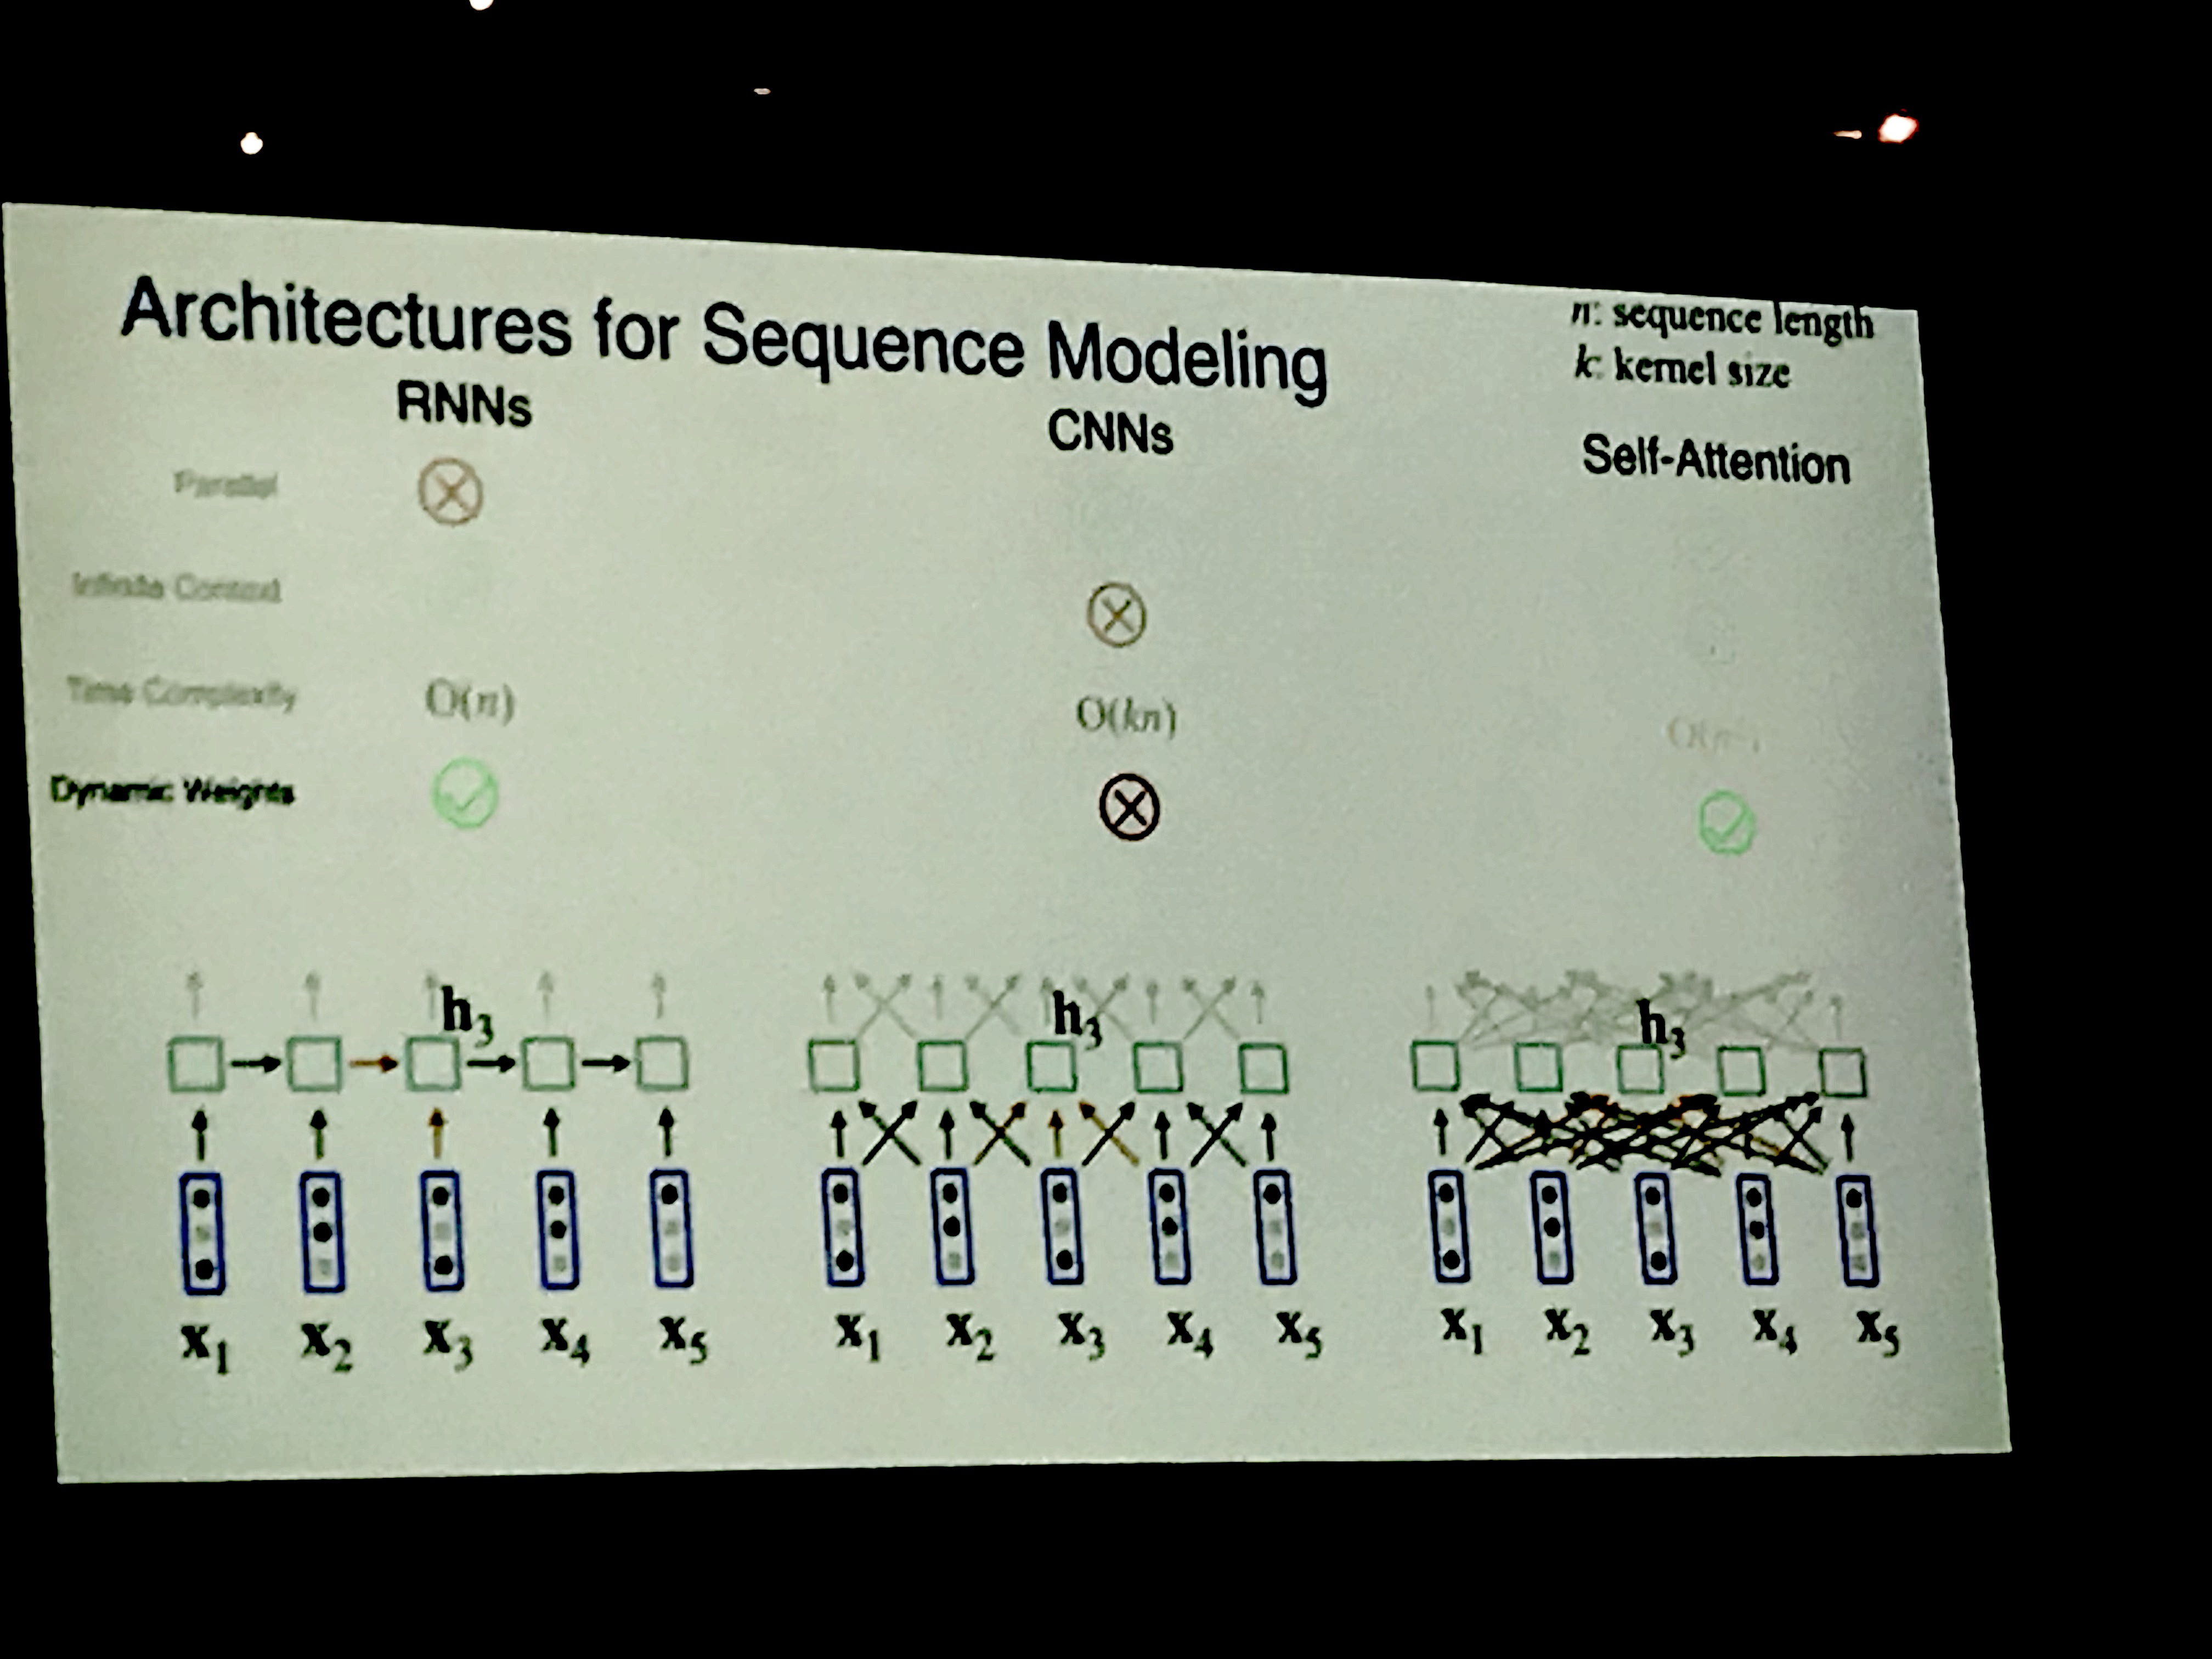
\includegraphics[width=0.4\textwidth]{images/cnn_rnn-2.JPG}
    \caption{Pros and Cons of CNNs, RNNs, and self-attention for sequence modeling.}
    \label{fig:cnn_rnn}
\end{figure}

{\bf Approach:} {\it dynamic} convolution that addresses the main disadvantage of CNNs (lack of dynamic weighting). \\

But, some challenges to dynamic convolution: too many parameters to optimize! \\

$\ra$ Response: turn to lightweight convolution, which reduces the number of parameters. \\

{\bf Experiments:} Explore the trade-off made between {\it inference speed} measured by sentences per second) vs. {\it BLEU score}, which is a way to measure the quality of output translations. \\

$\ra$ Main finding: dynamic convolution achieves same BLEU score as self-attention, but with a 20\% speed up in inference time. \\

Conclusion:
\begin{enumerate}
    \item Local information is sufficient for several NLP tasks.
    \item Introduced dynamic convolution: context-specific kernels.
    \item Lightweight convolution: fewer convolution weights still work well.
\end{enumerate}


\subsubsection{Jiyauan Mao on Neural-Symbolic Context Learner~\cite{mao2019neuro}}

{\bf Focus:} Visual concept reasoning. \\

$\ra$ Given an input image (of some objects), people can quickly recognize the objects, texture, surface, and so on. \\

Visual Question Answering: given an image and a question ``What's the shape of the red object?", output an answer to the question. \\

$\ra$ Also, may want to do image captioning: ``there is a green cube behind a red sphere", or instance retrieval (a bounding box on a particular object). \\

{\bf Prior Approaches:} End-to-end approaches for solving these three problems. Two things to learn: 1) concepts (colors, shapes), and 2) reasoning (counts). \\

$\ra$ Downside to end-to-end: concept learning and reasoning are entangled. Not obvious how to transfer. \\

{\bf This Approach:} Incorporate concepts in visual reasoning. Prior methods rely on excpliti concept annotation. \\

The idea:
\begin{itemize}
    \item Joint learning of concepts and {\it semantic parsing}.
    \item Given a scene parser, and a semantic parser, learn a program that understands the concepts while parsing both objects.
\end{itemize}

Example: given an image of a red sphere and green cube, first perform object detection/feature extraction to get a representation. At the same time, do semantic parsing on the text, to output a parse program that predicts the output of the question. The full overview is given in Figure~\ref{fig:cube}

\begin{figure}[h!]
    \centering
    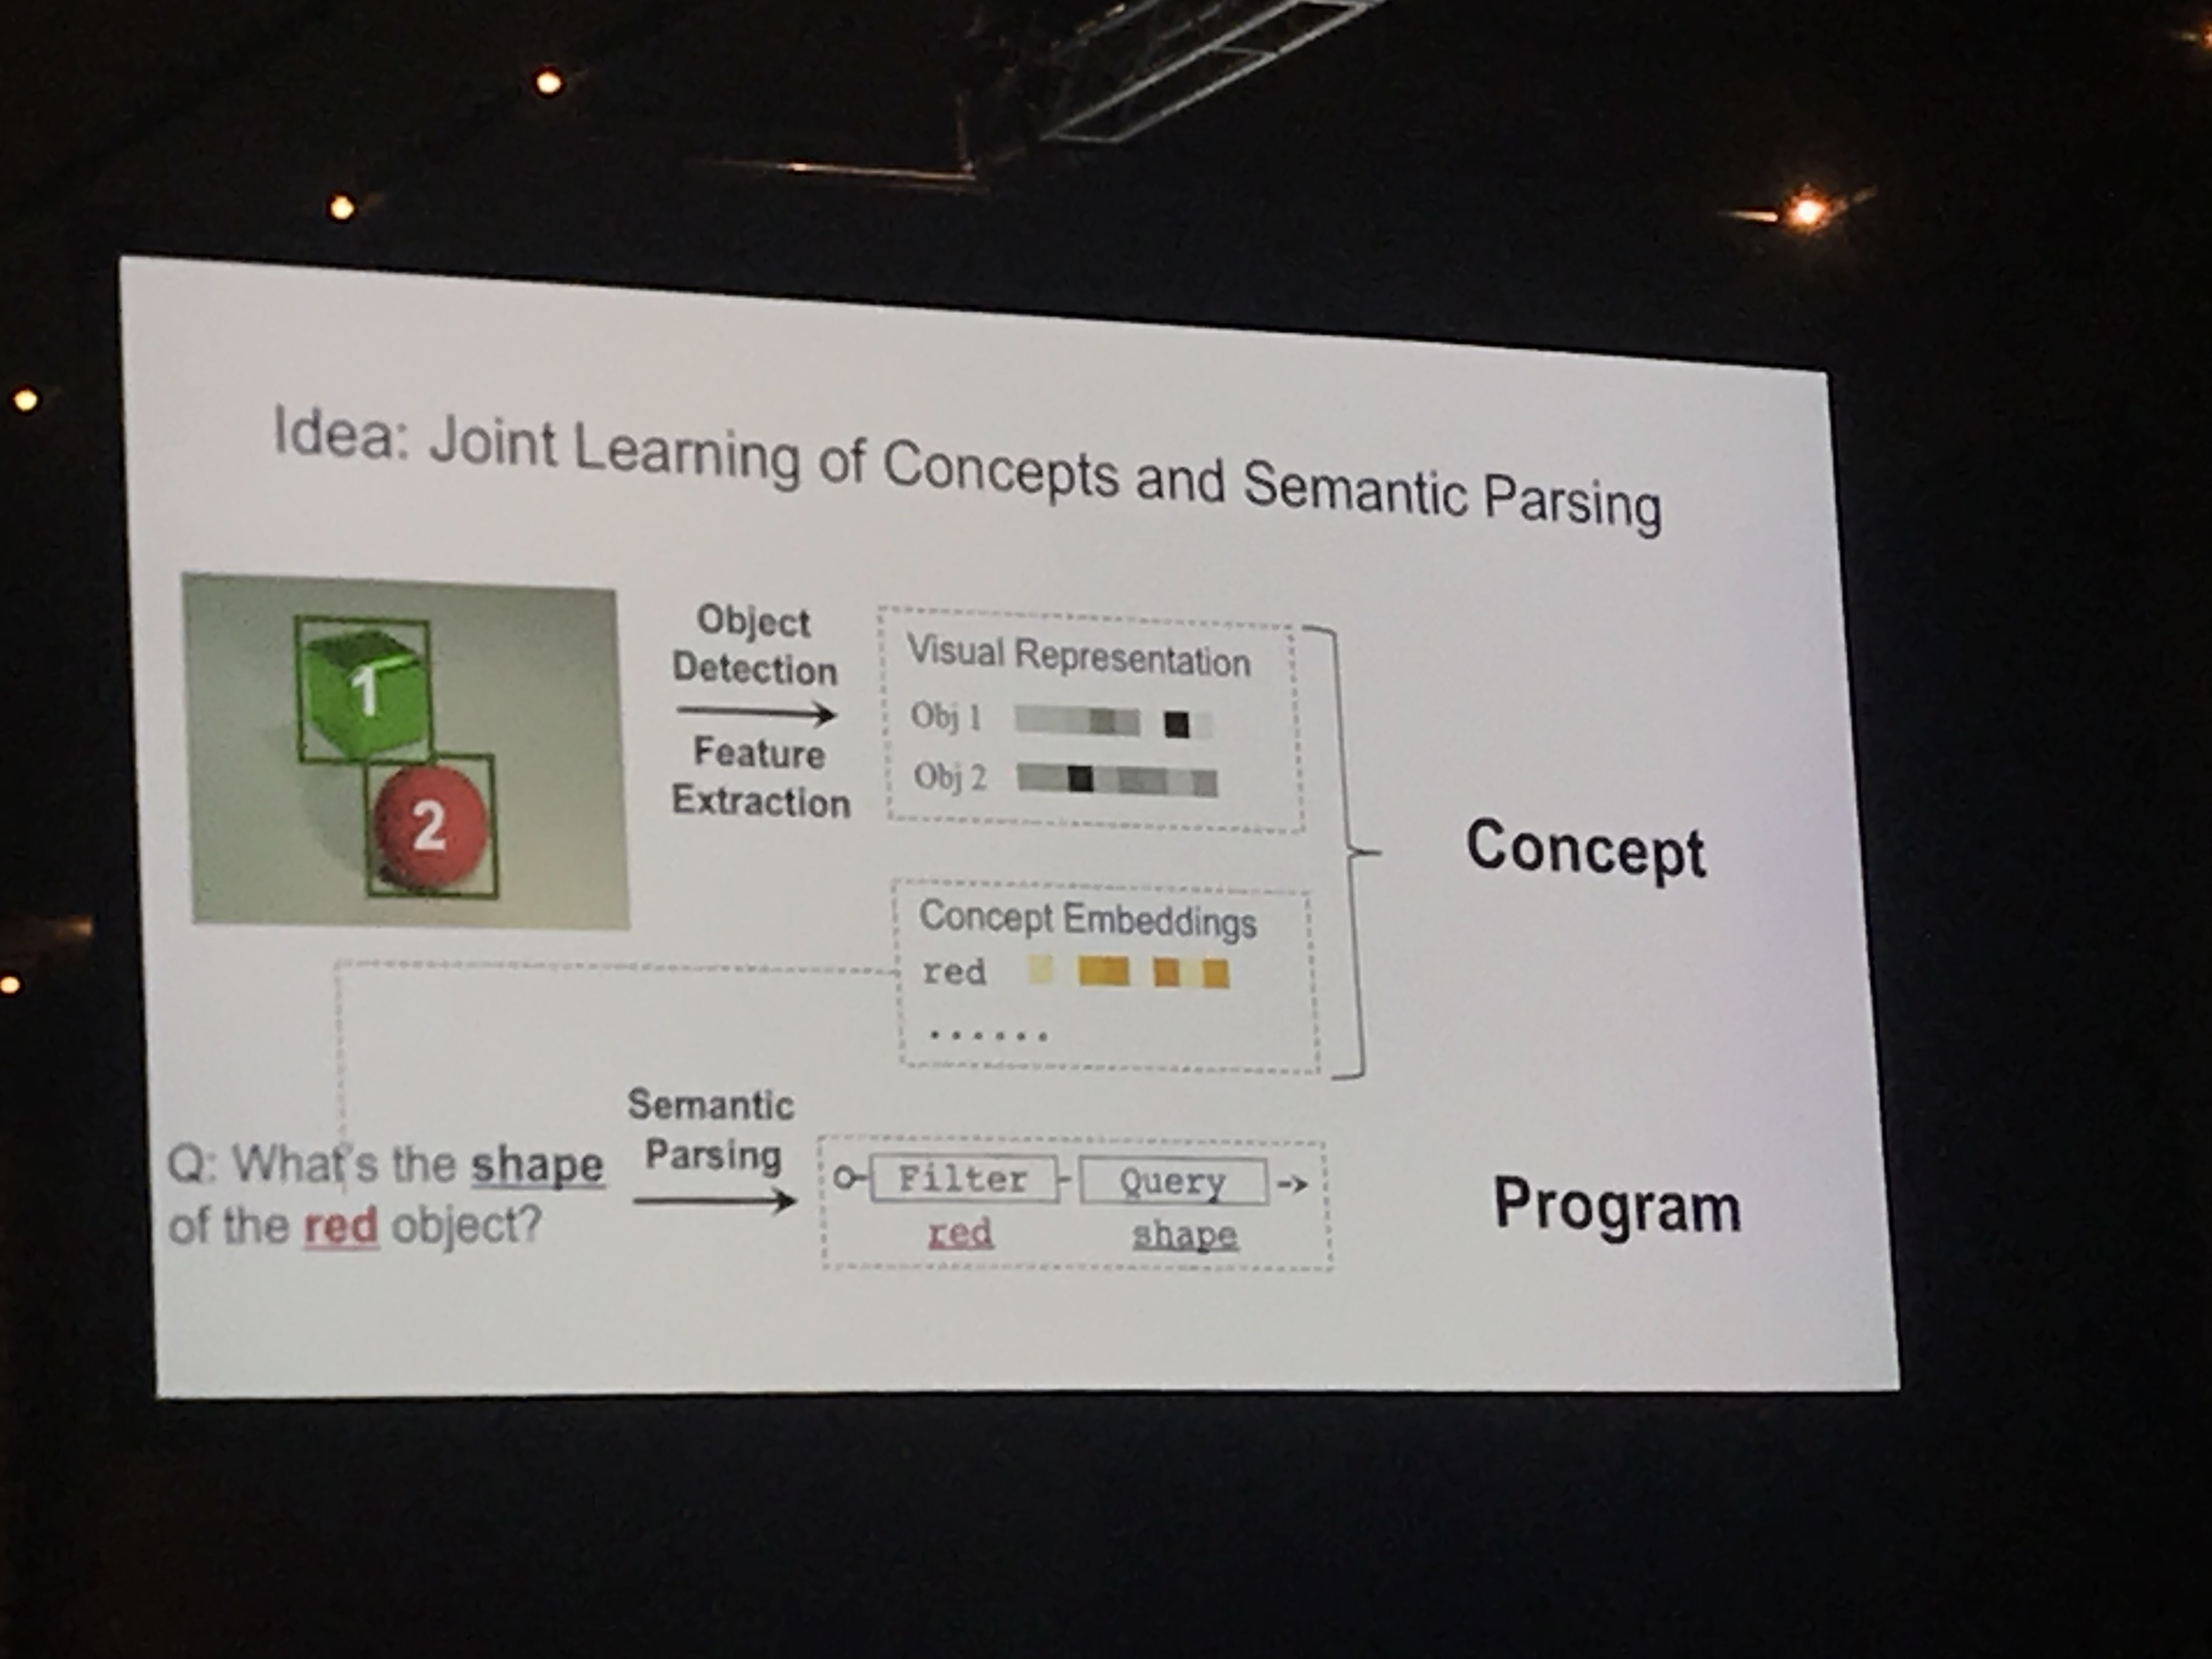
\includegraphics[width=0.4\textwidth]{images/cube.JPG}
    \caption{Overview of the approach for joint semantic and scene parsing.}
    \label{fig:cube}
\end{figure}

Two main methods:
\begin{itemize}
    \item Learn a program for understanding concepts
    \item Learn a concepts that can help facilitate parsing new sentences
\end{itemize}

{\bf Experiments:} This approach yields several advantages
\begin{itemize}
    \item State of the art performance on the "CLEVR" data set for visual question answering.
    \item Extensions to natural images and natural sentences as in the VQS dataset: ``what color is the fire hydrant?" given a natural seeming image of a fire hydrant (correctly guesses ``yellow").
    \item Model also supports composition of low level concepts into high level concepts, and bounding box detection.
\end{itemize}

{\bf Limitations and Future Directions:}
\begin{itemize}
    \item Consider example of a person with an umbrella hat on, and the question ``what purpose does the thing on this person's head serve"? proves extremely challenging!
    \item Recognition of in-the-wild images and beyond (like goals).
    \item Interpretation of noisy natural language
    \item Concept learning in a more sample efficient way.
\end{itemize}

Conclusions:
\begin{itemize}
    \item New model: NSCL learns visual concepts from language with no annotation
    \item Advantages of new model:  high accuracy and data efficiency, transfer concepts to other tasks.
    \item Principles: explicit visual grounding of concepts with neuro-symbolic reasoning.
\end{itemize}

\subsubsection{Xiang Li on Smoothing Geometry of Box Embeddings~\cite{li2018smoothing}}

{\bf Point:} Learning representations is crucial in NLP! These representations are usually vectors like word2vec or BERT. \\

$\ra$ These vectors define semantic similarity in space (closer together words have similar meaning/use). \\

But, consider: Rabbit/mammal. They're close to each other in space, but don't capture the full complexity of their relationship rabbit $\subset$ mammal). \\

$\ra$ One idea: Gaussian representation of classes like ``mammal". Advantages: 1) region, 2) asymmetry, 3) disjointness; but, one downside: not closed under intersection. Recent work extends this to a probabilistic model that gives up disjointness to achieve closure under intersection. \\

{\bf Their Approach:} An extension of these probabilistic models using a {\it box representation} to account for joint concepts, thereby achieving all four of the desired properties (region, asymmetry, etc.). Box representation seen in Figure~\ref{fig:box}. \\

\begin{figure}[h!]
    \centering
    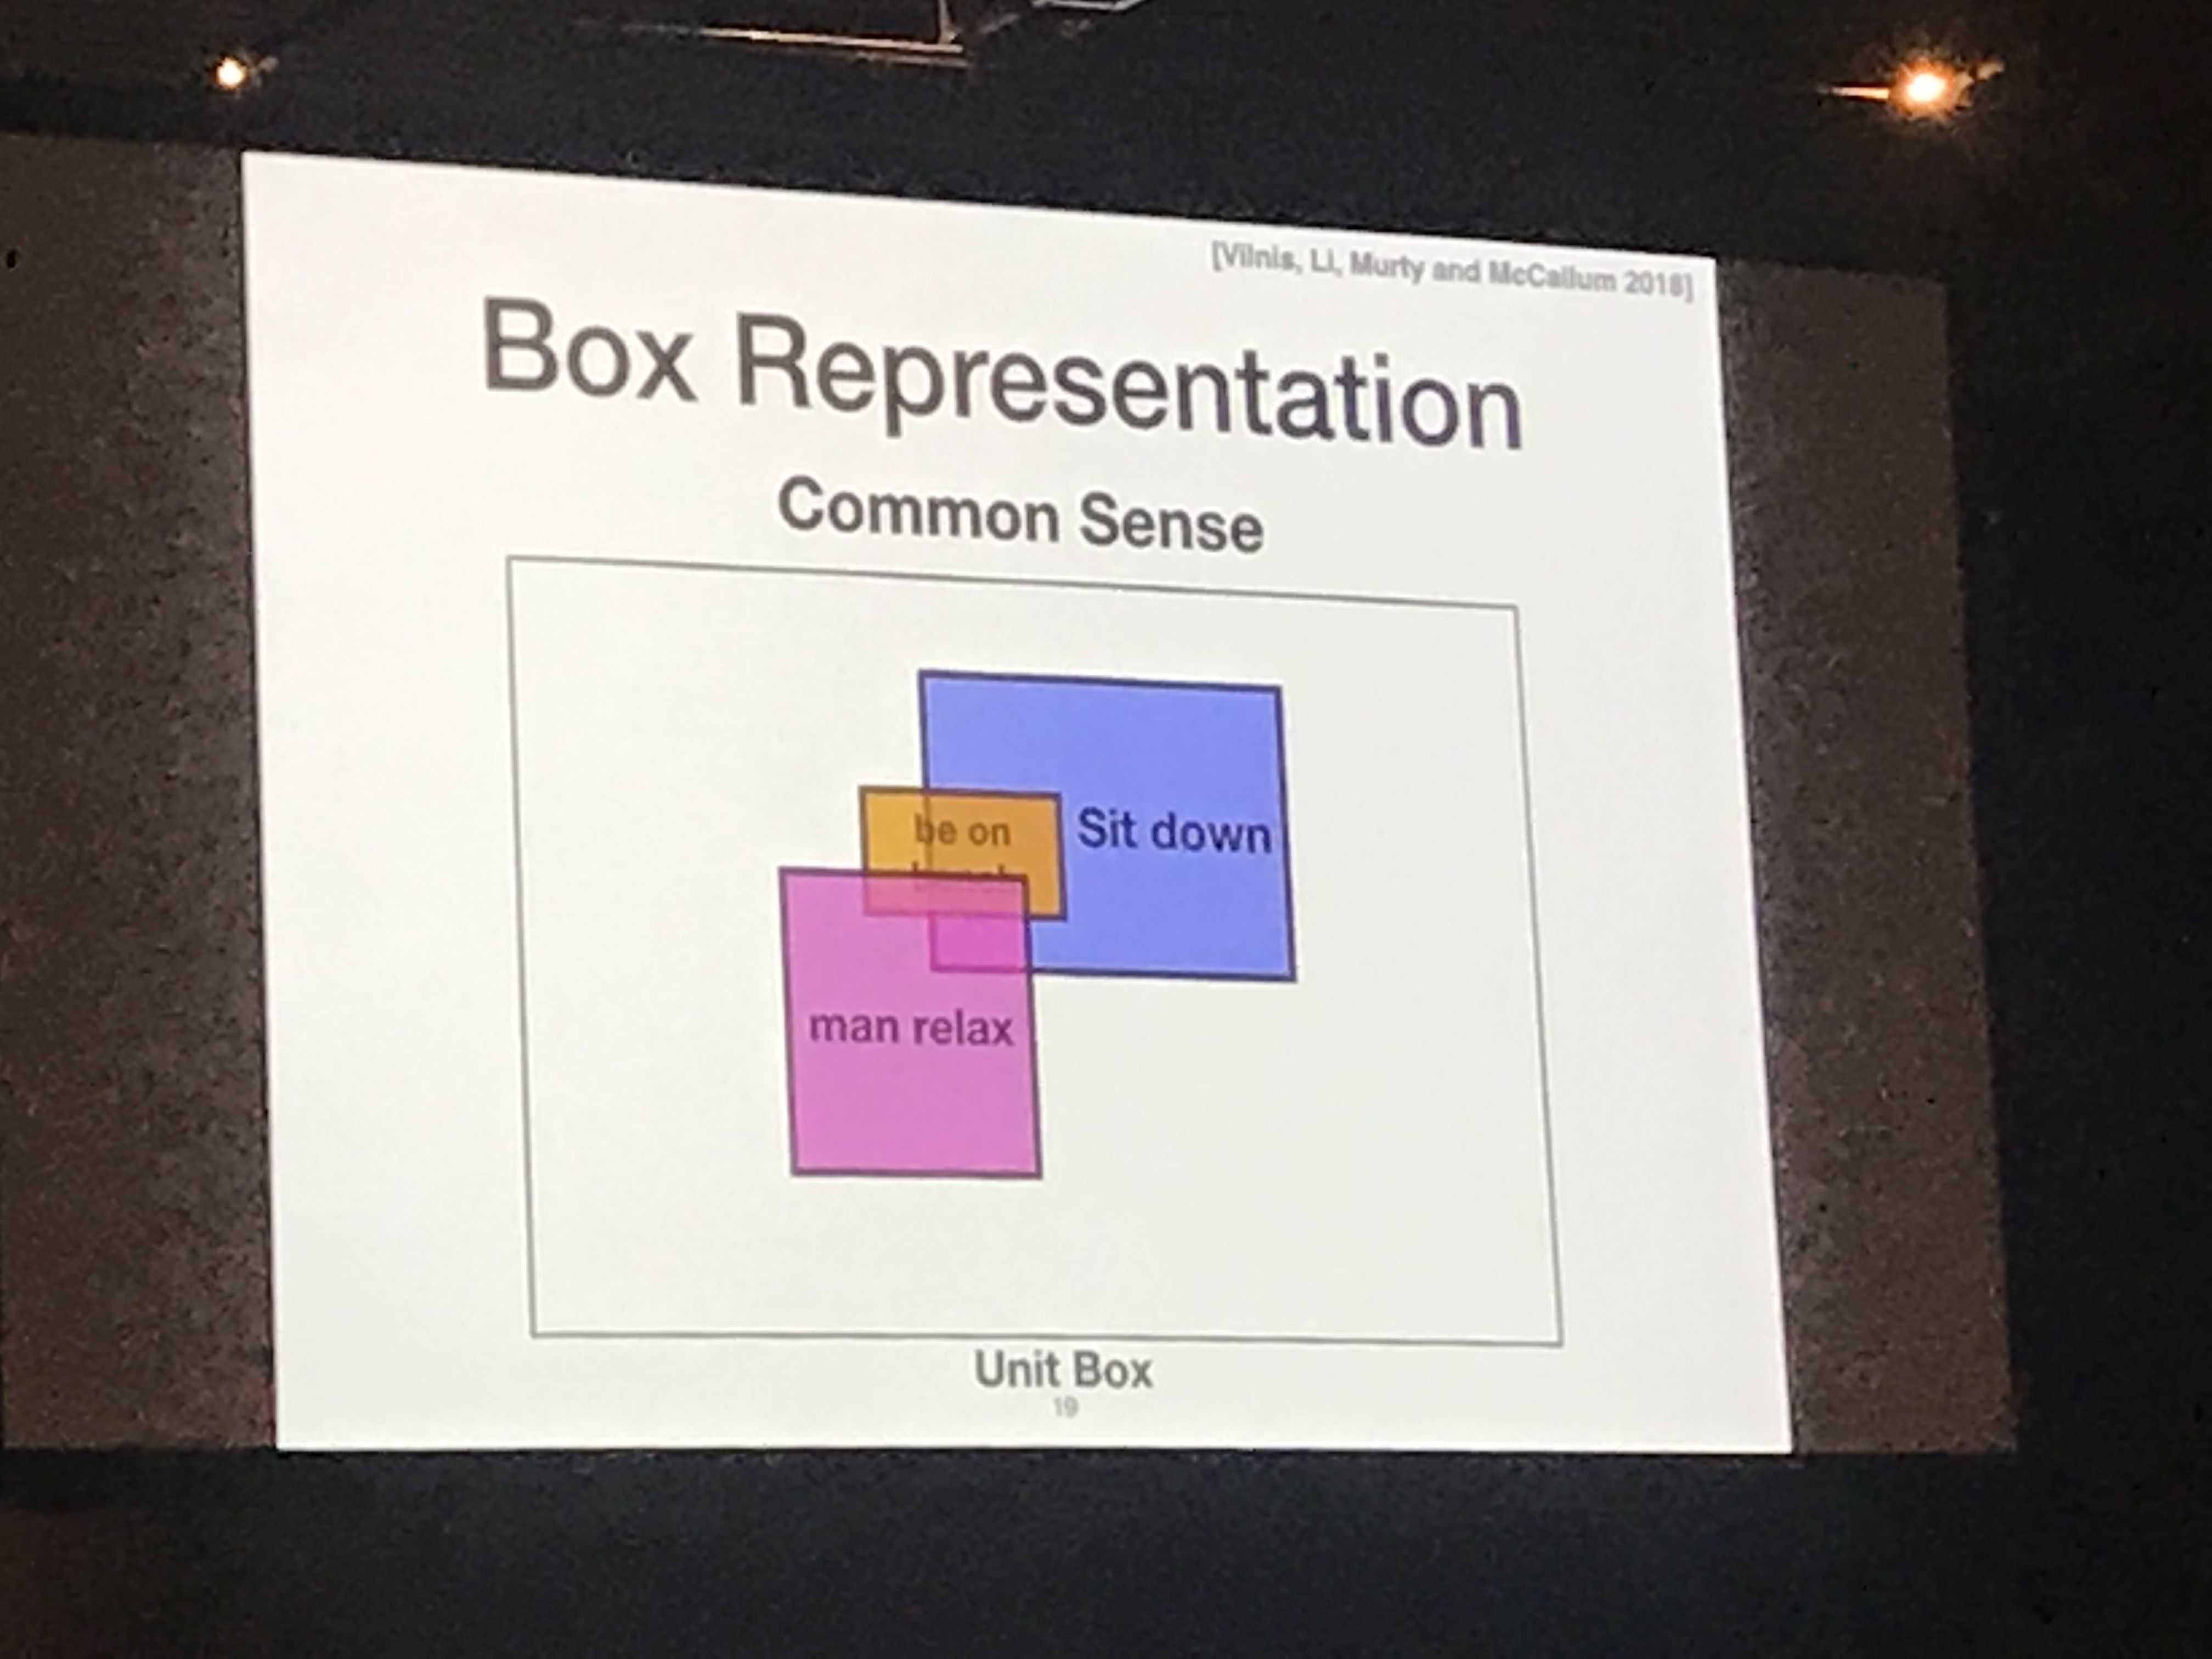
\includegraphics[width=0.4\textwidth]{images/box.JPG}
    \caption{Idea behind the new probabilistic box representation}
    \label{fig:box}
\end{figure}

Learning problem; boxes represent probability mass, try to do distribution matching over concepts. Initialize random concepts ($Pr(deer), Pr(deer \mid mammal)$. \\

{\bf Experiments:} 1) Matrix factorization in MovieLens, 2) Classification on Imbalanced Wordnet

\begin{enumerate}
    \item MovieLens Marketbase; Movie $\times$ Movie matrix: $p(lion king \mid aladdin) = 0.73)$, 286 million pairs.
    
    $\ra$ Regression task: train/dev/test, yields a matrix factorization problem (determine which movies people will like). \\
    
    $\ra$ Forrest Gump ends up being a large box, indicating that everyone likes it!
    
    \item Imbalanced WordNet: show the models learning ability for sparse, disjoint data.
    
    $\ra$ Binary classification task: achieve SOTA, even with sparse/disjoint data.
\end{enumerate}

\subsubsection{Best Paper Award Talk: Yiqang Shen on Ordered Neurons~\cite{shen2019ordered}}

{\bf Assumption:} Language has a latent tre-like structure \\

$\ra$ This work: focus on {\it constituency tree}. \\

Q: Why? \\

A1: Hierarchical representations with increasing levels of abstraction can be captured by these trees! \\

A2: Compoisitional effects of language, and long term dependency problem can be handled by these trees. \\

{\bf Main Question:} Can we provide a new inductive bias based on this tree structure to achieve a higher down stream task performance? \\

Two types of models for answering this in the past:
\begin{enumerate}
    \item Recurrent models (SPINN, RL-SPINN, RNN)
    \item Recursive models (RvNN, ST-Gumbel, DIORA)
\end{enumerate}

$\ra$ For most prior works: tree-structure given by external parser, or try to make hard decisions about how to design it. \\

{\bf This Work:} Integrate a tree structure directly into an RNN. \\

$\ra$ Tree-structure is defined by: when a larger constituent ends, all nested smaller consistuent also ends. \\

{\bf Effect:} This yields an inductive bias of ``ordered neurons", when a high ranking neuron is erased, all lower rankings neurons should also be erased. \\

To model this structure, introduce a new forget gate called the $cumax$:
\begin{equation}
    cumax(x) = cumsum(softmax(x)).
\end{equation}
Master gates for RNN:
\begin{itemize}
    \item Master forget gate:
    $\tilde{f}_t = cumax(W_f x_t + \ldots)$
    \item Master input gate:
    $\tilde{i_t} = 1 - cumax(W_f x_t + \ldots)$
\end{itemize}

{\bf Experiments:}
\begin{enumerate}
    \item Language Modeling: PTB dataset to do next-word prediction. Achieve near state of the art.
    
    \item Unsupervised Constituency Parsing: Penn TreeBank data set on language modeling task.
    
    \item Targeted Syntactic Evaluation: Marvin and Linzen dataset on a language modeling task (given a pair of similar sentences, one ungrammatical, one grammatical, see how the model performs). ON-LSTM is able to pick up on the long-term dependencies.
\end{enumerate}

Summary:
\begin{itemize}
    \item Proposed new Ordered Neuron inductive bias:
    \begin{itemize}
        \item High ranking neurons sotre long term info
        \item Low ranking neurons store short term info
    \end{itemize}
    \item New activation: $cumax()$ and ON-LSTM
    \item Inducted structure aligns with human annotated structure
    \item Stronger performance on a lot of experiments.
\end{itemize}

\dnote{And that's a wrap! Just a poster session left and then I'm off to the airport.}





% --- Bibliography ---
\newpage
\bibliographystyle{plainnat}
\bibliography{iclr}

\end{document}